\documentclass[12pt]{article}
\usepackage[a4paper,margin=1in]{geometry}
\usepackage{graphicx}
\usepackage{enumitem}
\usepackage{xurl}
\usepackage{hyperref}
\usepackage{xcolor}
\usepackage{listings}

\setlength{\parskip}{0.6em}
\setlength{\parindent}{0pt}

\title{Image Gallery Platform -- Implementation Report}
\author{}
\date{\today}

\begin{document}
\sloppy
\begin{titlepage}
\centering
\vspace*{1cm}

\includegraphics[width=0.95\textwidth]{media/cf.png}\\[1.5cm]
{\LARGE \bfseries Image Gallery Platform -- Implementation Report\\[0.5cm]}
{\large \today}
\end{titlepage}

\section{Summary}
This project implements a globally distributed image gallery API using Cloudflare’s developer platform services. It securely stores images, delivers them through the Cloudflare edge network, and automatically enriches them with descriptive \textbf{Alt-Text} generated by AI vision models, in case it was not initially provided.

The solution is currently hosted in \href{https://image-gallery.goncalo2k.pt}{image-gallery.goncalo2k.pt} and its Github repo is under \href{https://github.com/goncalo2k/image-gallery}{goncalo2k/image-gallery}.

The solution is designed to improve \textbf{performance, accessibility, and operational efficiency} while minimizing infrastructure costs and complexity. Images are stored in \textbf{Cloudflare R2}, delivered through \textbf{Cloudflare Workers}, and enriched using \textbf{Workers AI Image-to-Text models}. Generated descriptions and metadata are persisted in a \textbf{D1 database}, ensuring that each image is processed only once and avoiding unnecessary costs when processing images. The requests for specific images are cached and invalidated uppon image deletion using \textbf{Cloudflare's Cache API}, which allows frequently requested images to be served directly from edge locations around the world, therefore optimizing performance and reducing compute usage.

Additionally, the system includes administrative and operational capabilities such as:
\begin{itemize}[leftmargin=*]
  \item An \textbf{audit endpoint} for inspecting processed images and their metadata
  \item \textbf{Dynamic image ingestion} from external URLs
  \item \textbf{Image ingestion} from local files
  \item Delete images previously uploaded
  \item List all images currenty available
  \item Secure service-to-service communication between storage, compute, and database layers thanks to Worker Bindings
\end{itemize}

\pagebreak


\section{Solution Requirements}
The initial requirements presented for this product were the following:

\subsection{Business Requirements}
\begin{itemize}[leftmargin=*]
  \item The platform must provide a scalable and globally accessible image delivery service capable of serving images with descriptive metadata to improve accessibility.
  \item The system must automatically generate and manage descriptive alt-text for images to enhance accessibility compliance and improve user experience.
  \item The platform must minimize operational costs by leveraging edge caching and efficient AI inference usage.
  \item The system must maintain a persistent and auditable record of processed images and their associated metadata.
  \item The platform must support automated ingestion of new image assets to streamline content management workflows.
  \item The system must enforce secure storage and controlled access to image assets and administrative interfaces.
\end{itemize}

\subsection{Functional Requirements}
\begin{itemize}[leftmargin=*]
  \item Image Storage: The system must initialize a private Cloudflare R2 bucket and it must be populated with a small set of sample images for testing.
  \item Edge Image Delivery: A Cloudflare Worker must serve images directly to web browsers. Each image response must include a descriptive alt-text string in a custom HTTP header.
  \item Alt-Text Generation: The system must generate image descriptions using Workers AI vision models when alt-text is not available. This should be done while respecting Workers AI daily neuron limits. The system must avoid re-running inference for images that have already been processed.
  \item Persistent Metadata Storage: A Cloudflare D1 database must store generated alt-text descriptions and associated image metadata. The system must query the database to determine whether an image has already been processed.
  \item Caching and Performance: The system must leverage Cloudflare's Cache API for performance and compute optimization. The architecture must also leverage non-blocking background operations so image delivery is not delayed by database or AI processing.
  \item Administrative Endpoint: A secure \texttt{/audit} endpoint must return a JSON list of processed images and their stored metadata from D1.
  \item Dynamic Image Ingestion: The system must allow new images to be ingested from an external URL, storing them in the R2 bucket and automatically triggering description generation and metadata storage.
\end{itemize}

\subsection{Security Requirements}
\begin{itemize}[leftmargin=*]
  \item Secure Storage: The R2 bucket must remain private and inaccessible directly from the public internet.
  \item Endpoint Protection: Administrative endpoints (e.g., \texttt{/audit}) must require secure access controls.
  \item Environment Security: Secrets (API keys, tokens, database credentials) must be stored using Cloudflare environment variables or secret management.
\end{itemize}

\section{Real Use Cases}
This API was designed to be used by other services in a variety of ways. Possible use cases are:
\begin{enumerate}[leftmargin=*]
  \item \textbf{Editorial portfolio backend} – The Worker powers a personal portfolio that cycles through stored images. A back-office or CMS jobs call \texttt{/images/external} with curated URLs or actual files, the Worker stores binaries in R2, generates Workers AI alt text, and exposes metadata via \texttt{/images} and \texttt{/images/:id}. The BFF API that powers the Frontend consumes the \texttt{/images} and \texttt{/images/:id} endpoints to get the images and serves them to the Frontend, for them to be dynamically displayed in a caroussel, while leveraging the caching at the Edge level.
  \item \textbf{Internal design library} – A design team mirrors approved brand assets by uploading local files through \texttt{/images}. D1 metadata acts as the source of truth for descriptions, while \texttt{GET /images/audit} feeds a Notion dashboard that tracks total assets and most recent updates, from which the users can select images and get redirected to the \texttt{/images/:id} endpoint, that serves the selected image alongisde with its alt-text.
\end{enumerate}

\section{Customer Experience}
The focus of this API is to fulfill the systems' requirements without compromising the developer experience. While developing this product, there was a big emphasis on producing a smooth experience for systems and developers utilizing this API.
\begin{itemize}[leftmargin=*]
  \item \textbf{Fast delivery} – Images stream from Cloudflare’s edge with cache hits served immediately and cache misses still benefitting from R2’s proximity to Workers. Predictable latency keeps portfolio visitors and internal stakeholders engaged.
  \item \textbf{Accessible by default} – Every response exposes descriptive text through \texttt{ALT\_HEADER\_NAME}, so consuming apps can provide meaningful alt text without a separate metadata fetch.
  \item \textbf{Self-service operations} – The REST surface is minimal (\texttt{/images}, \texttt{/images/:id}, \texttt{/images/audit}), and the OpenAPI schema + Swagger UI give non-engineers an explorable contract. Scripts handle common chores (bulk upload/clear), reducing toil for content teams.
  \item \textbf{Secure touchpoints} – Cloudflare Access service tokens, CORS allow-lists, and timing-safe credential checks ensure that only trusted systems can mutate the gallery, while public endpoints (\texttt{/health}, \texttt{/docs}, \texttt{/openapi.json}) remain open for observability.
\end{itemize}

\section*{Setup Instructions}
\subsection{Local development:}

\subsubsection{Prerequisites:}
\begin{enumerate}[leftmargin=*]
  \item Install NPM or PNPM;
\end{enumerate}

\subsection{Local Setup}
\begin{enumerate}[leftmargin=*]
  \item Clone the \href{https://github.com/goncalo2k/image-gallery}{github repo}
  \item Install dependencies using \texttt{npm i} or \texttt{pnpm i}
  \item Update \texttt{wrangler.jsonc} to contain the desired \texttt{routes} and \texttt{custom\_domains}, the bindings for \texttt{d1\_databases} and \texttt{r2\_buckets} as well as the Woker's \texttt{name}. Note that you can use the database and bucket bindings with local or remote versions.
  \item Copy \texttt{.dev.vars.example} and rename it to \texttt{.dev.vars}, updating the values inside.
  \item For local D1 setup, run \texttt{npm run setup-local-db} or \texttt{pnpm run setup-local-db}.
  \item (Optional) To populate the database and the blob storage, use \texttt{npm run batch-upload} or \texttt{pnpm run batch-upload}.
  \item (Optional) To purge both D1 and R2, run \texttt{npm run clear-images} or \texttt{pnpm run clear-images}.
  \item Run \texttt{npm run cf-typegen} or \texttt{pnpm run cf-typegen} to generate types.
  \item Then, just run the Worker with \texttt{npm dev} or \texttt{pnpm dev}
\end{enumerate}

Note that, on every commit, both \texttt{pnpm lint} \&\& \texttt{pnpm test} are run to ensure nothing is broken.

\section{Instructions to Use the Platform \& Testing Evidence}
Note that all endpoints work exactly the same in the deployed version and in the local version and to test locally, running the worker on your local machine and changing from \texttt{https://image-gallery.goncalo2k.pt} to \texttt{http://localhost:8787}. However, the deployed \texttt{/audit} has an extra layer of security due to the \textbf{Access Policy} previously defined and the \textbf{401 Response for Service Auth} being enabled. Also note that all the endpoints are present in the postman collection under the folder \texttt{postman} of the repo.

\subsection{Viewing Images}
Hit \texttt{GET https://image-gallery.goncalo2k.pt/images} to retrieve paginated metadata (\texttt{offset}, \texttt{limit} query params). Fetch an individual asset with \texttt{GET https://image-gallery.goncalo2k.pt/images/{id}}; successful responses include \texttt{Content-Type}, cache headers, and \texttt{ALT\_HEADER\_NAME} for instant consumption in web browsers.

\subsubsection{Testing Evidence}

\begin{figure}[h]
\centering
\begin{minipage}{0.32\textwidth}
\centering
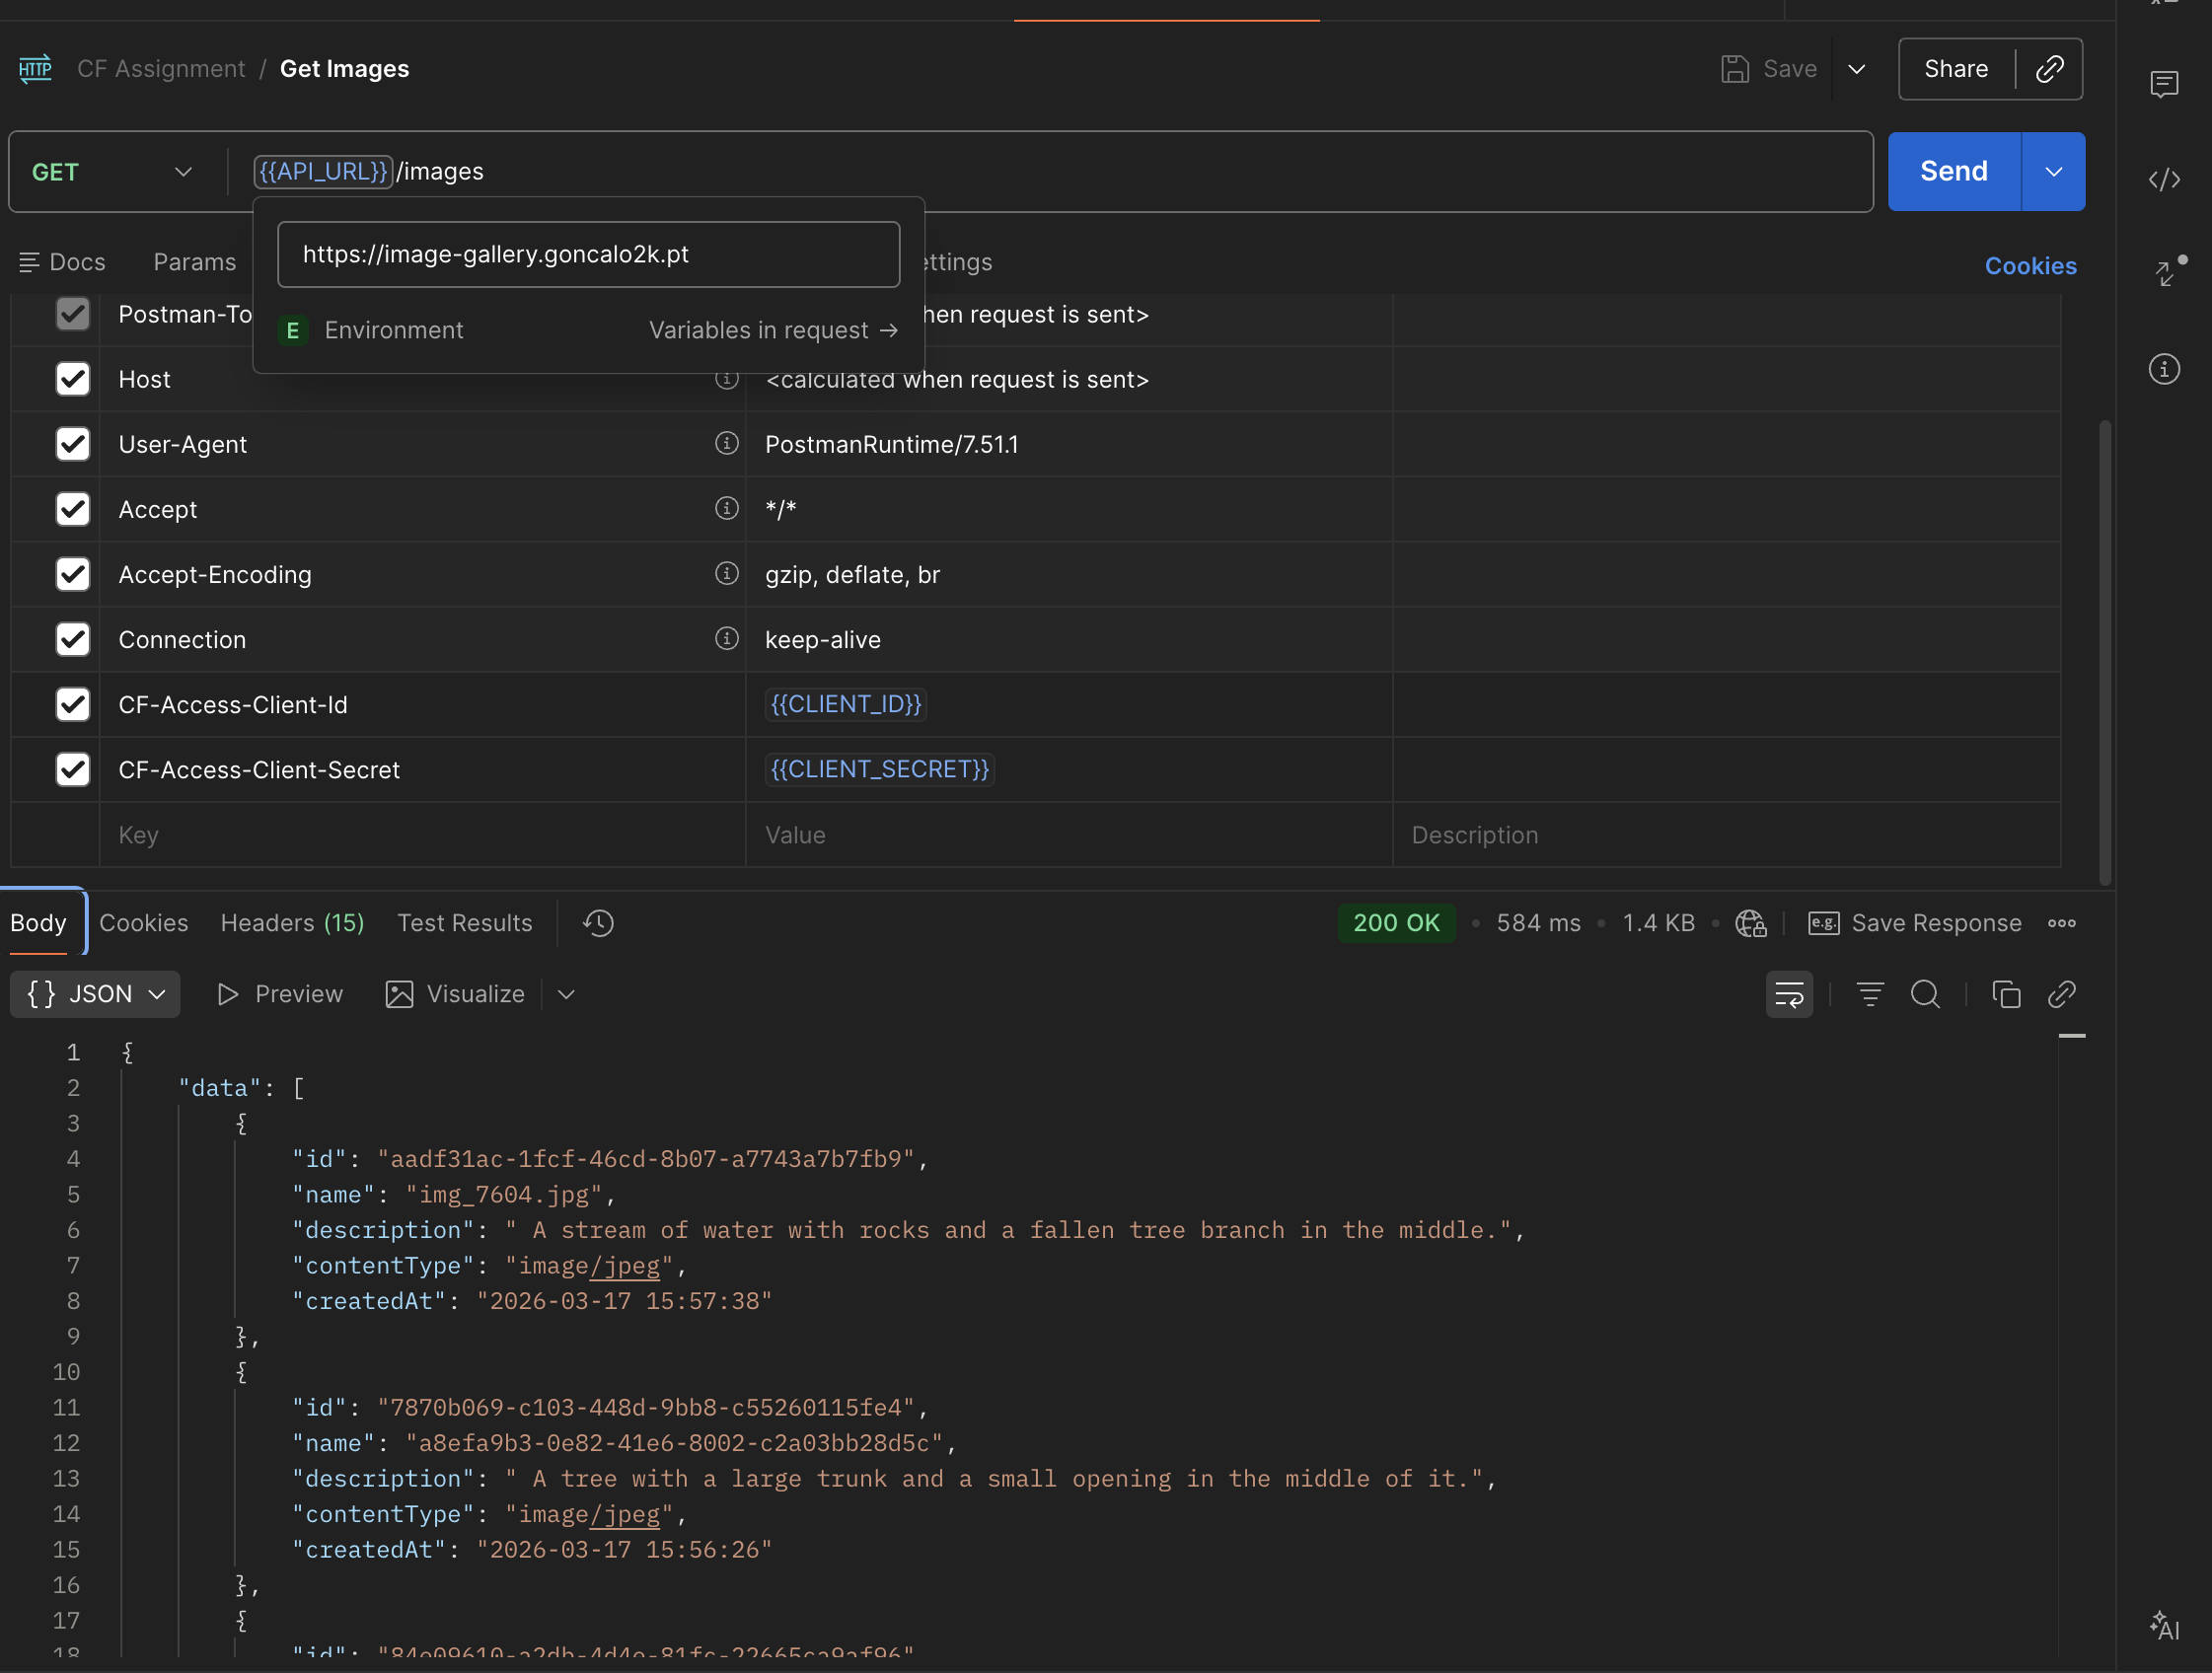
\includegraphics[width=\linewidth]{media/testing-evidence/images-success.png}
\end{minipage}
\begin{minipage}{0.32\textwidth}
\centering
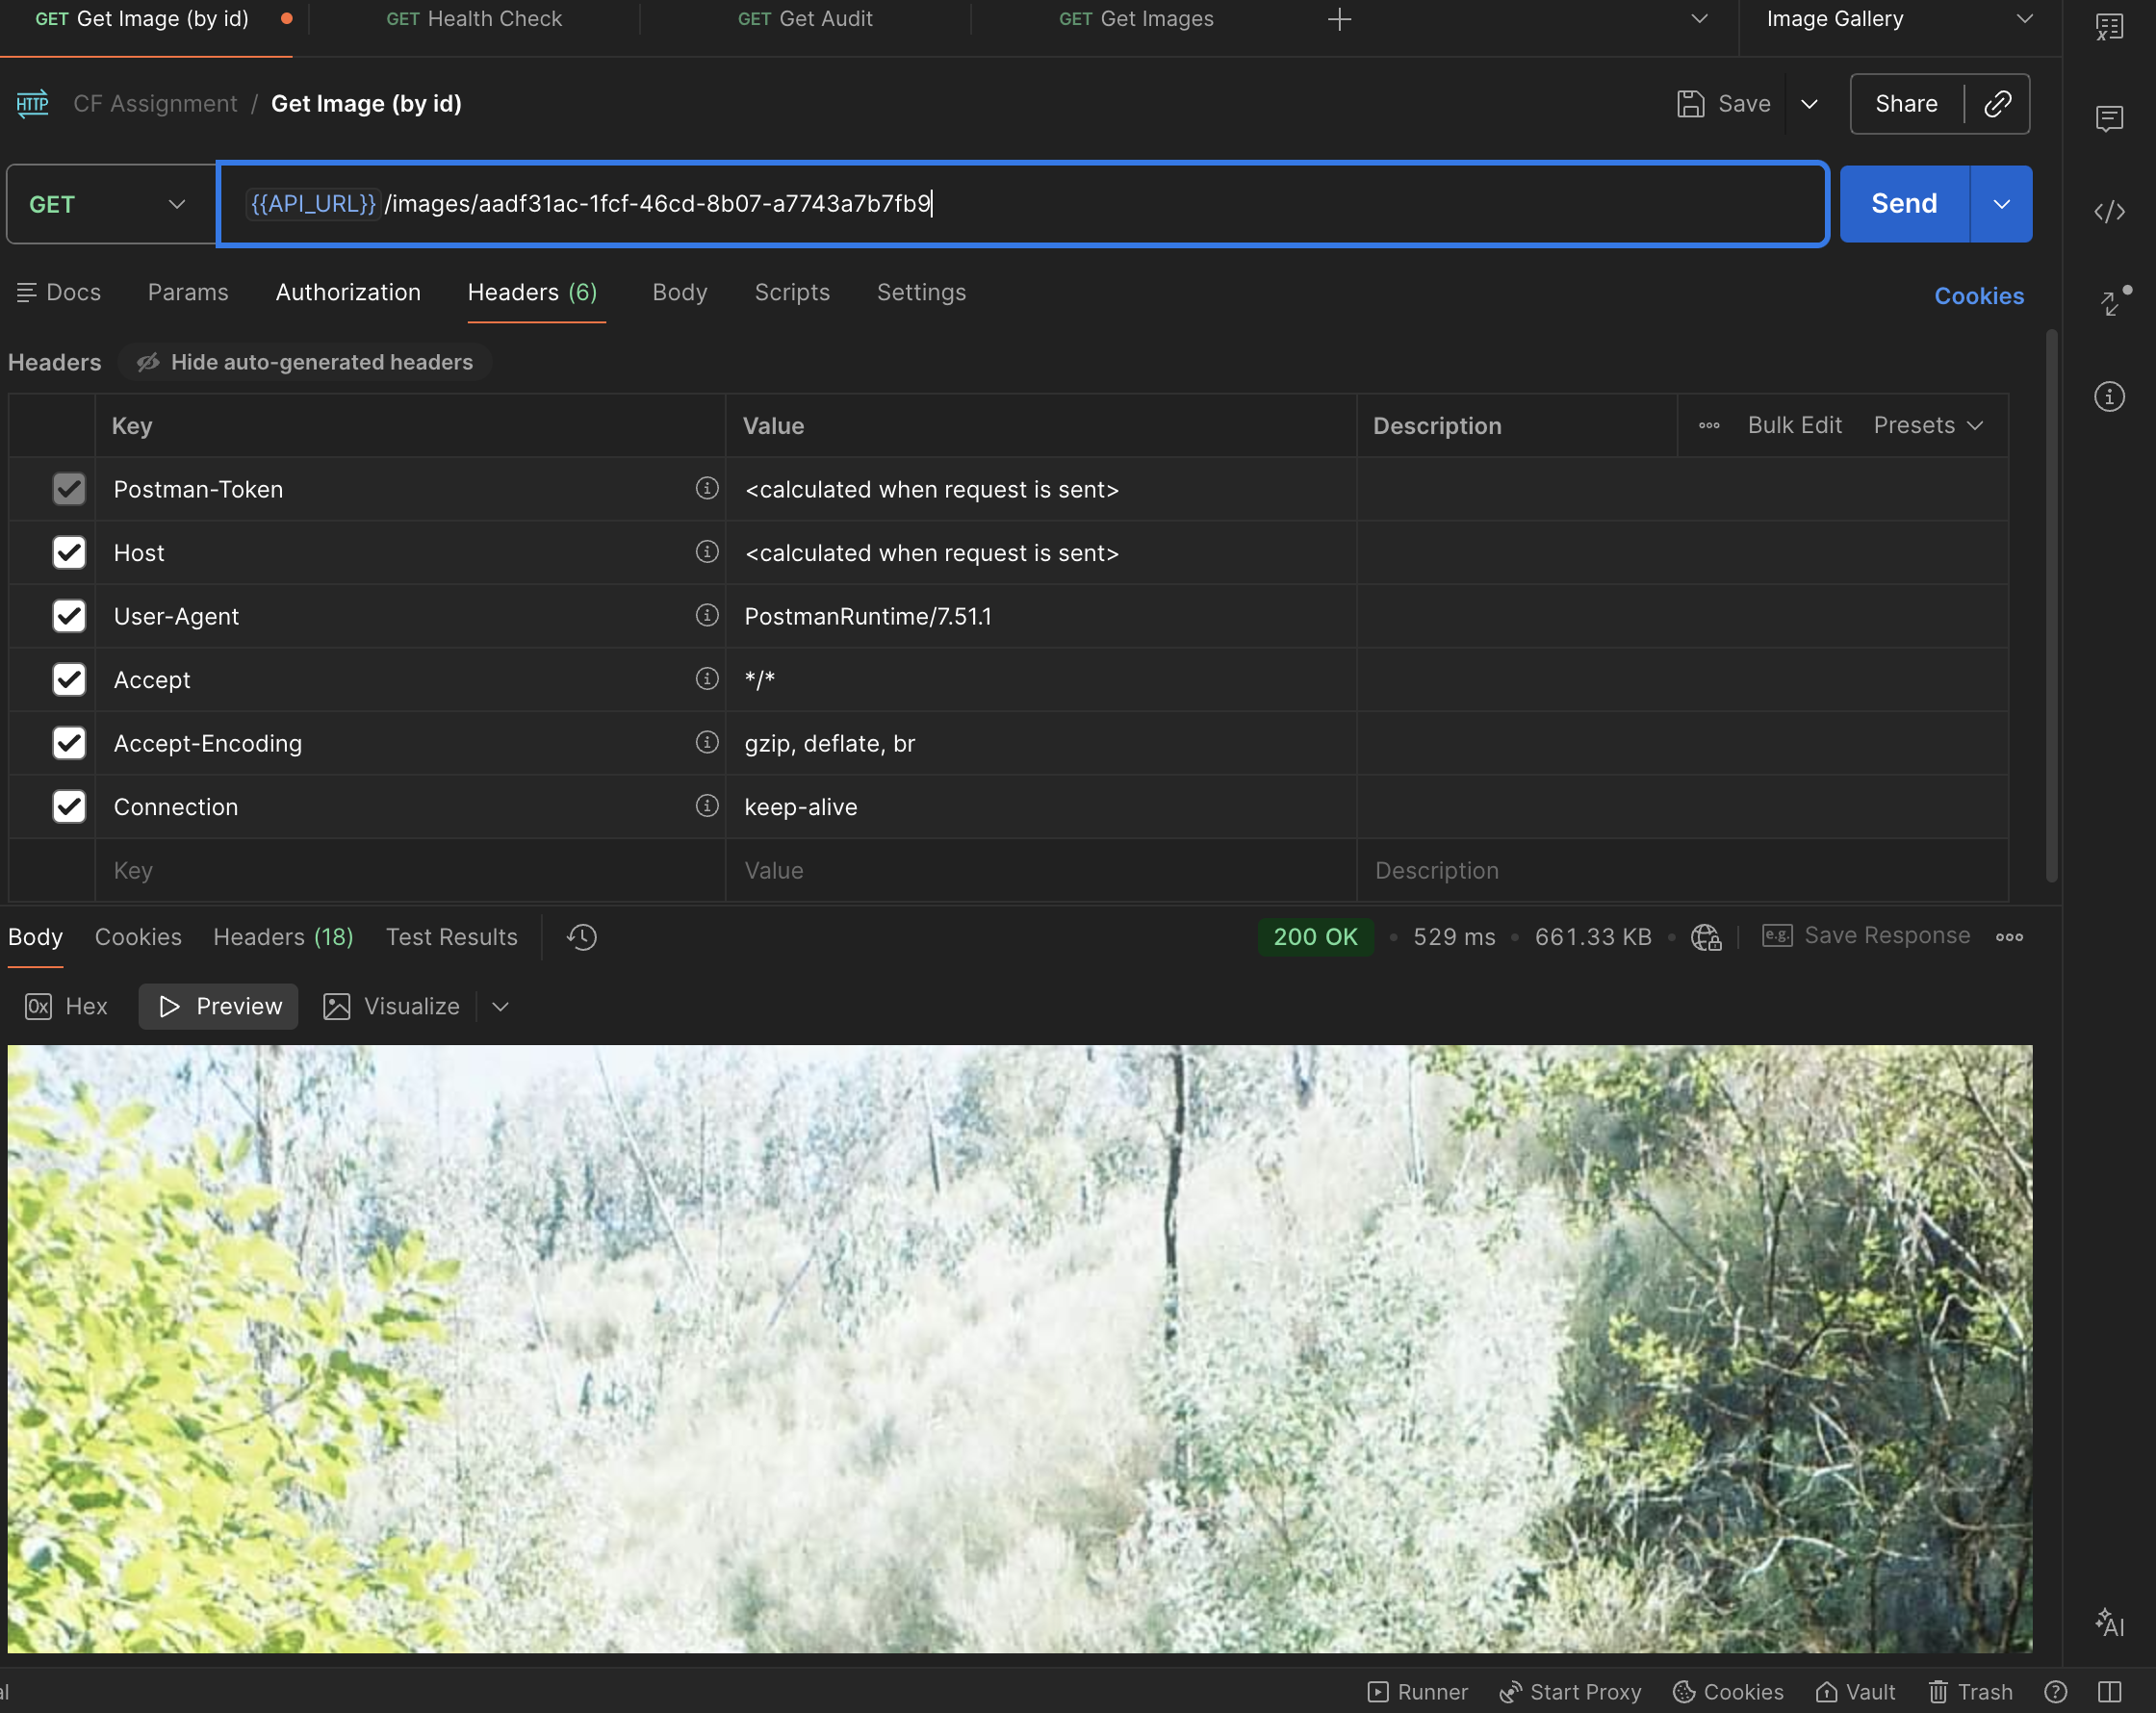
\includegraphics[width=\linewidth]{media/testing-evidence/images-id-success.png}
\end{minipage}
\begin{minipage}{0.32\textwidth}
\centering
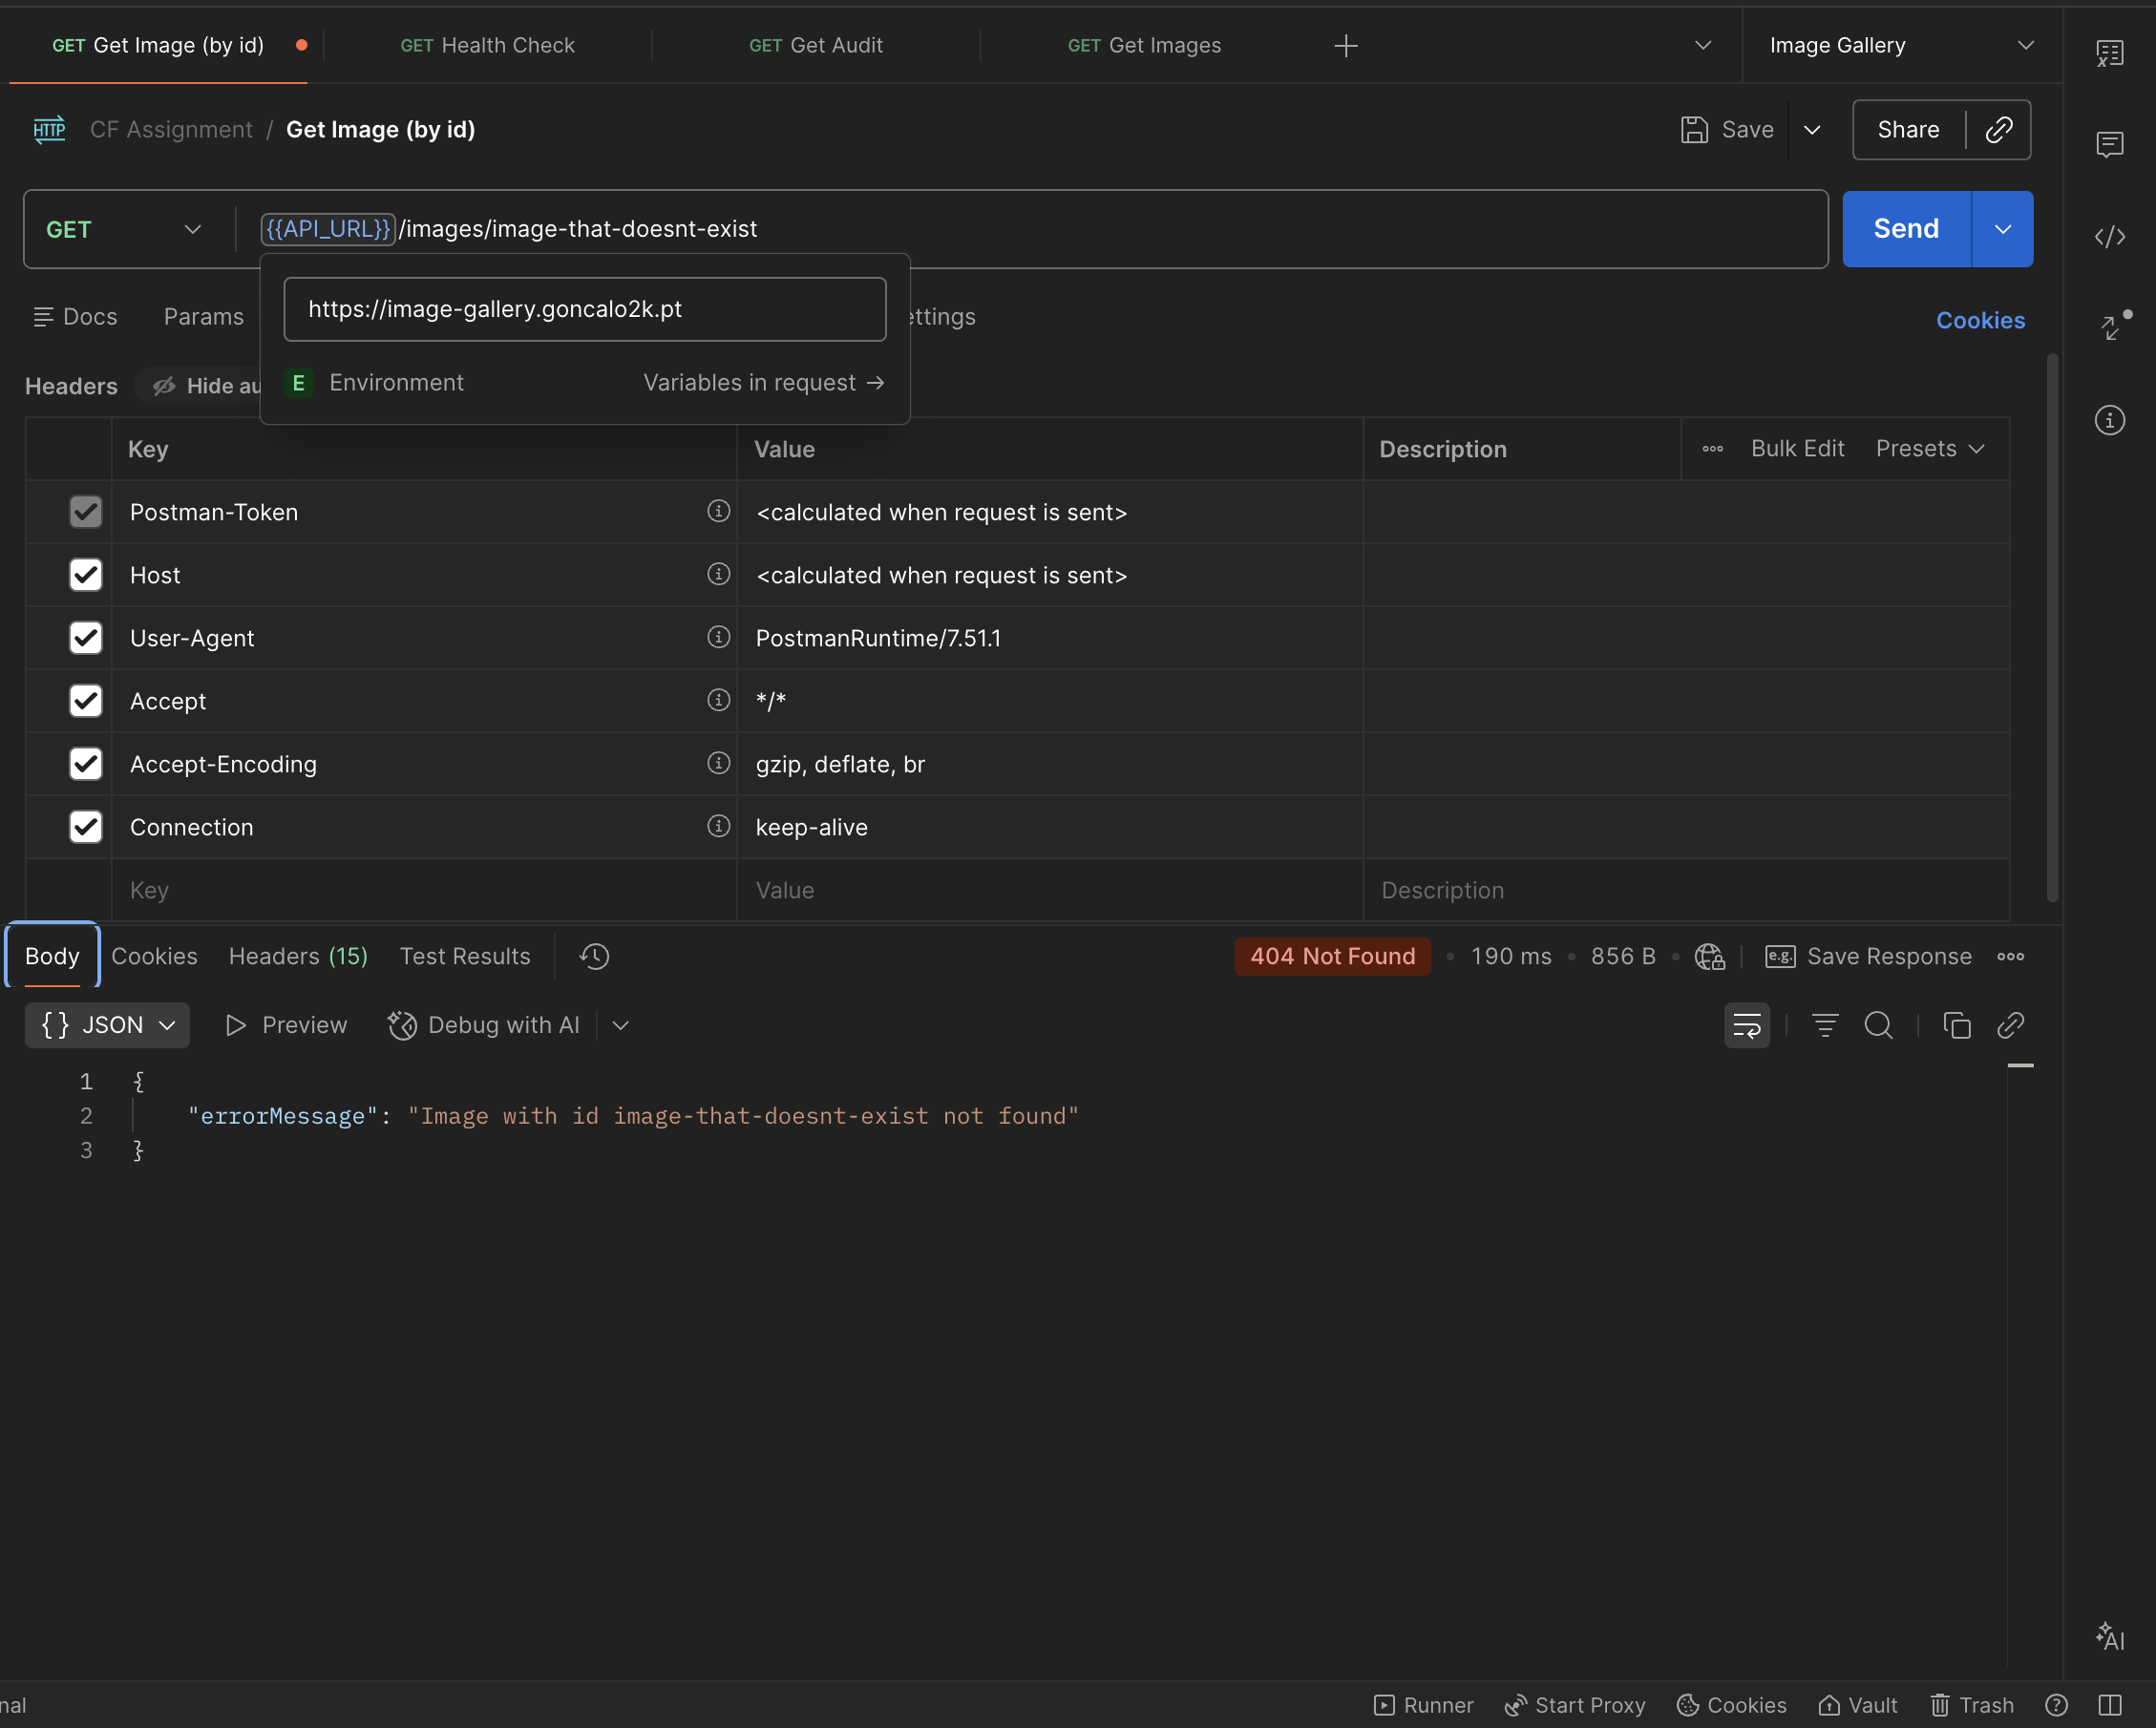
\includegraphics[width=\linewidth]{media/testing-evidence/images-id-failure.png}
\end{minipage}
\end{figure}

\subsection{Ingesting Images}
Hit \texttt{POST https://image-gallery.goncalo2k.pt/images} with fields \texttt{file}, \texttt{name?}, and \texttt{description?}. To ingest from a remote URL, POST to \texttt{/images/external} with \texttt{fileUrl}, \texttt{name?}, \texttt{description?}.

\subsubsection{Testing Evidence}

\begin{figure}[h]
\centering
\begin{minipage}{0.32\textwidth}
\centering
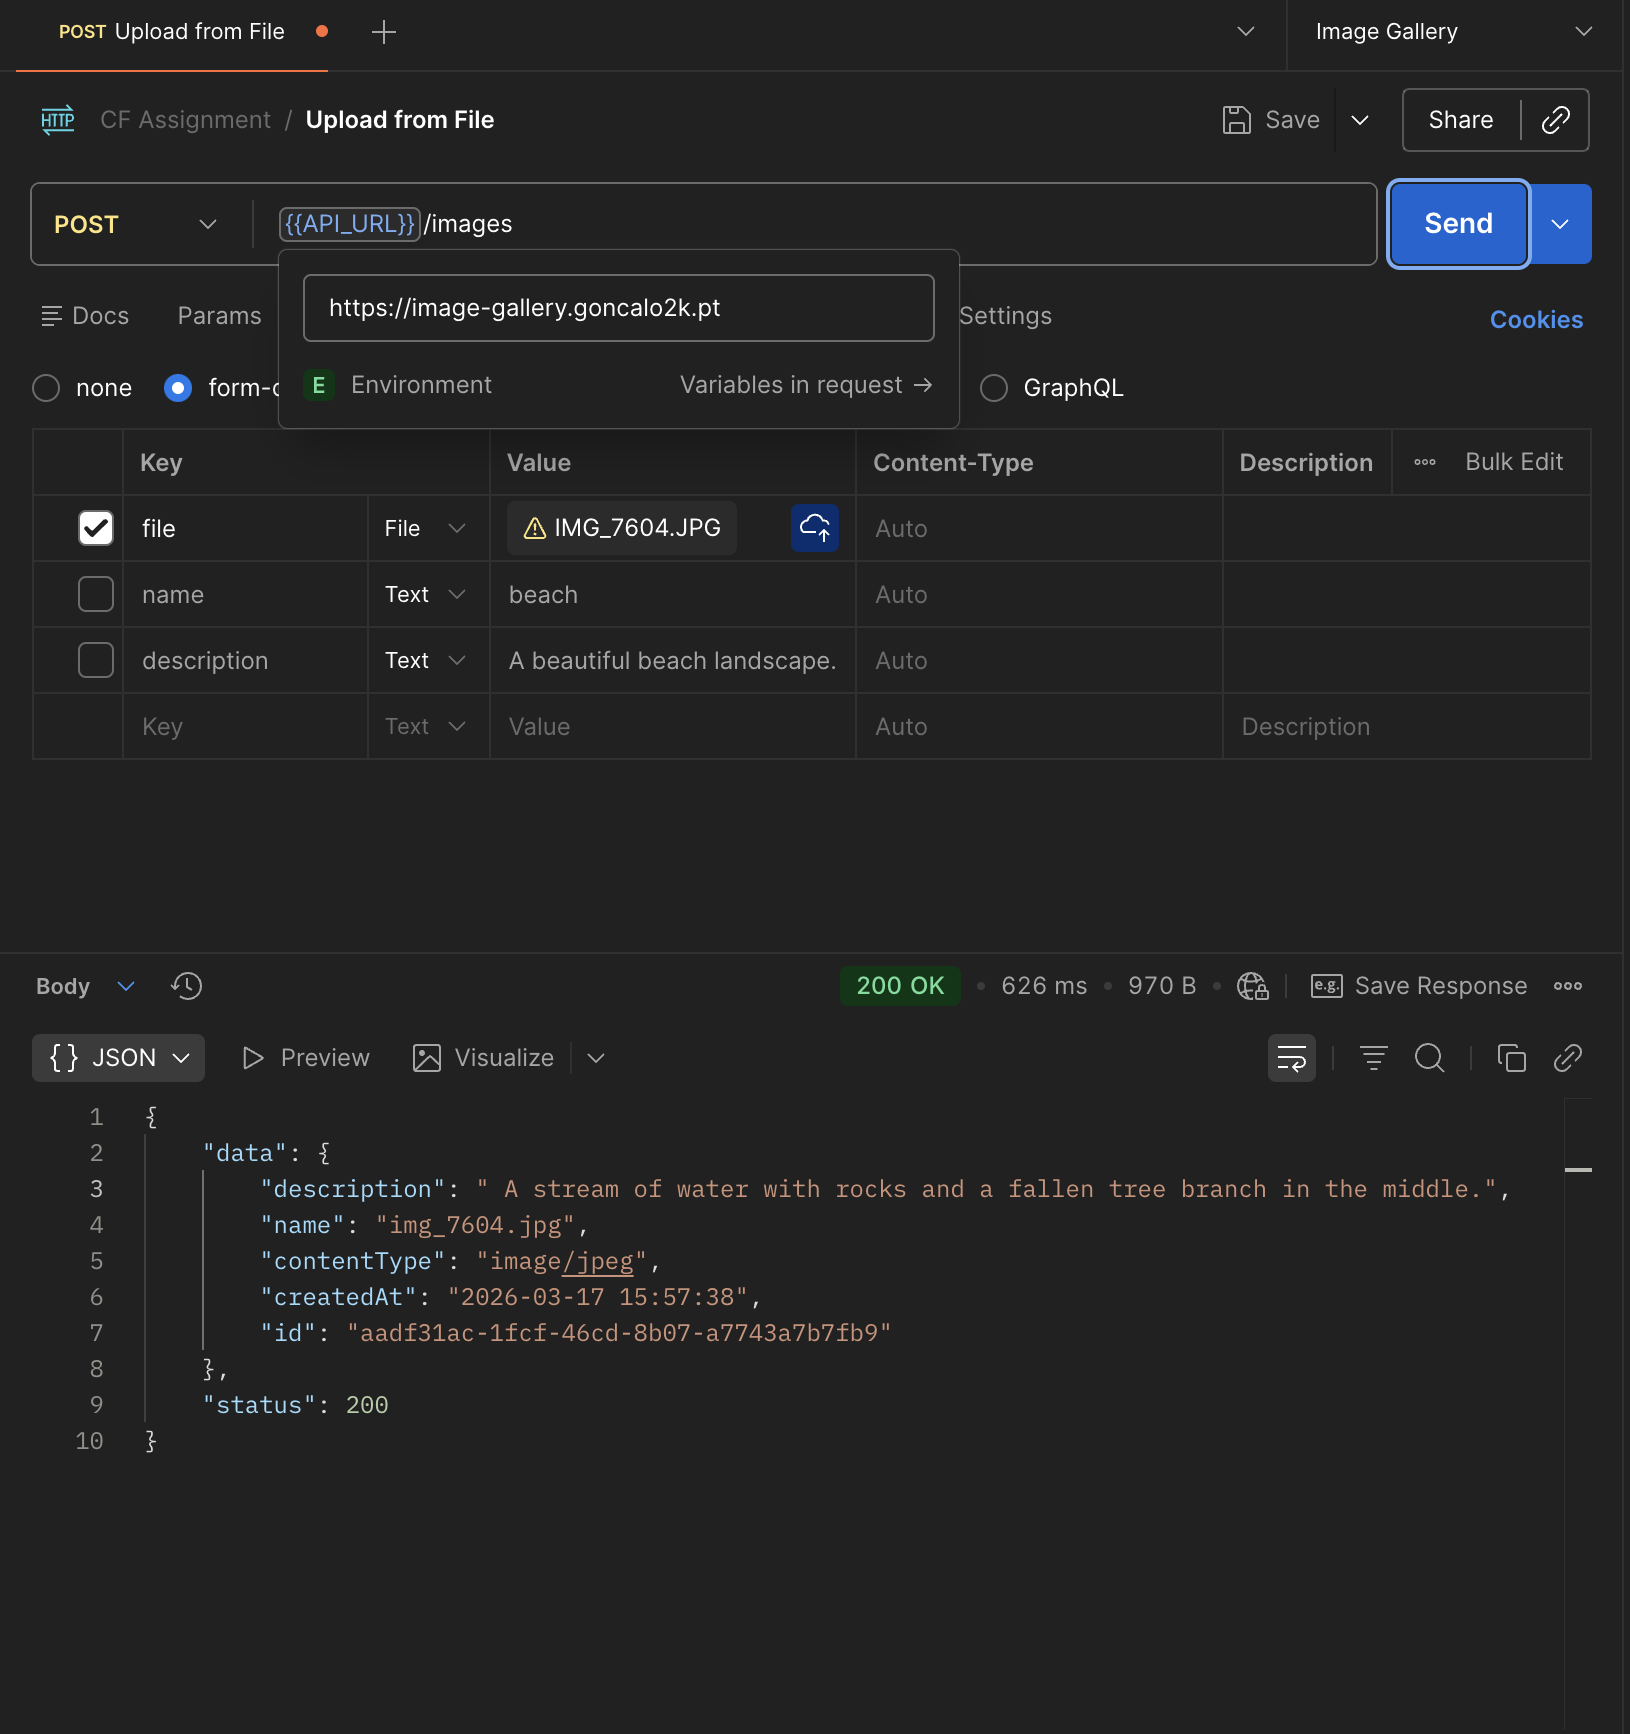
\includegraphics[width=\linewidth]{media/testing-evidence/upload-file-success-already-existent.png}
\end{minipage}
\begin{minipage}{0.32\textwidth}
\centering
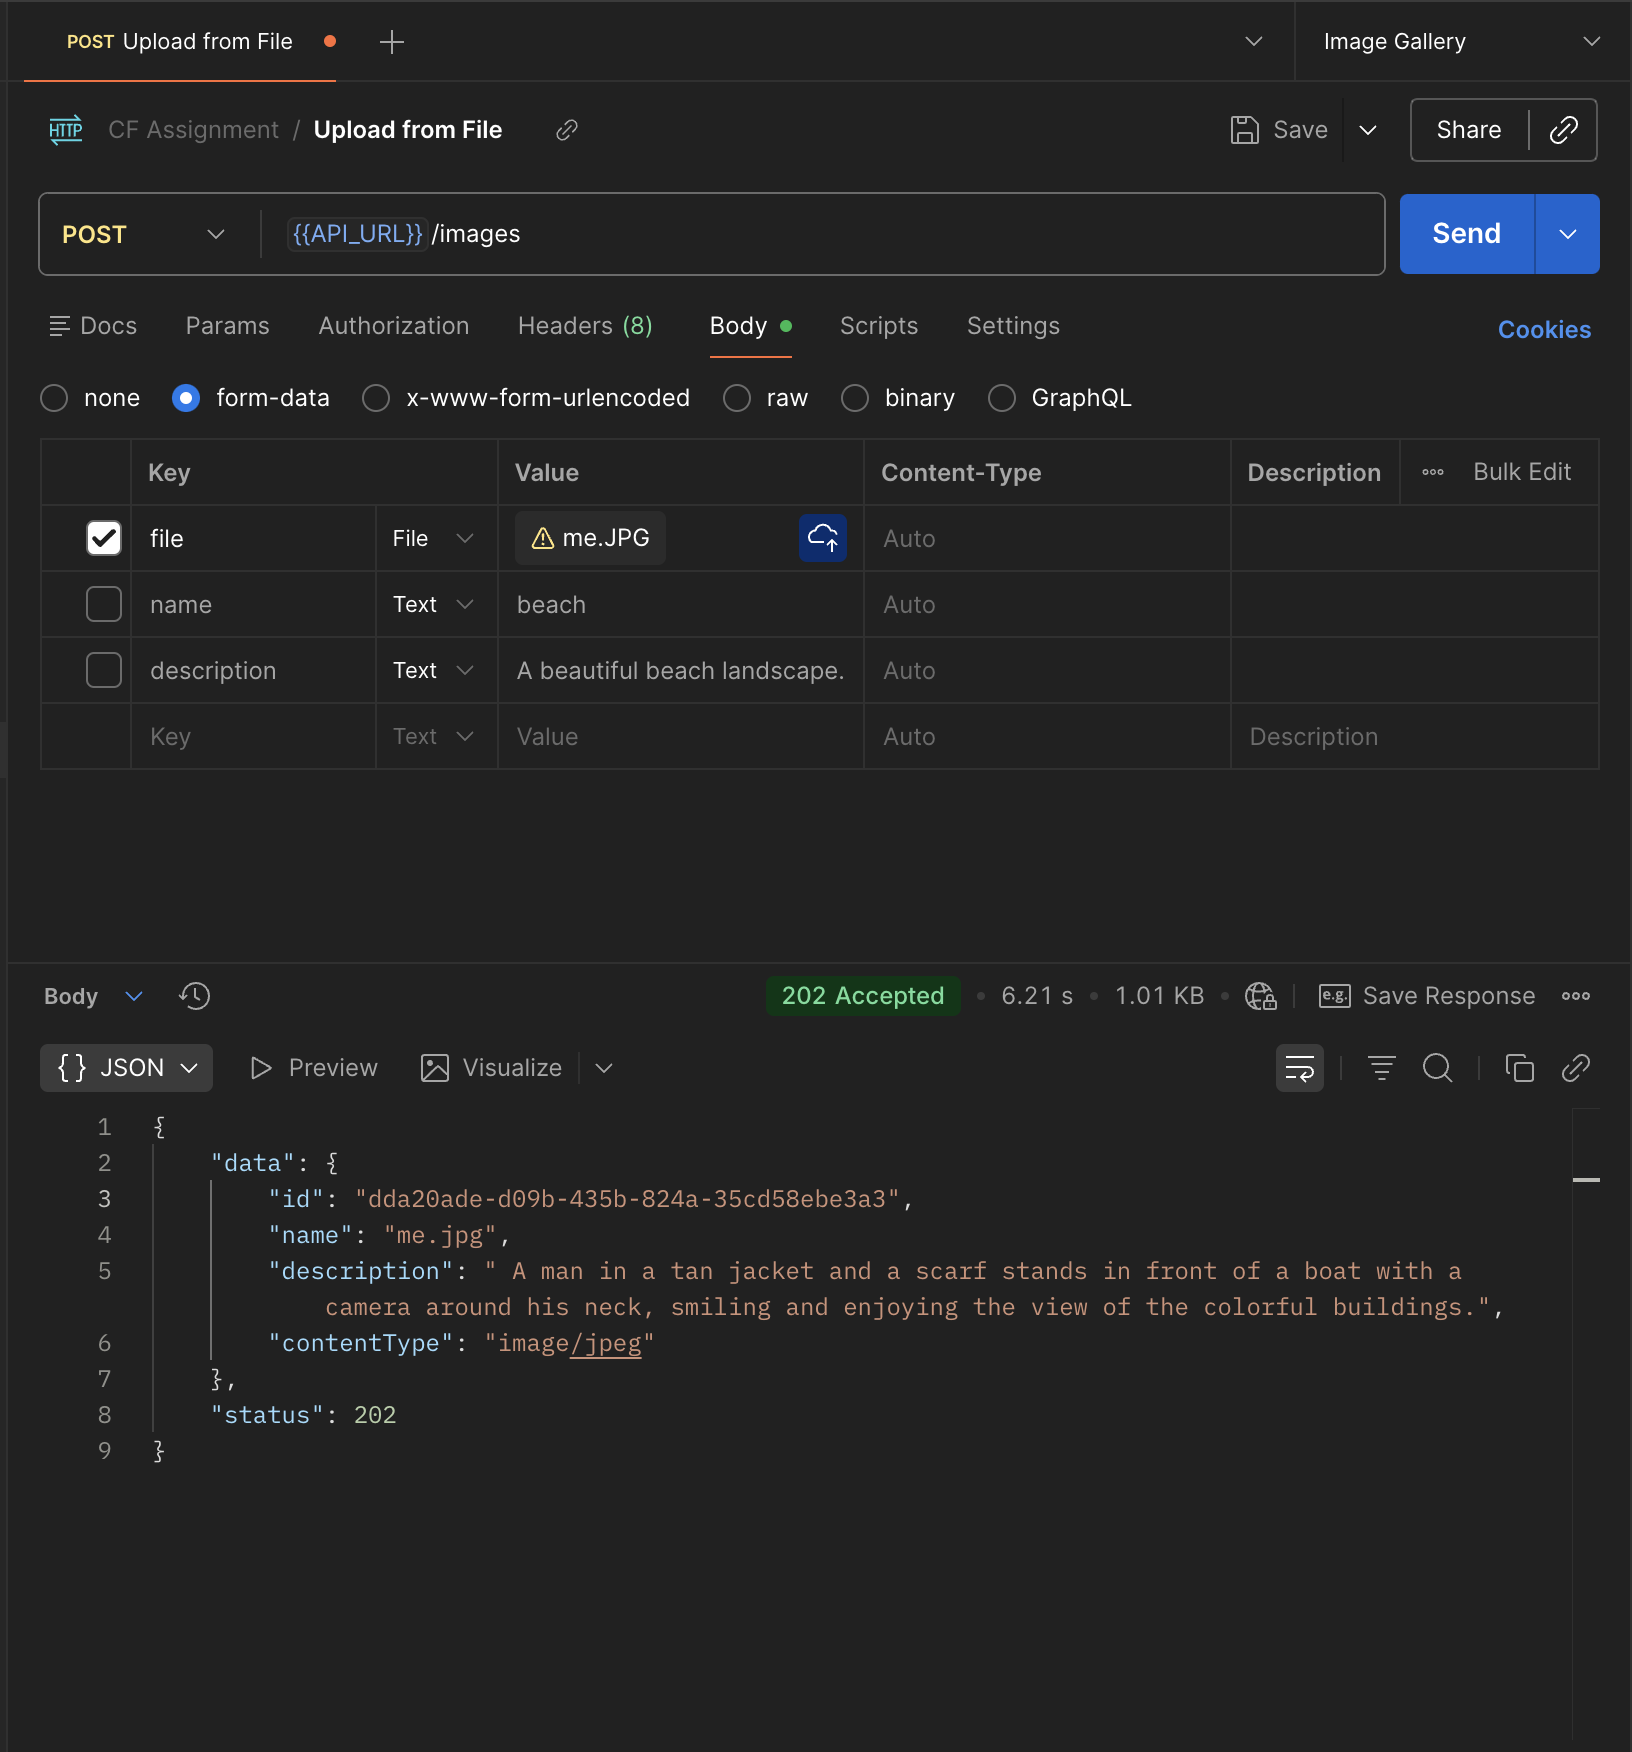
\includegraphics[width=\linewidth]{media/testing-evidence/upload-file-success-new.png}
\end{minipage}
\begin{minipage}{0.32\textwidth}
\centering
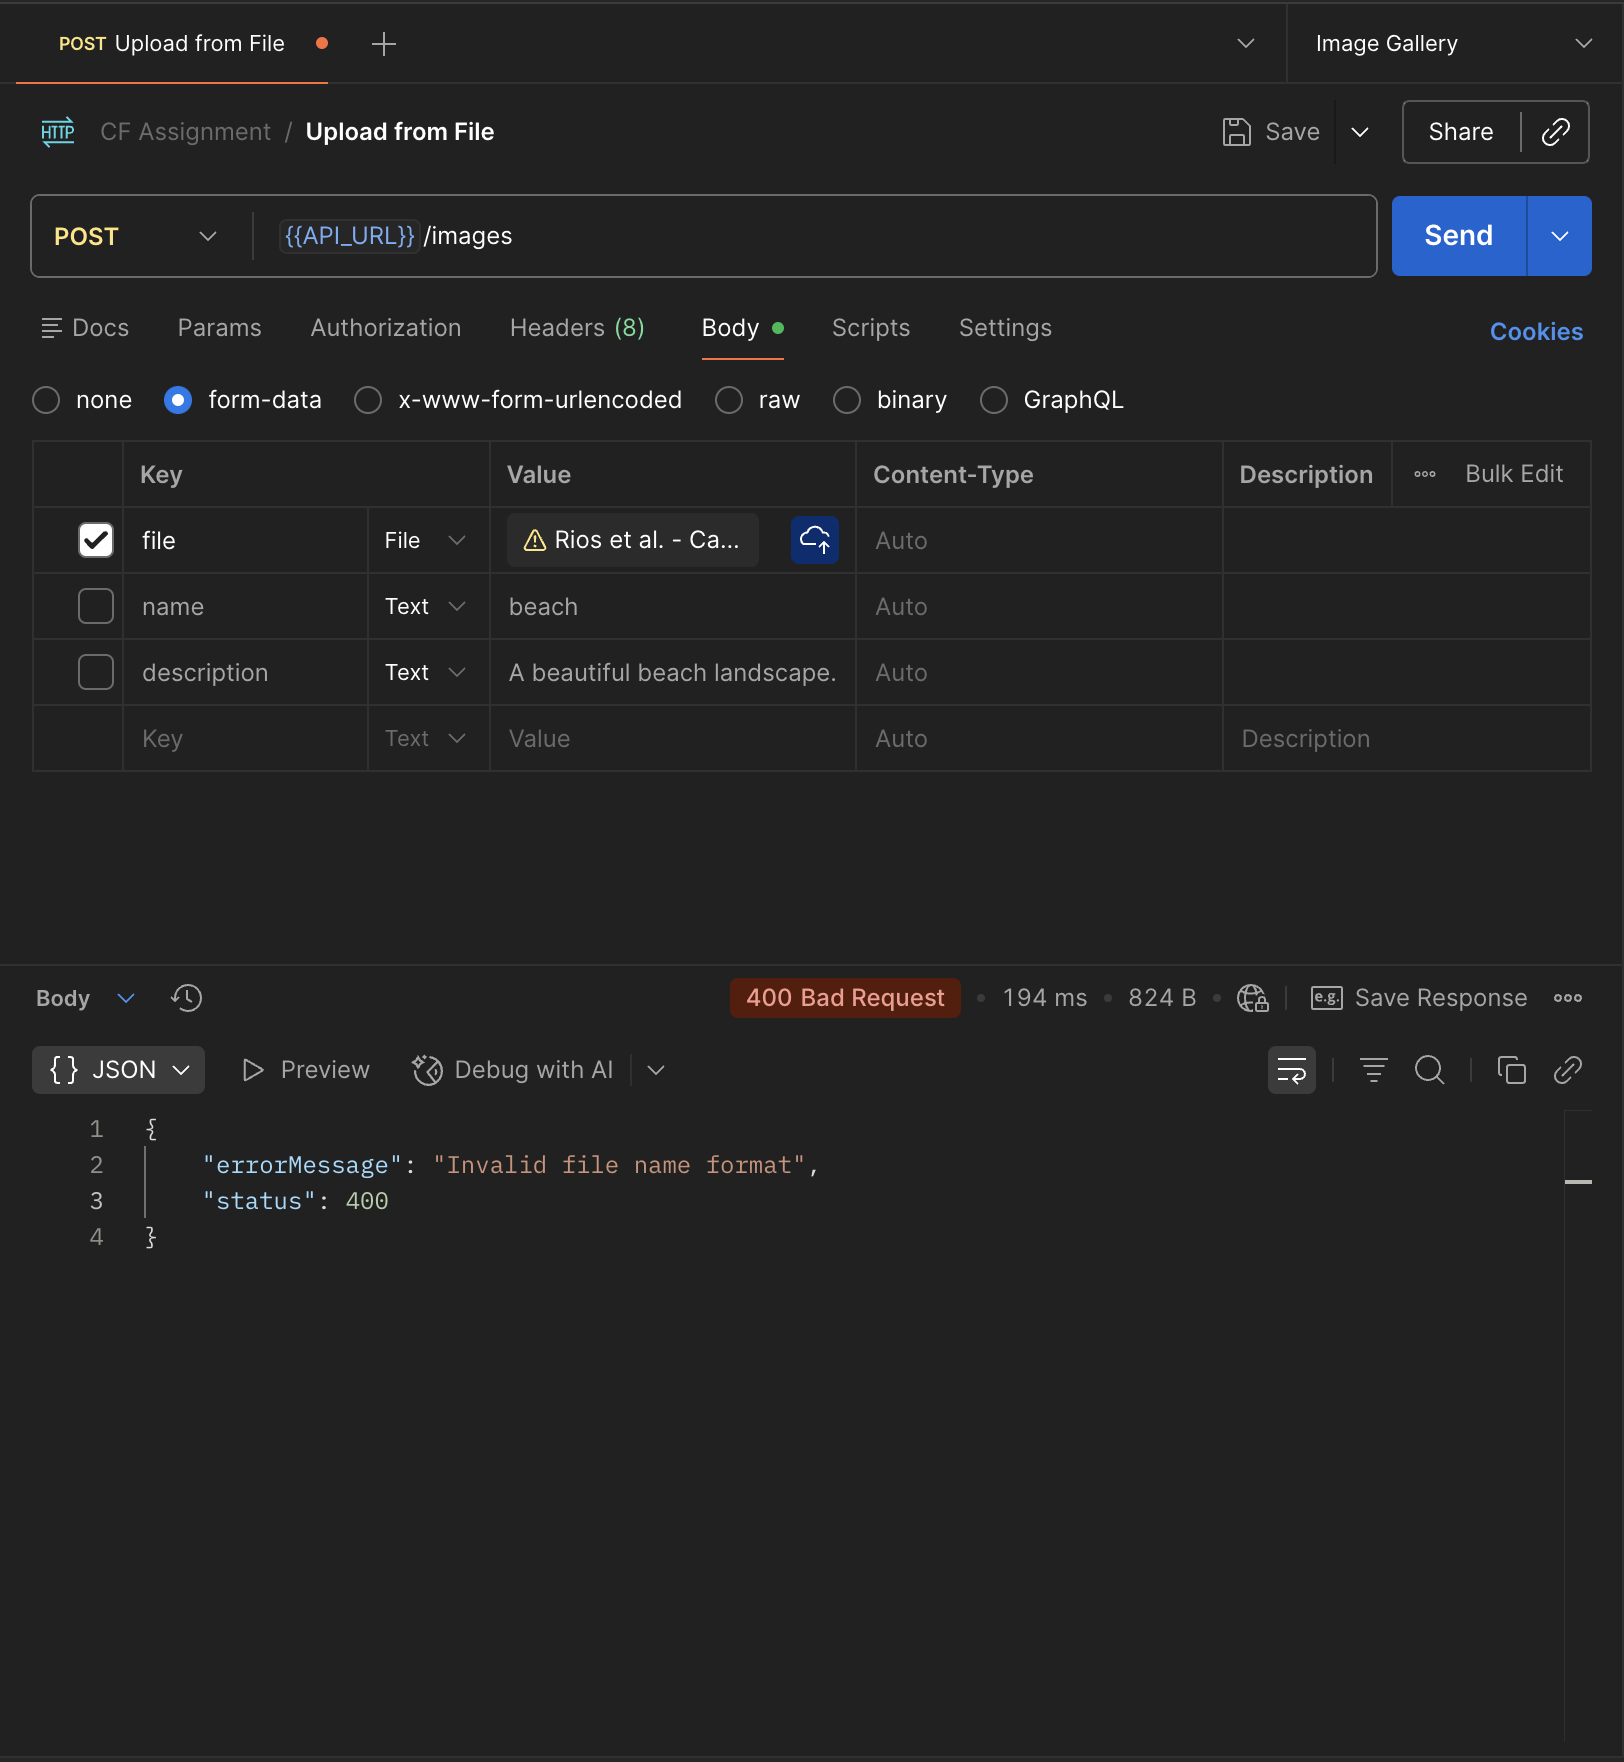
\includegraphics[width=\linewidth]{media/testing-evidence/upload-file-failure-bad-name.png}
\end{minipage}
\end{figure}

\subsection{Deleting Images}
Hit \texttt{DELETE https://image-gallery.goncalo2k.pt/images/:id}.

\subsubsection{Testing Evidence}

\begin{figure}[h]
\centering
\begin{minipage}{0.45\textwidth}
\centering
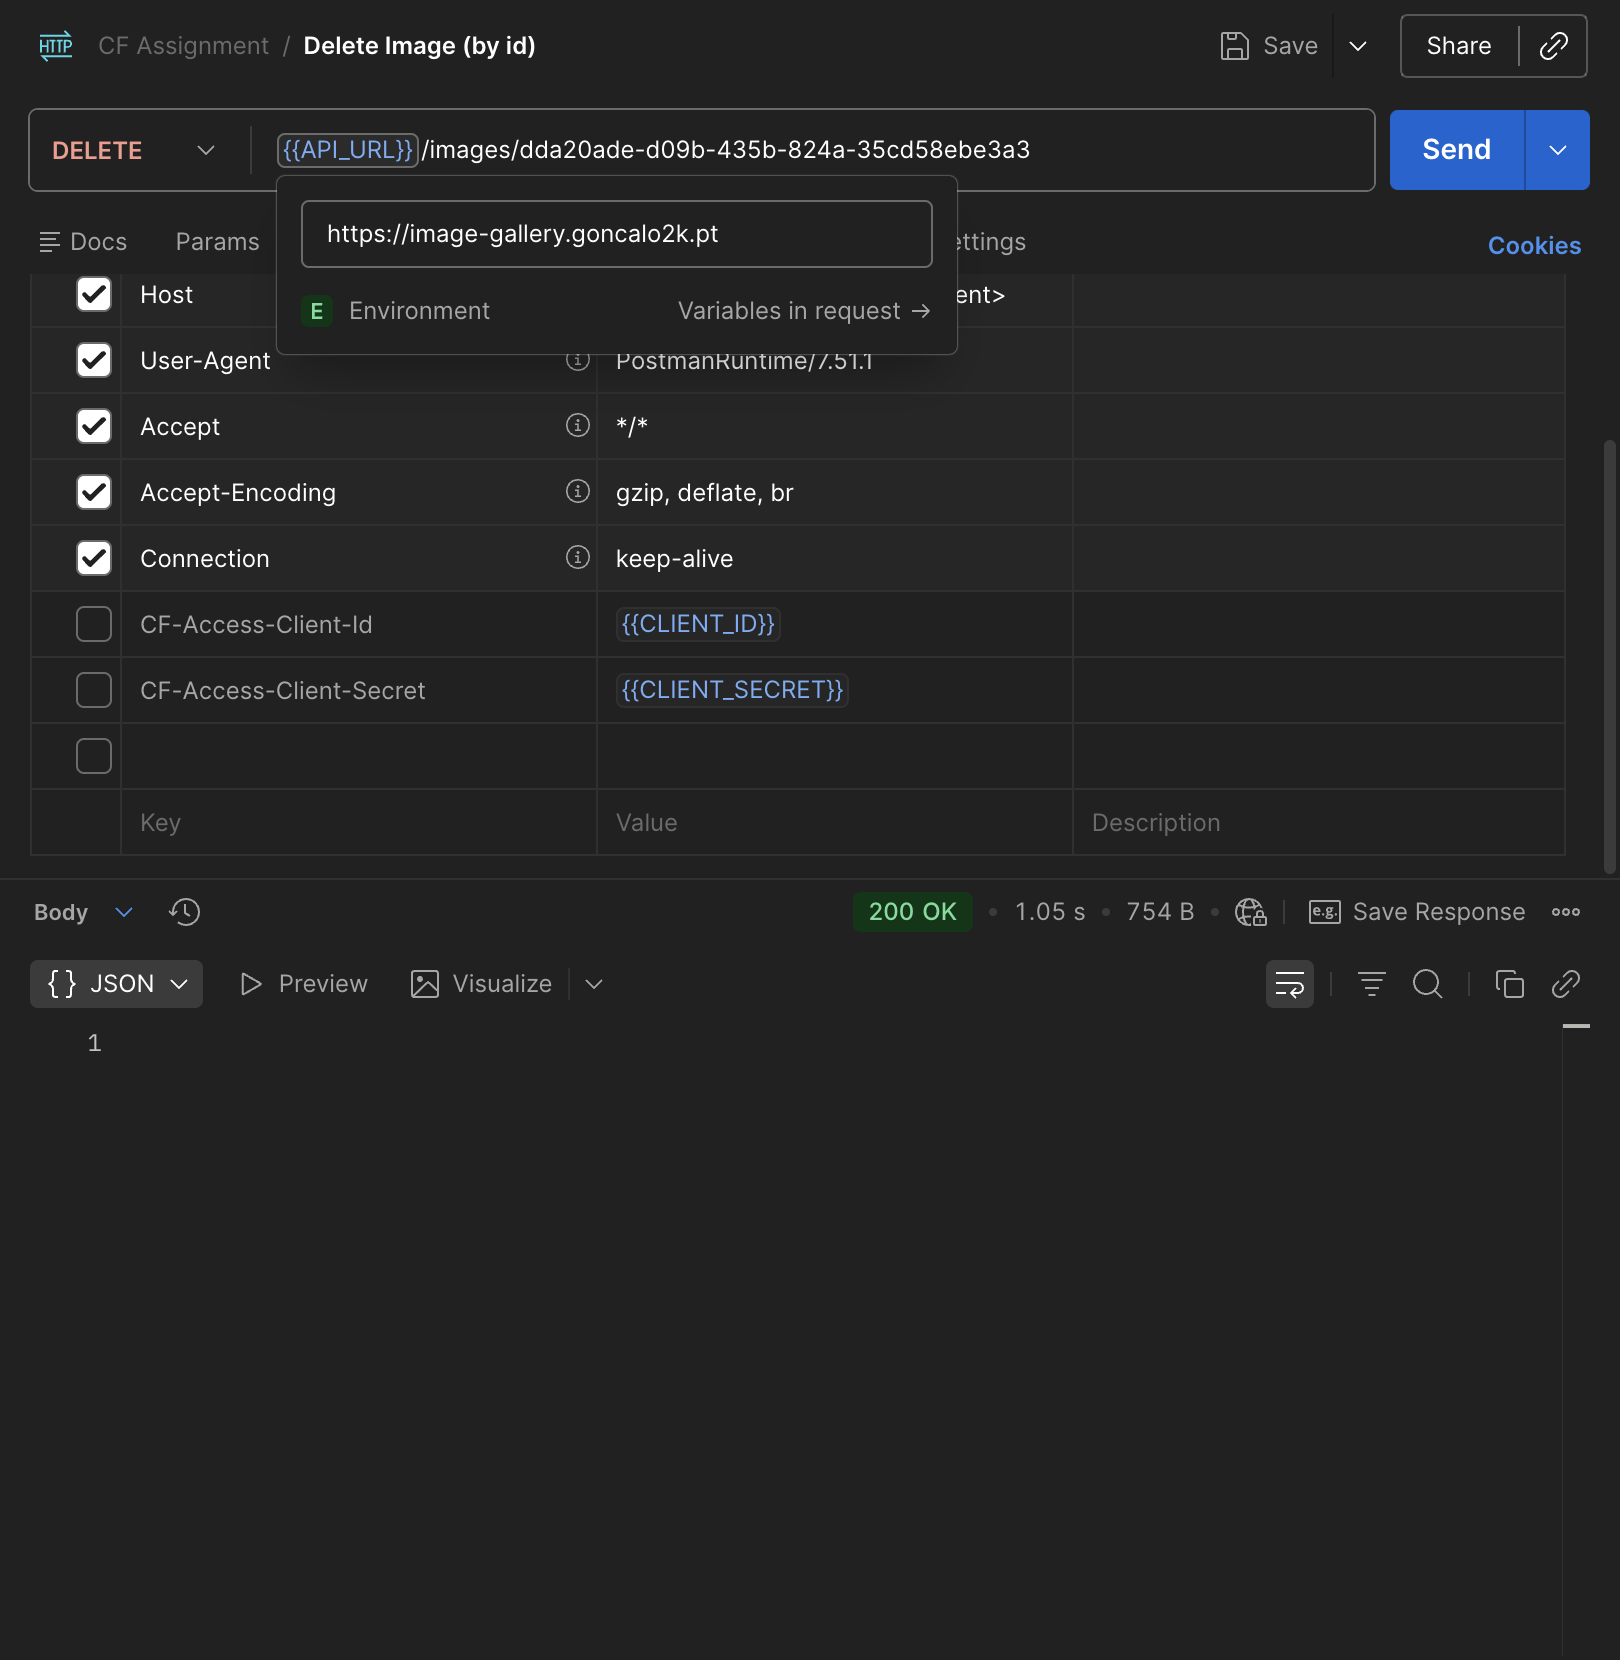
\includegraphics[width=\linewidth]{media/testing-evidence/delete-success.png}
\end{minipage}
\begin{minipage}{0.45\textwidth}
\centering
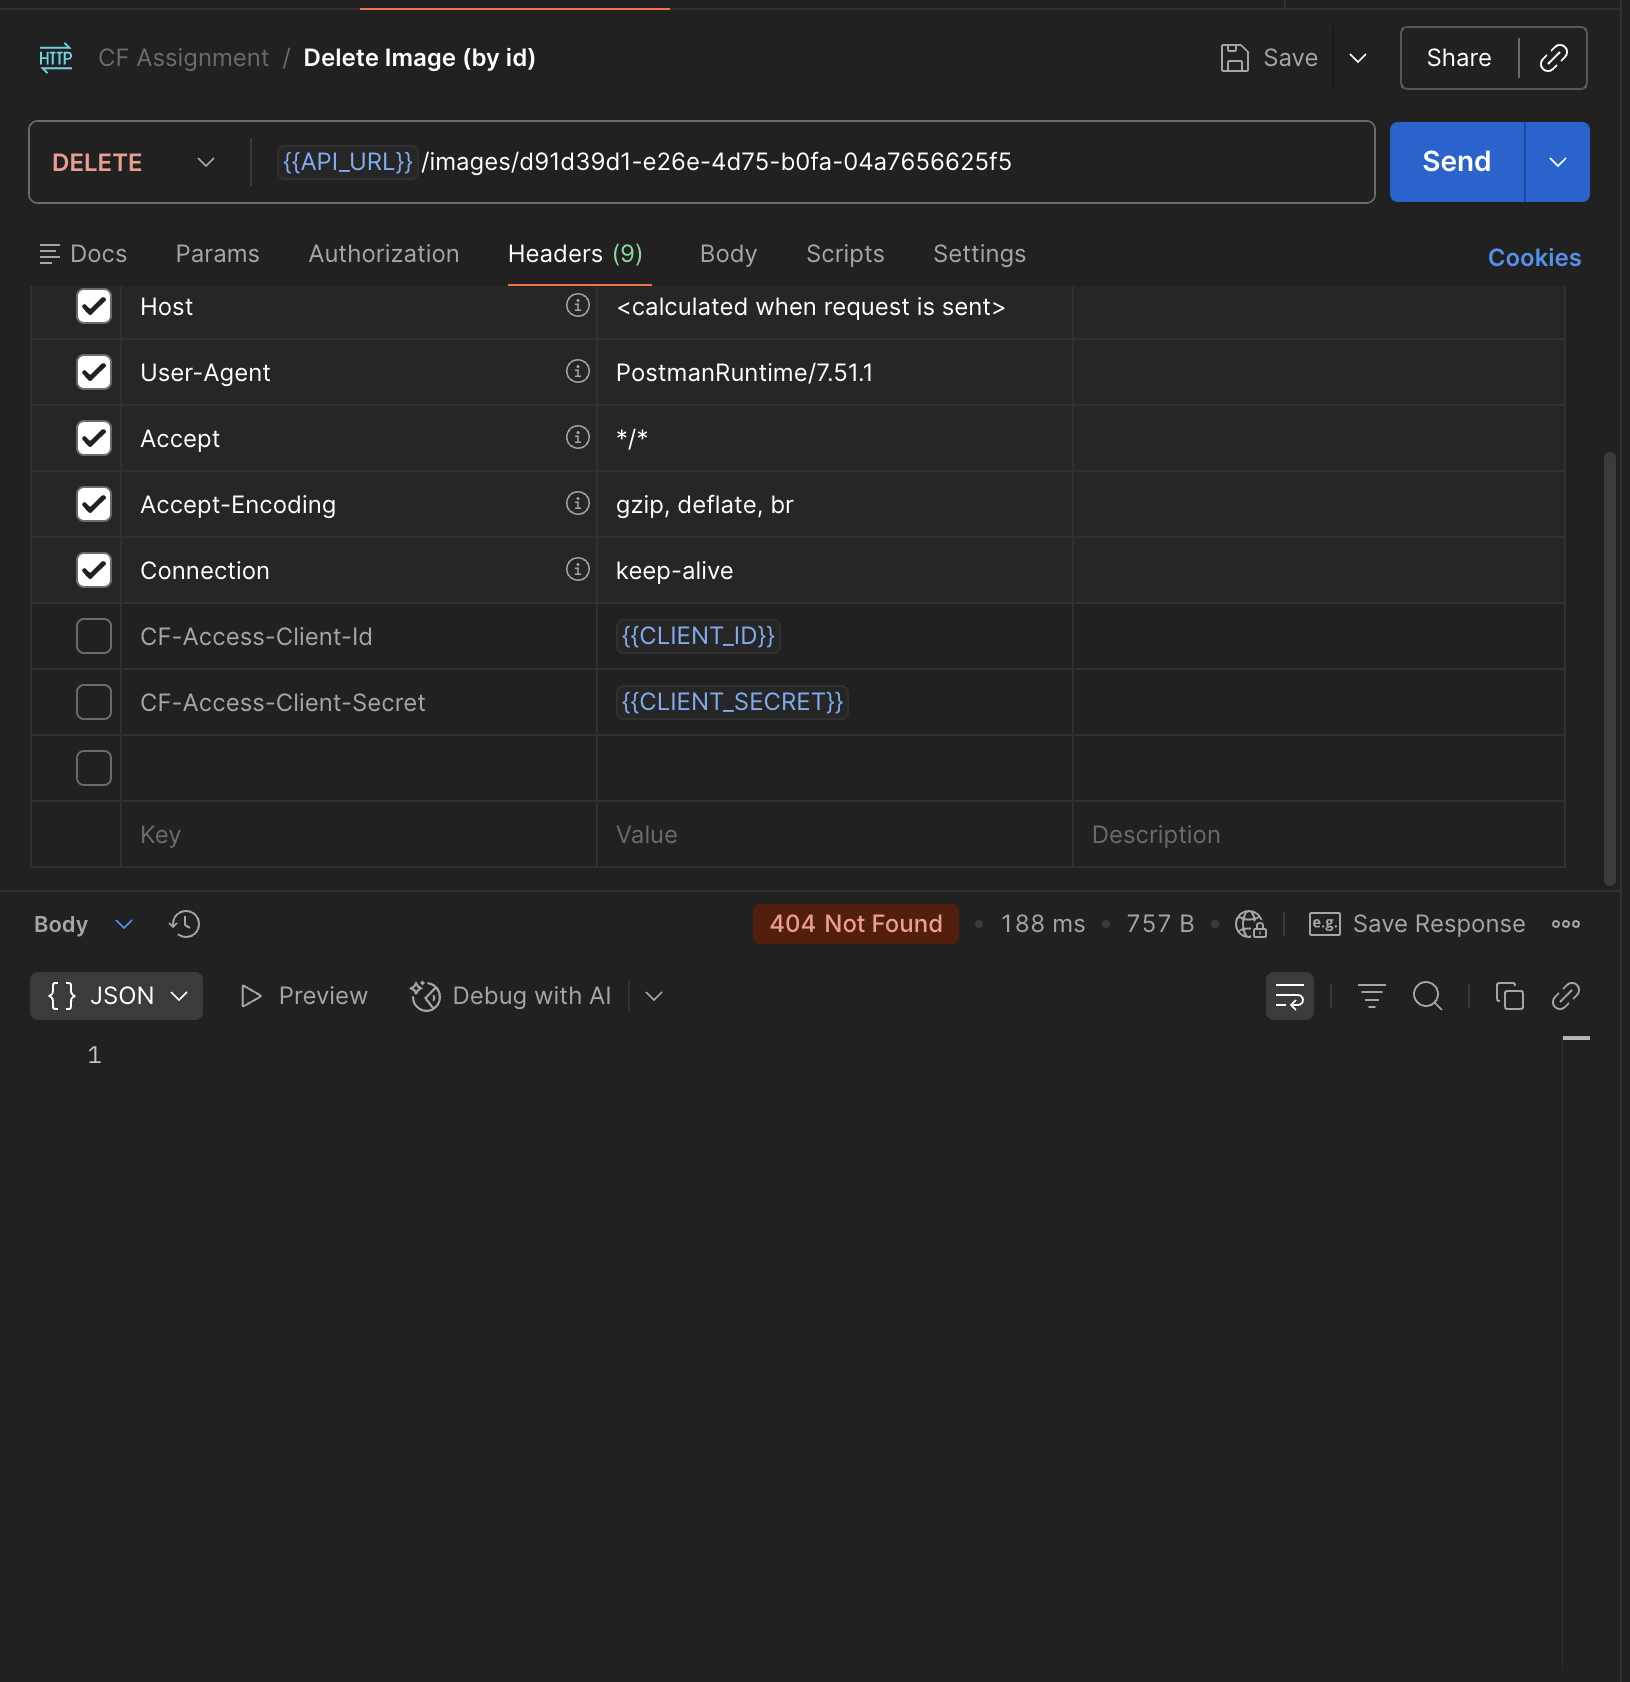
\includegraphics[width=\linewidth]{media/testing-evidence/delete-file-not-found.png}
\end{minipage}
\end{figure}

\subsection{Administrative Audit Endpoint}
Send \texttt{GET https://image-gallery.goncalo2k.pt/images/audit?offset=0\&limit=20} with the Access headers to retrieve recent uploads plus aggregate stats (\texttt{totalImages}, \texttt{lastUpdated}). Use this endpoint to populate dashboards or monitor image insertion or deletion. Note that this endpoint is also paginated.

\subsubsection{Testing evidence}

\begin{figure}[h]
\centering
\begin{minipage}{0.45\textwidth}
\centering
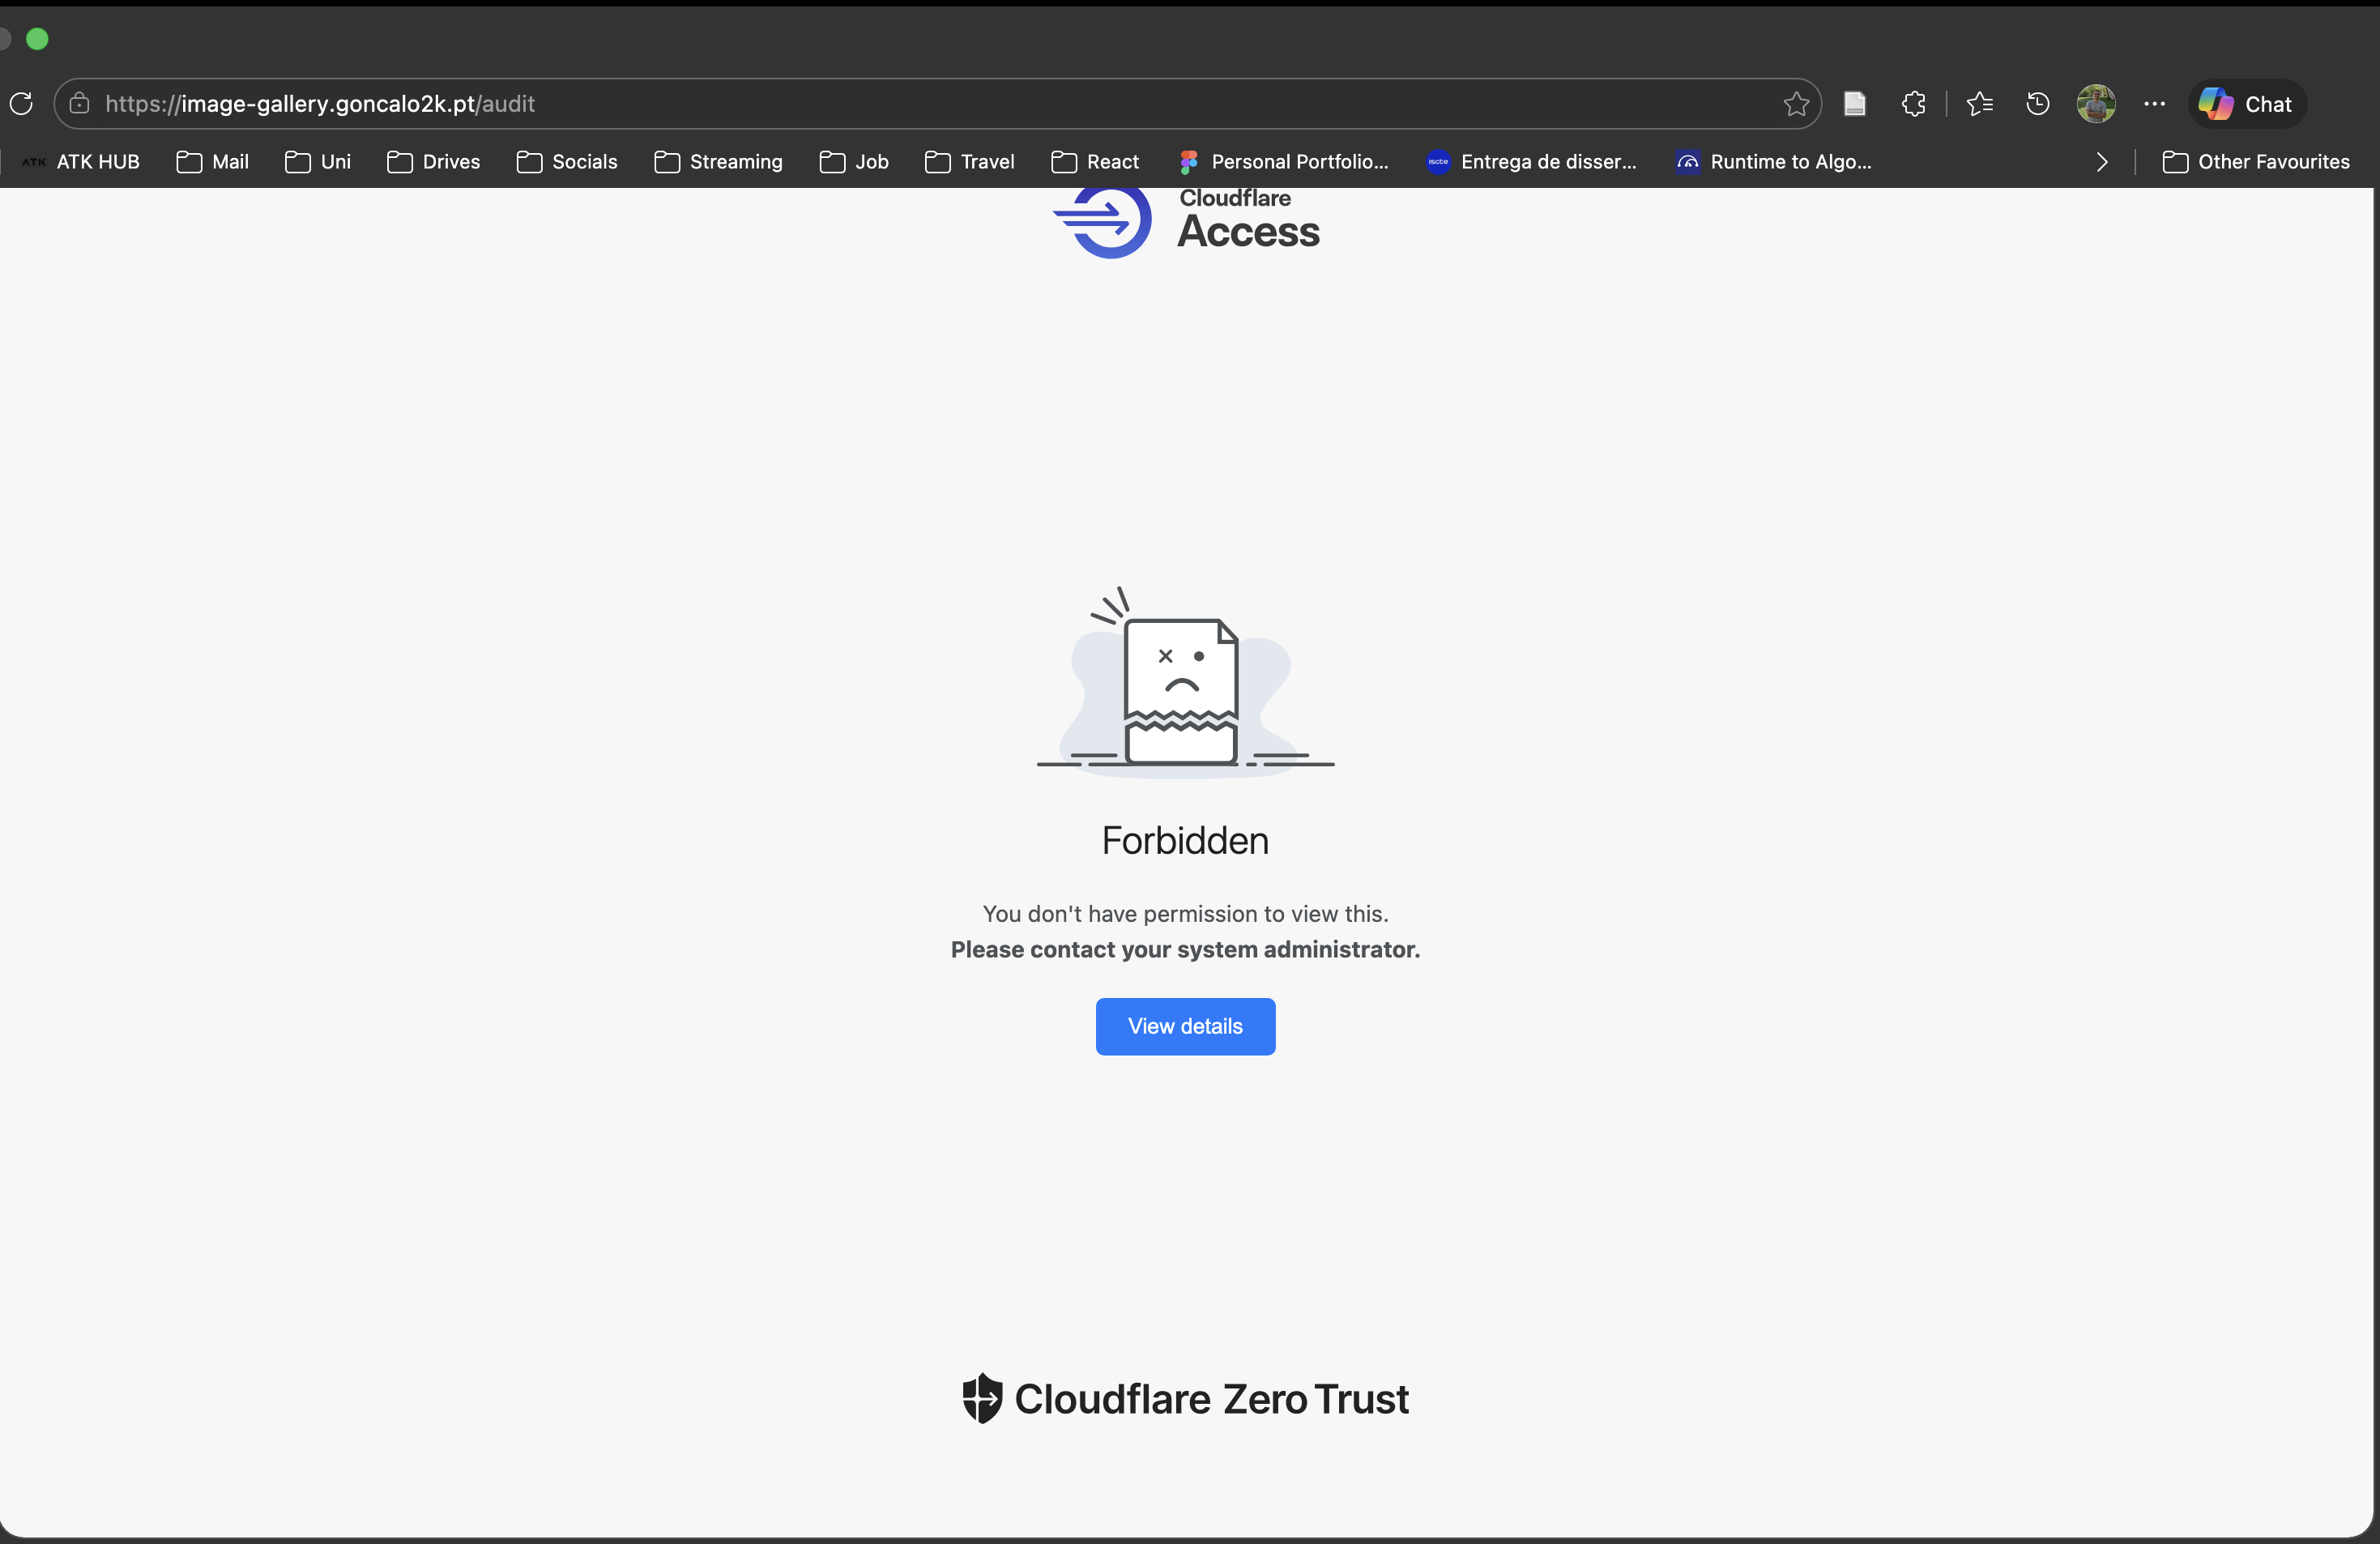
\includegraphics[width=\linewidth]{media/testing-evidence/audit-forbiden.png}
\end{minipage}
\begin{minipage}{0.45\textwidth}
\centering
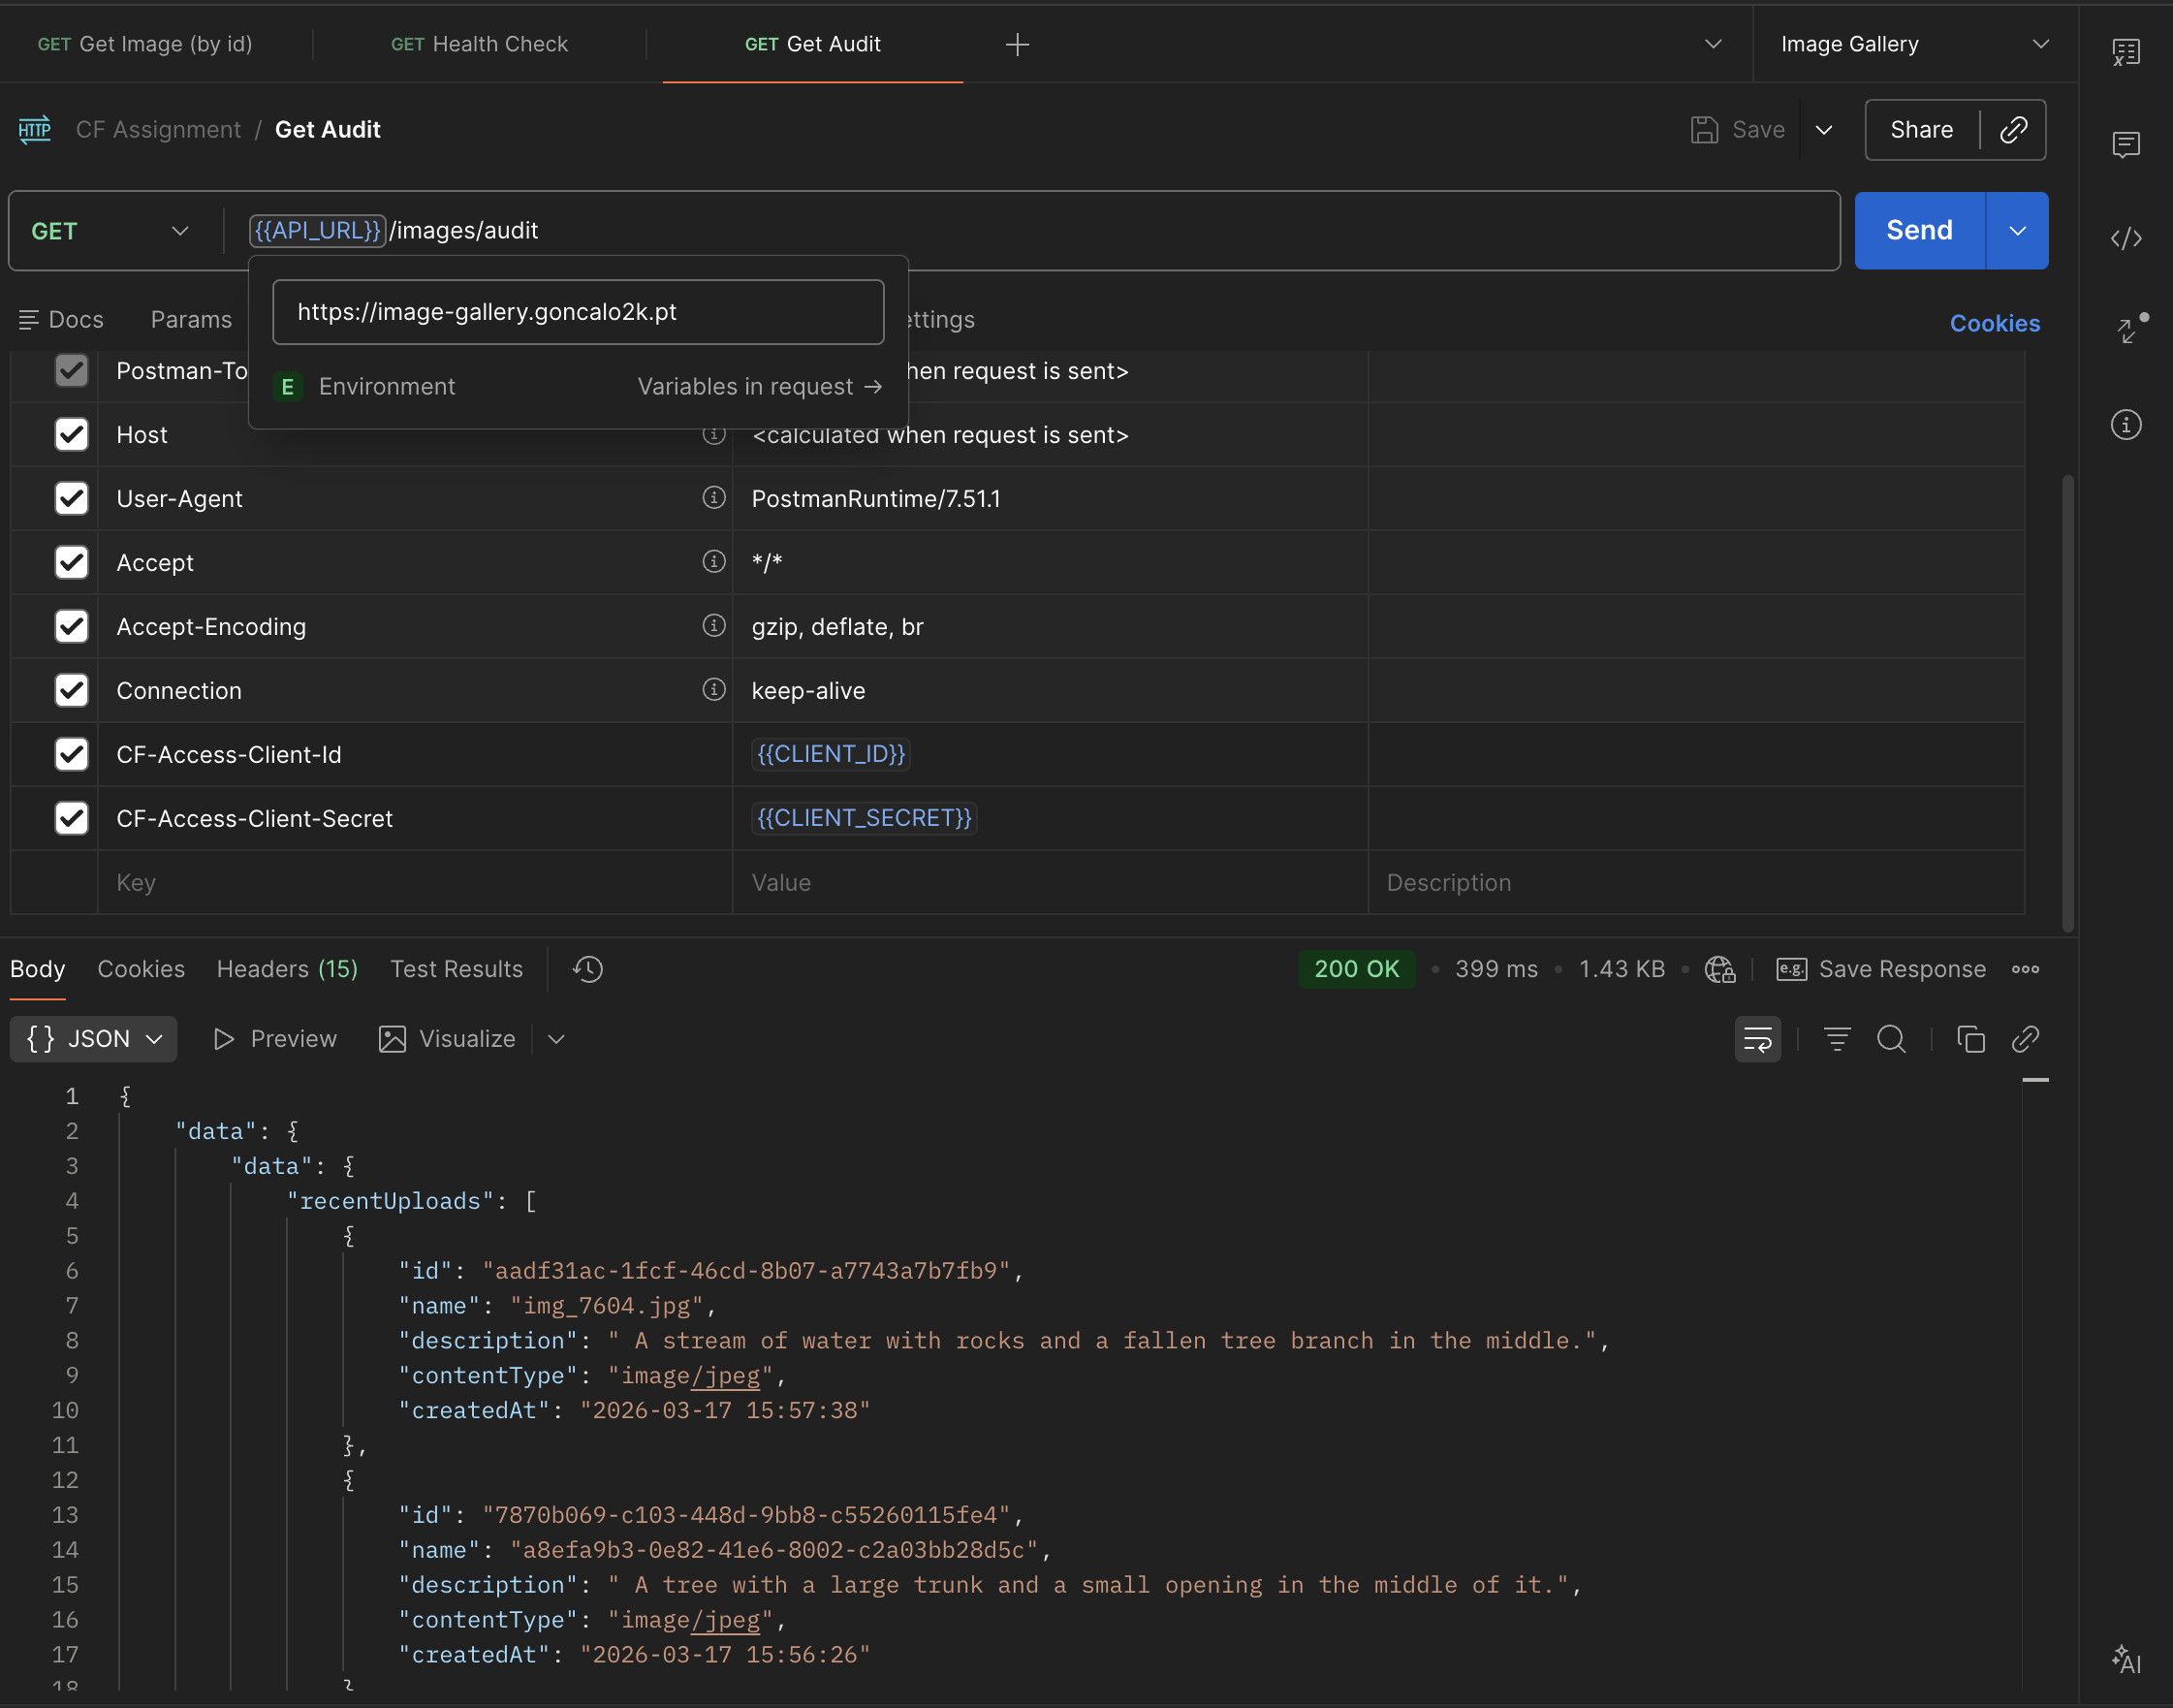
\includegraphics[width=\linewidth]{media/testing-evidence/audit-success.png}
\end{minipage}
\end{figure}

\section{Solution Architecture}
Image gallery was built as a combination of several Cloudflare-managed services that each handle a discrete responsibility while sharing data through Worker bindings and secure environment variables.

\subsection{System Components and Architecture}
\subsubsection{System Components}
\begin{itemize}[leftmargin=*]
  \item \textbf{R2 Object Storage} – Private bucket that stores the binary data for every upload. Workers never expose the bucket directly; all reads/writes go through bindings so IAM stays centralized.
  \item \textbf{Workers AI} – Generates descriptive alt text when the user does not provide one. Requests are throttled by resizing buffers first to stay within inference limits.
  \item \textbf{D1 Database} – Holds authoritative metadata (name, description, MIME type, timestamps). Lookups prevent duplicate uploads and feed \texttt{/images}, \texttt{/images/audit}, and delete checks.
  \item \textbf{Cache API} – Provides immutable edge caching for \texttt{GET /images/:id}. Deletes schedule cache invalidation via \texttt{executionCtx.waitUntil} to keep replicas in sync.
  \item \textbf{Cloudflare Access} – Protects \texttt{/images/audit} (and any future admin route) with service tokens enforced by \texttt{auth.middleware.ts}.
  \item \textbf{Cloudflare Images} – Acts as an on-the-fly transformer so Workers AI receives 1024×1024 JPEGs even when creators upload multi‑megabyte PNGs.
\end{itemize}

\subsubsection{High-level System Architecture}

The worker sits at the center of the platform and orchestrates multiple services: R2 stores every uploaded binary, Workers AI produces fallback descriptions, D1 keeps normalized metadata, Cloudflare Images resizes large buffers before inference, and the Cache API accelerates read-heavy endpoints. Cloudflare Access service tokens wrap the privileged \texttt{/images/audit} route behind Zero-Trust authentication while environment secrets keep every credential outside the codebase. Each upload request streams the file into R2, generates or reuses alt text, and enqueues a metadata write in D1; download requests hydrate cache entries with immutable headers so subsequent requests are answered directly from Cloudflare’s edge. Supporting scripts (batch upload + clear) exercise the same public endpoints which means operational automation never bypasses access controls. The diagram below captures how those building blocks interact at runtime.

\begin{center}
  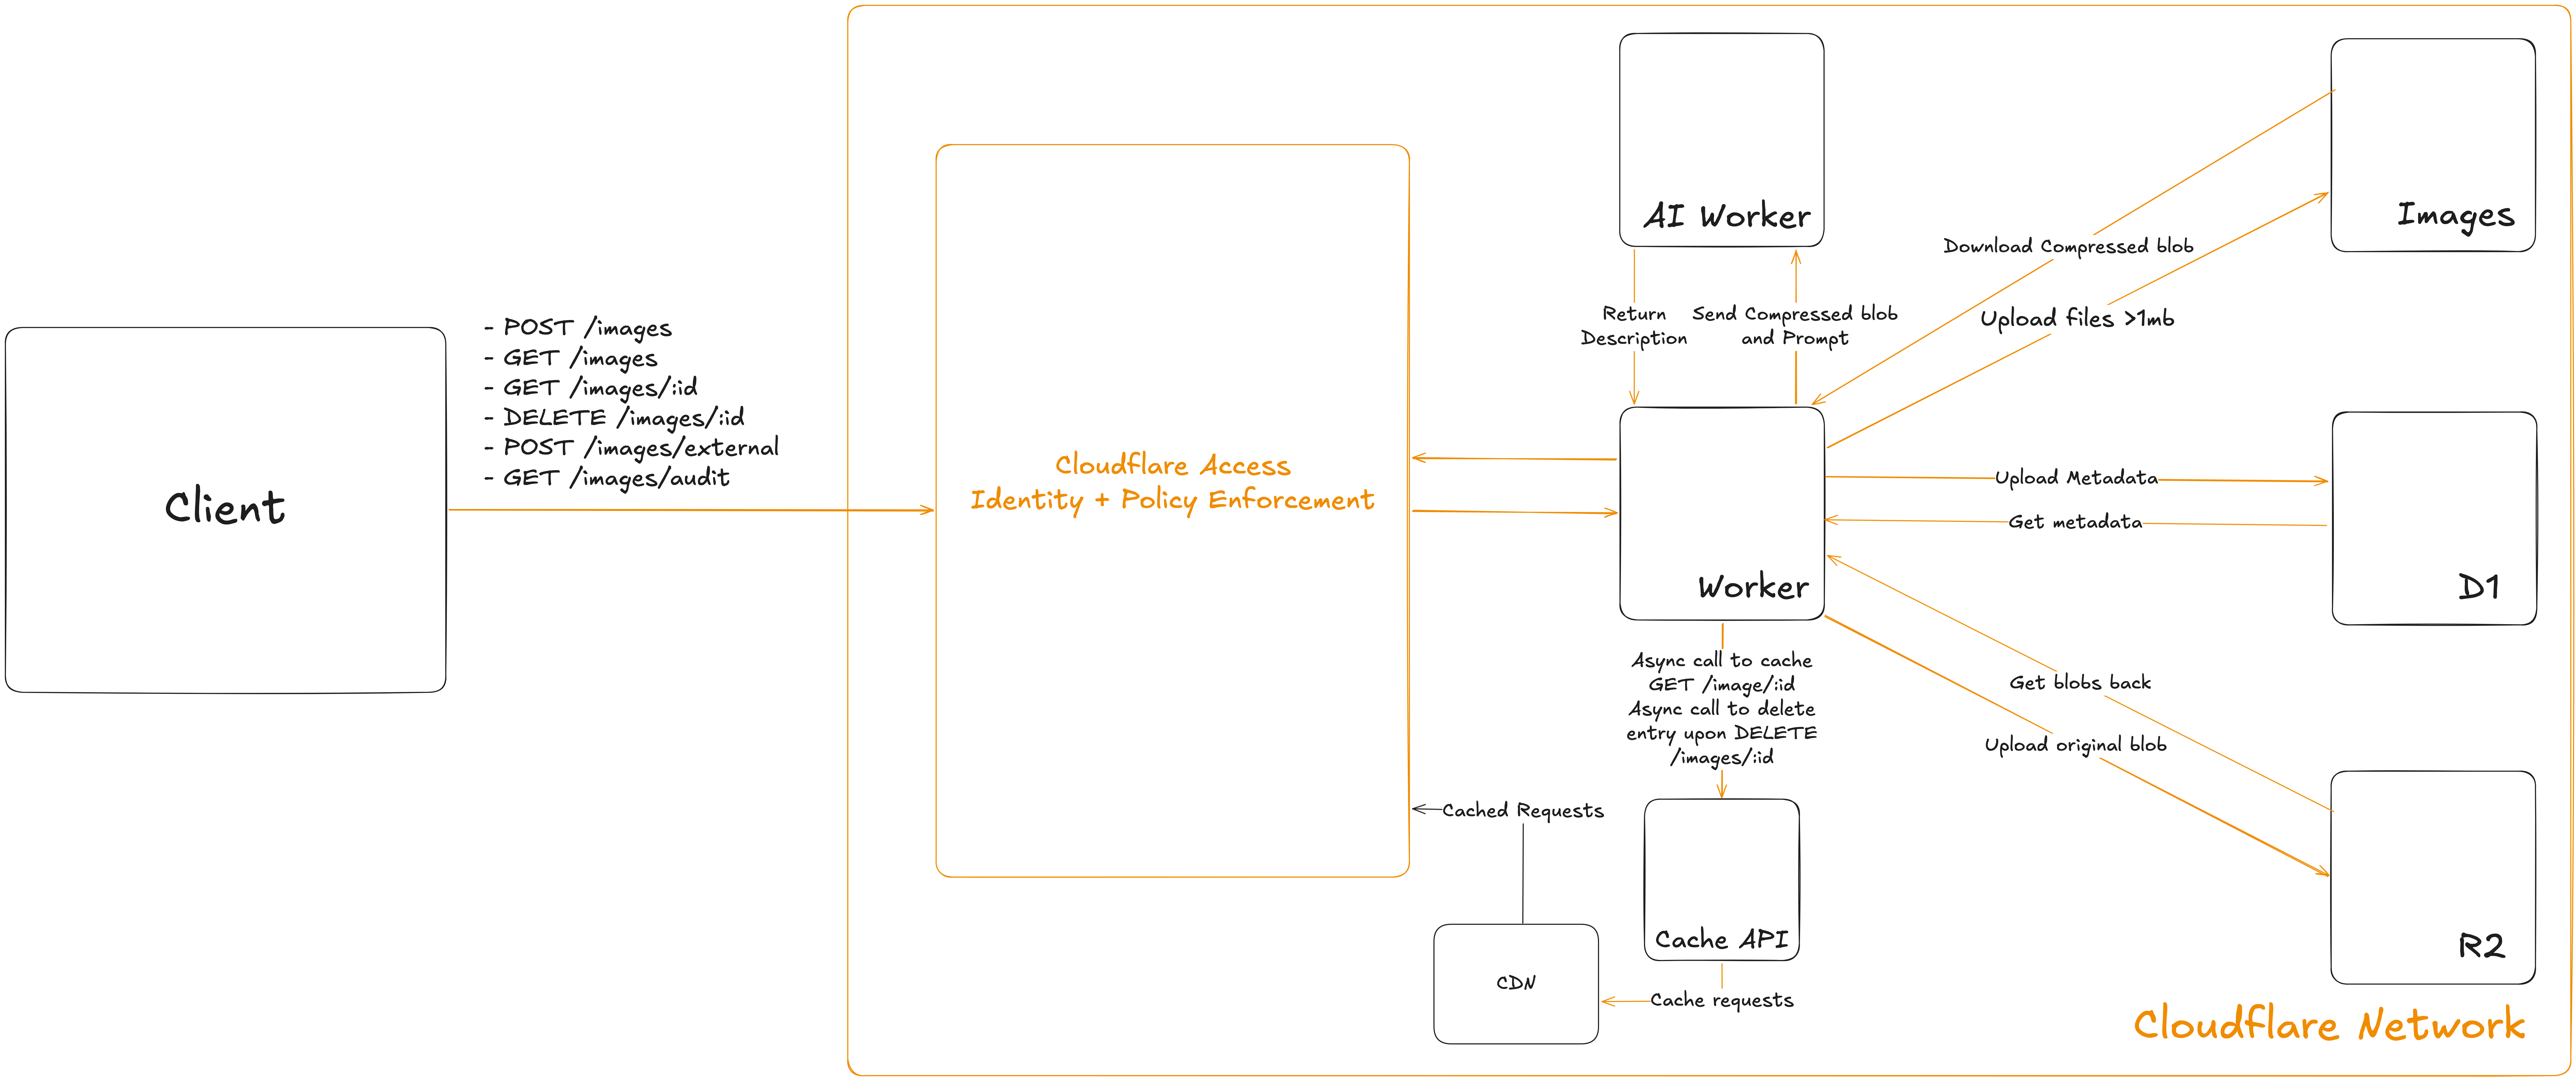
\includegraphics[width=0.85\textwidth]{diagrams/system-architecture-diagram.png}
\end{center}

\subsubsection{High-level Worker Architecture}

The Framework utilzed to build the worker was Hono, as it is compatible with Cloudflare out-of-the-box and very lightweight, which sped up the delivery process.

From a code perspective, \texttt{src/app.ts} wires the Hono router together with middleware for logging, CORS, authentication, and security headers so every request flows through a consistent envelope. \texttt{routes/image.routes.ts} mounts the controller methods under \texttt{/images}, while \texttt{ImageController} focuses on HTTP concerns such as parsing payloads, caching R2 responses, invalidating cache entries after deletes, and translating service results into JSON bodies. The heavy lifting lives in \texttt{ImageService}: it validates filenames and MIME types, streams uploads to R2, generates alt text with Workers AI (resizing buffers via the Images binding when necessary), inserts metadata into D1, fetches audit logs, and runs deletion fan‑out across R2 and D1 in parallel. Utility modules (\texttt{image-mapper}, \texttt{utils/utils.ts}) provide reusable helpers for pagination, CSV/env parsing, and DTO transformations so controllers and services stay small. Middleware round things out: \texttt{auth.middleware.ts} protects configured routes with timing-safe header comparisons, \texttt{logger-middleware.ts} attaches correlation IDs plus structured logs, \texttt{cors.middleware.ts} enforces allow-lists, and \texttt{security-headers.middleware.ts} emits CSP/nosniff defaults. Tests under \texttt{src/**/*.spec.ts} exercise each layer, giving rapid feedback when iterating on the worker logic. This can be shown in the following diagram

\begin{center}
  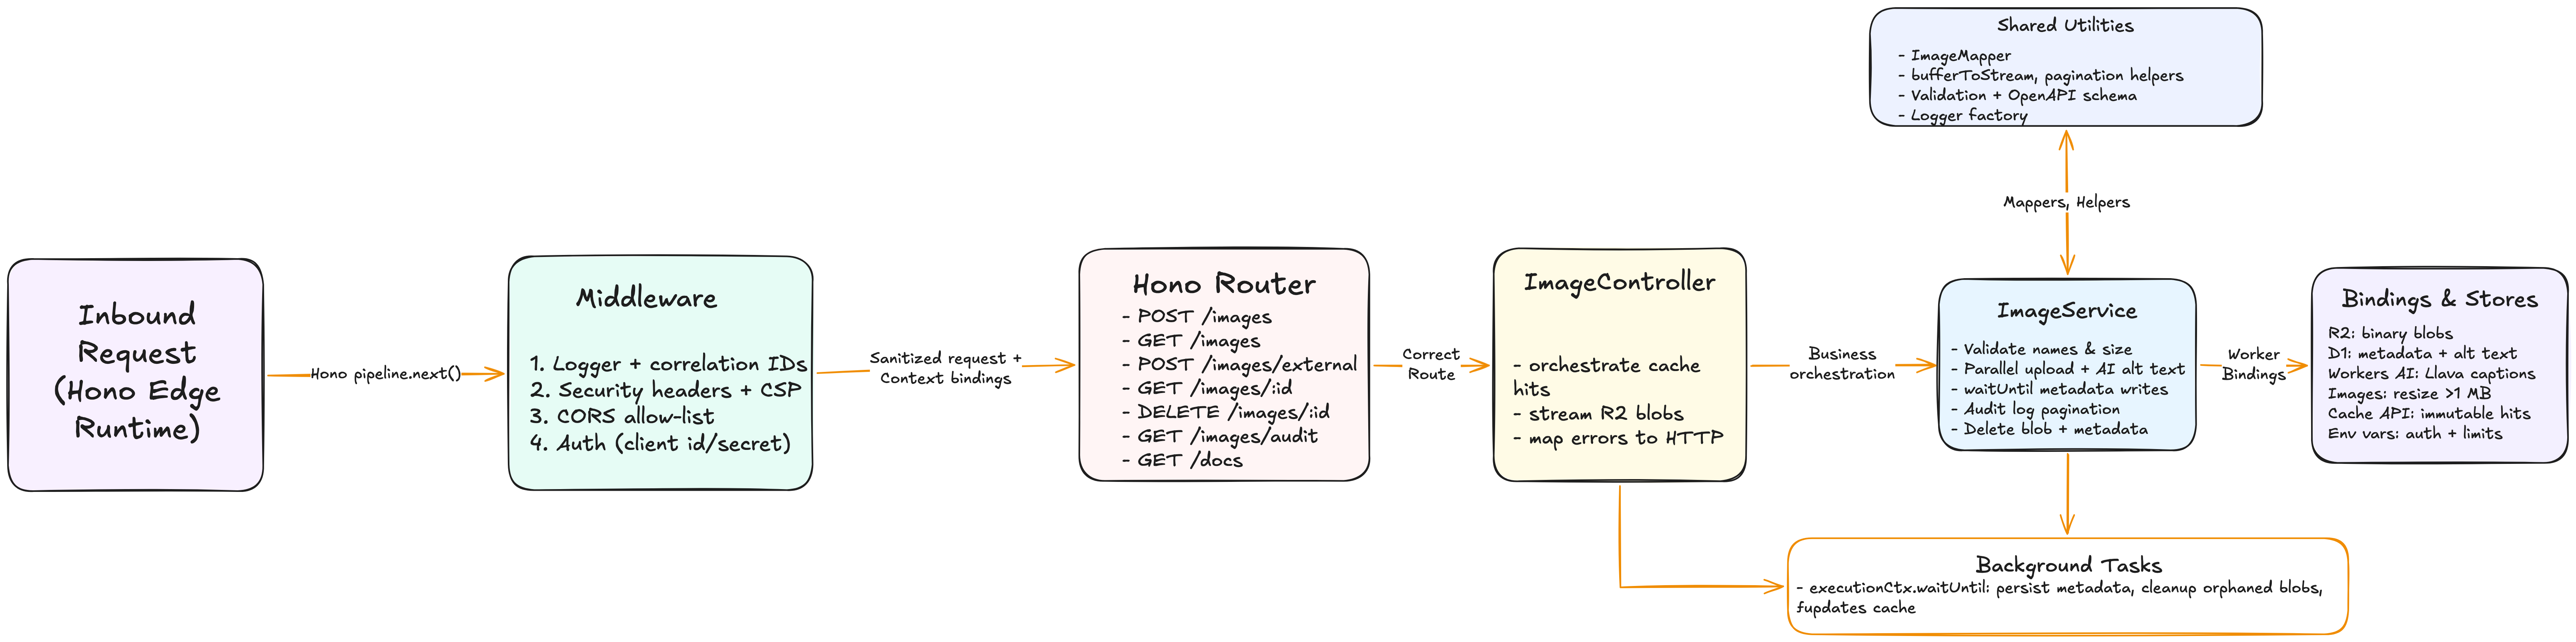
\includegraphics[width=0.9\textwidth]{diagrams/worker-high-level-design.png}
\end{center}

\section{Implementation}
The creation of building blocks was developed

\subsection{Prerequisites:}
\begin{enumerate}[leftmargin=*]
  \item Sign up for a \href{https://dash.cloudflare.com/}{Cloudflare Account}
  \item Install \href{https://docs.npmjs.com/downloading-and-installing-node-js-and-npm}{Node.js}
\end{enumerate}

\subsection{Worker Creation}
\begin{enumerate}[leftmargin=*]
  \item Install Wrangler CLI\\\texttt{pnpm i wrangler@latest}
  \item Login using Wrangler CLI\\\texttt{wrangler login}
  \item Create a worker using Wrangler CLI\\\texttt{pnpm create cloudflare@latest image-gallery}
  \item Select the directory where the project is going to be stored, select \textbf{Framework Starter} and then \textbf{Hono} as the framework.
  \item Enable Git for version control and deploy your worker.
  \item Finally, if the worker is supposed to be hosted on a custom domain, add the following lines to your \texttt{wrangler.jsonc}:\\\texttt{"routes": [\{ "pattern": "image-gallery.goncalo2k.pt", "custom\_domain": true \}\ ]}
\end{enumerate}

\subsection{R2 and D1 Creation}
\begin{enumerate}[leftmargin=*]
  \item Create D1 Database using Wrangler\\\texttt{npx wrangler@latest d1 create analogs-db}
  \item Create R2 Blob Storage using Wrangler\\\texttt{npx wrangler r2 bucket create analogs}
  \item Login to \href{https://dash.cloudflare.com}{Cloudflare Dashboard}
  \item Go to the \textbf{Storage} section, look for R2 and select your bucket.
  \item Disable public access for your bucket.\\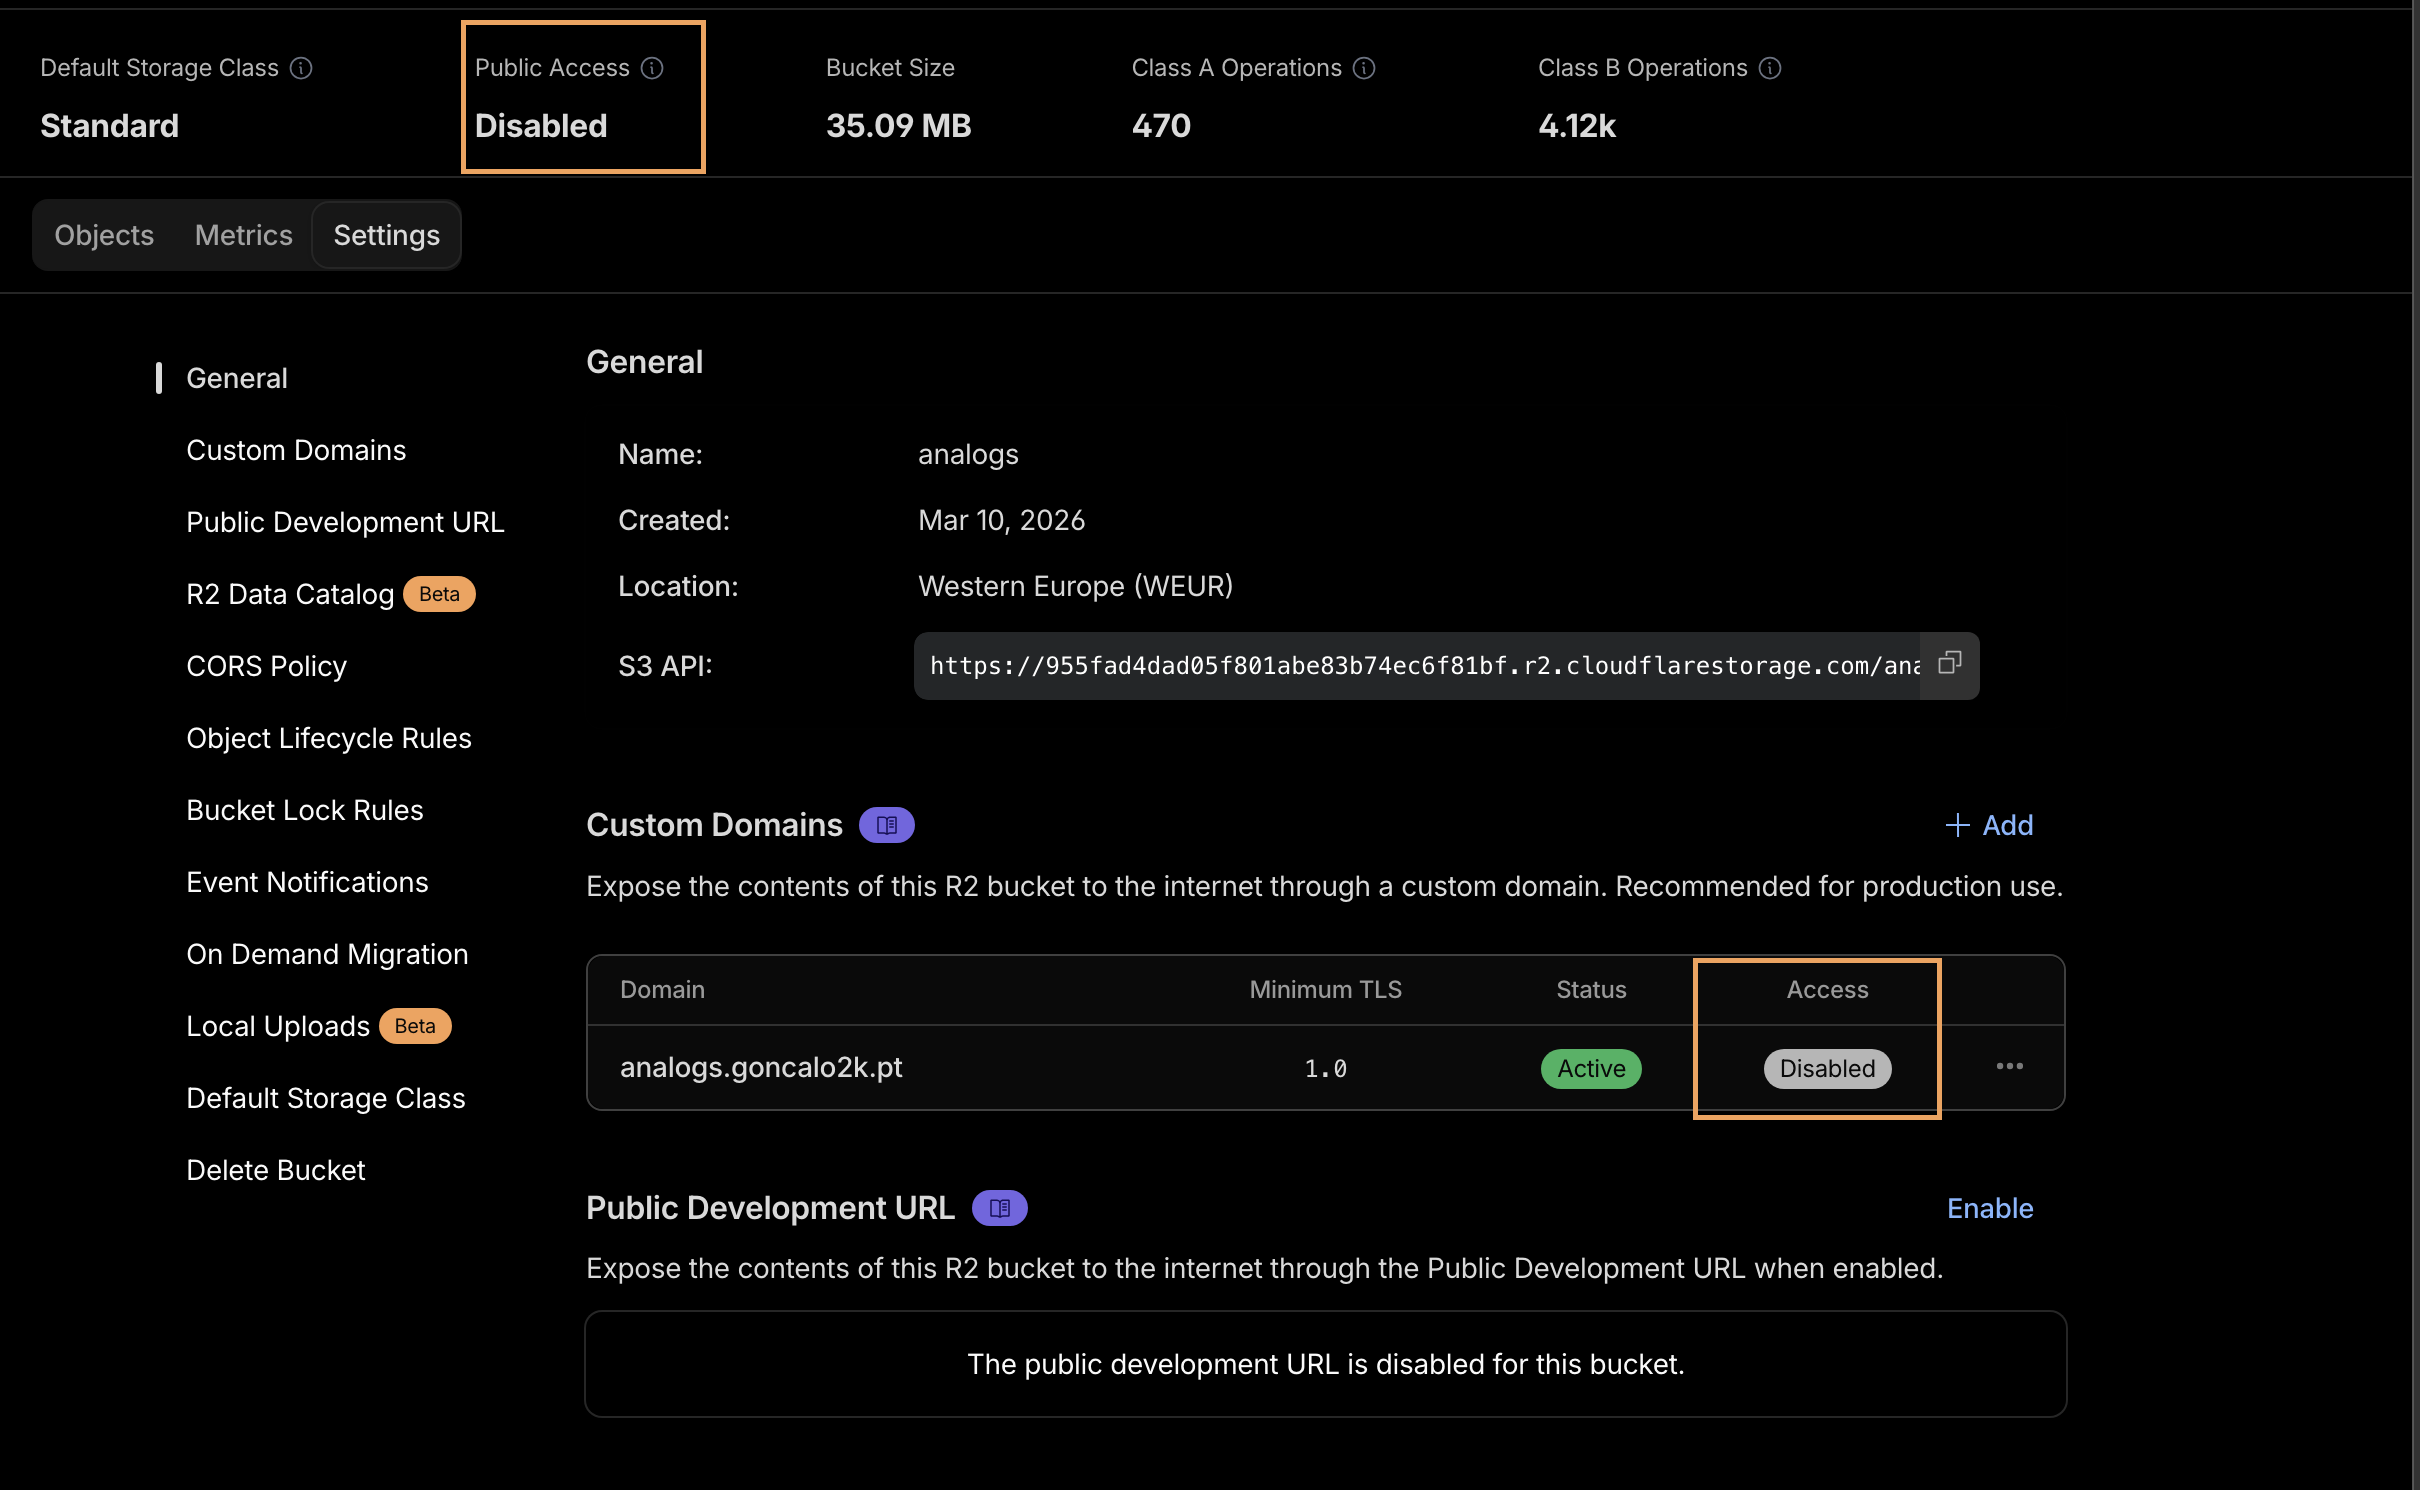
\includegraphics[width=0.6\textwidth]{media/r2/r2_security.png}
\end{enumerate}

\subsection{Service Token Creation}
\begin{enumerate}[leftmargin=*]
  \item Login to \href{https://dash.cloudflare.com}{Cloudflare Dashboard}
  \item Go to \textbf{Zero Trust}, \textbf{Access Controls} and then \textbf{Service Credentials}
  \item Select \textbf{Create Service Token}\\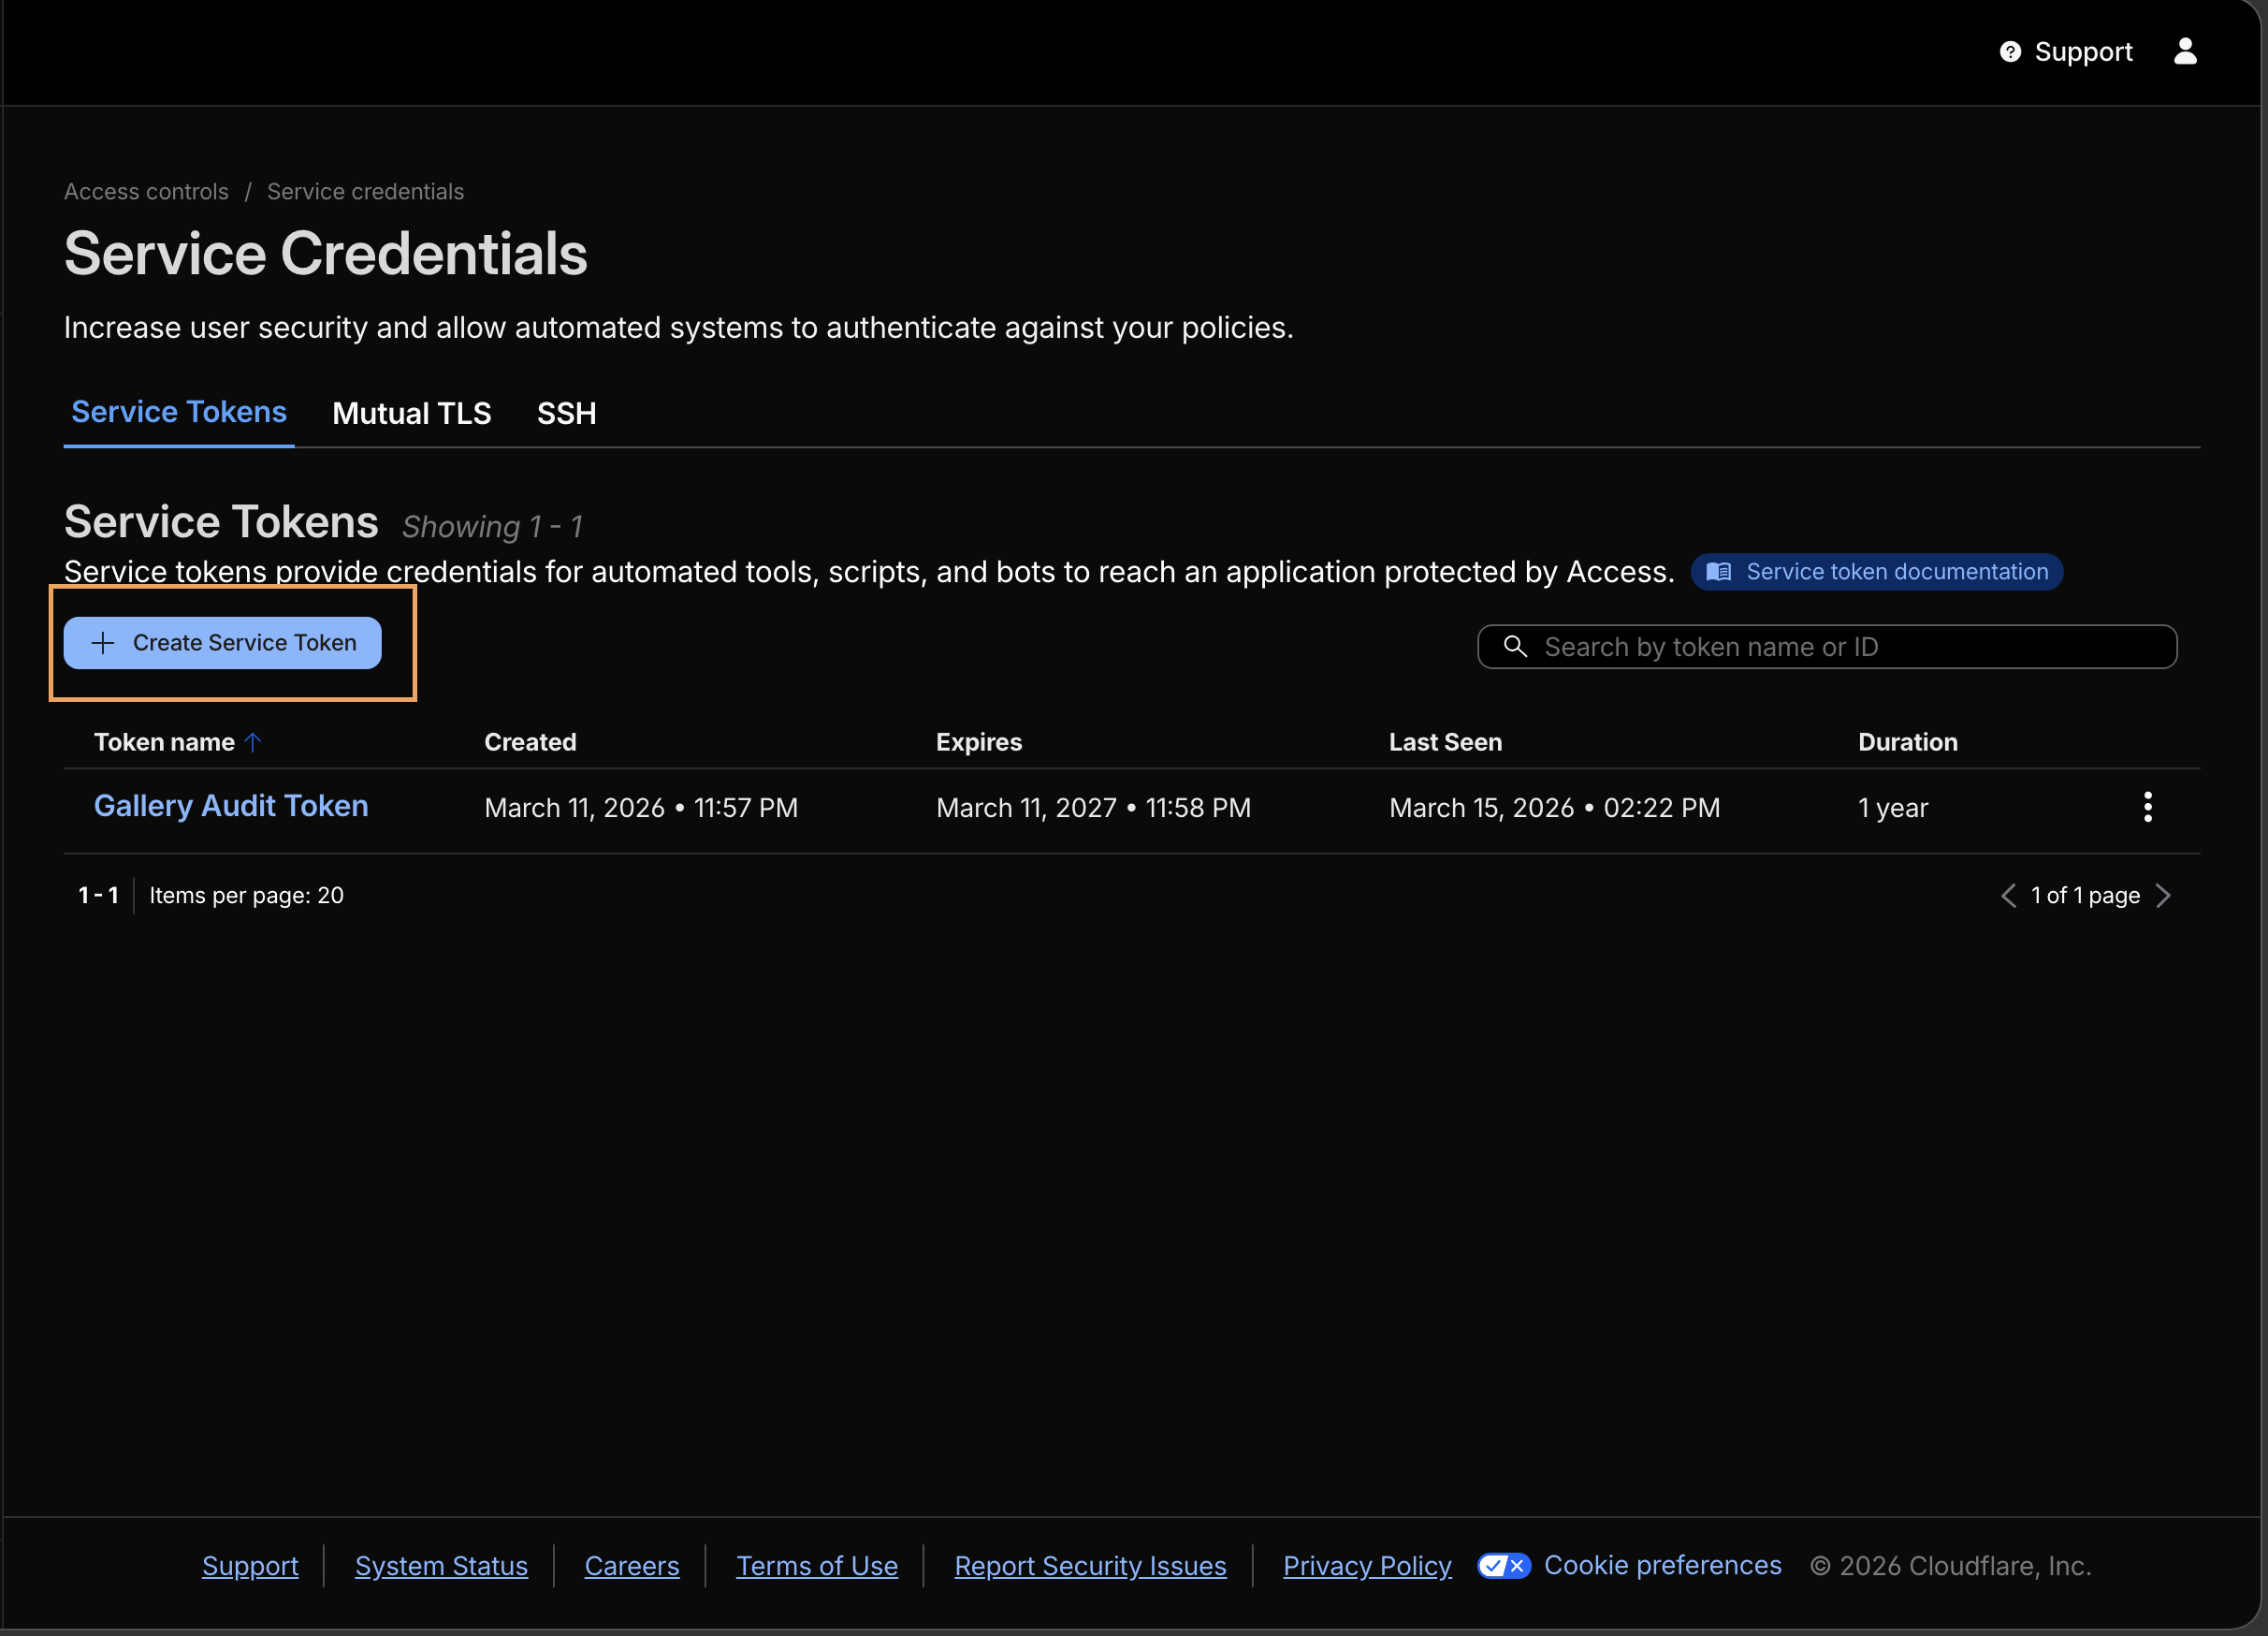
\includegraphics[width=0.5\textwidth]{media/token/token_1.png}
  \item Add a name and a token duration, then generate it\\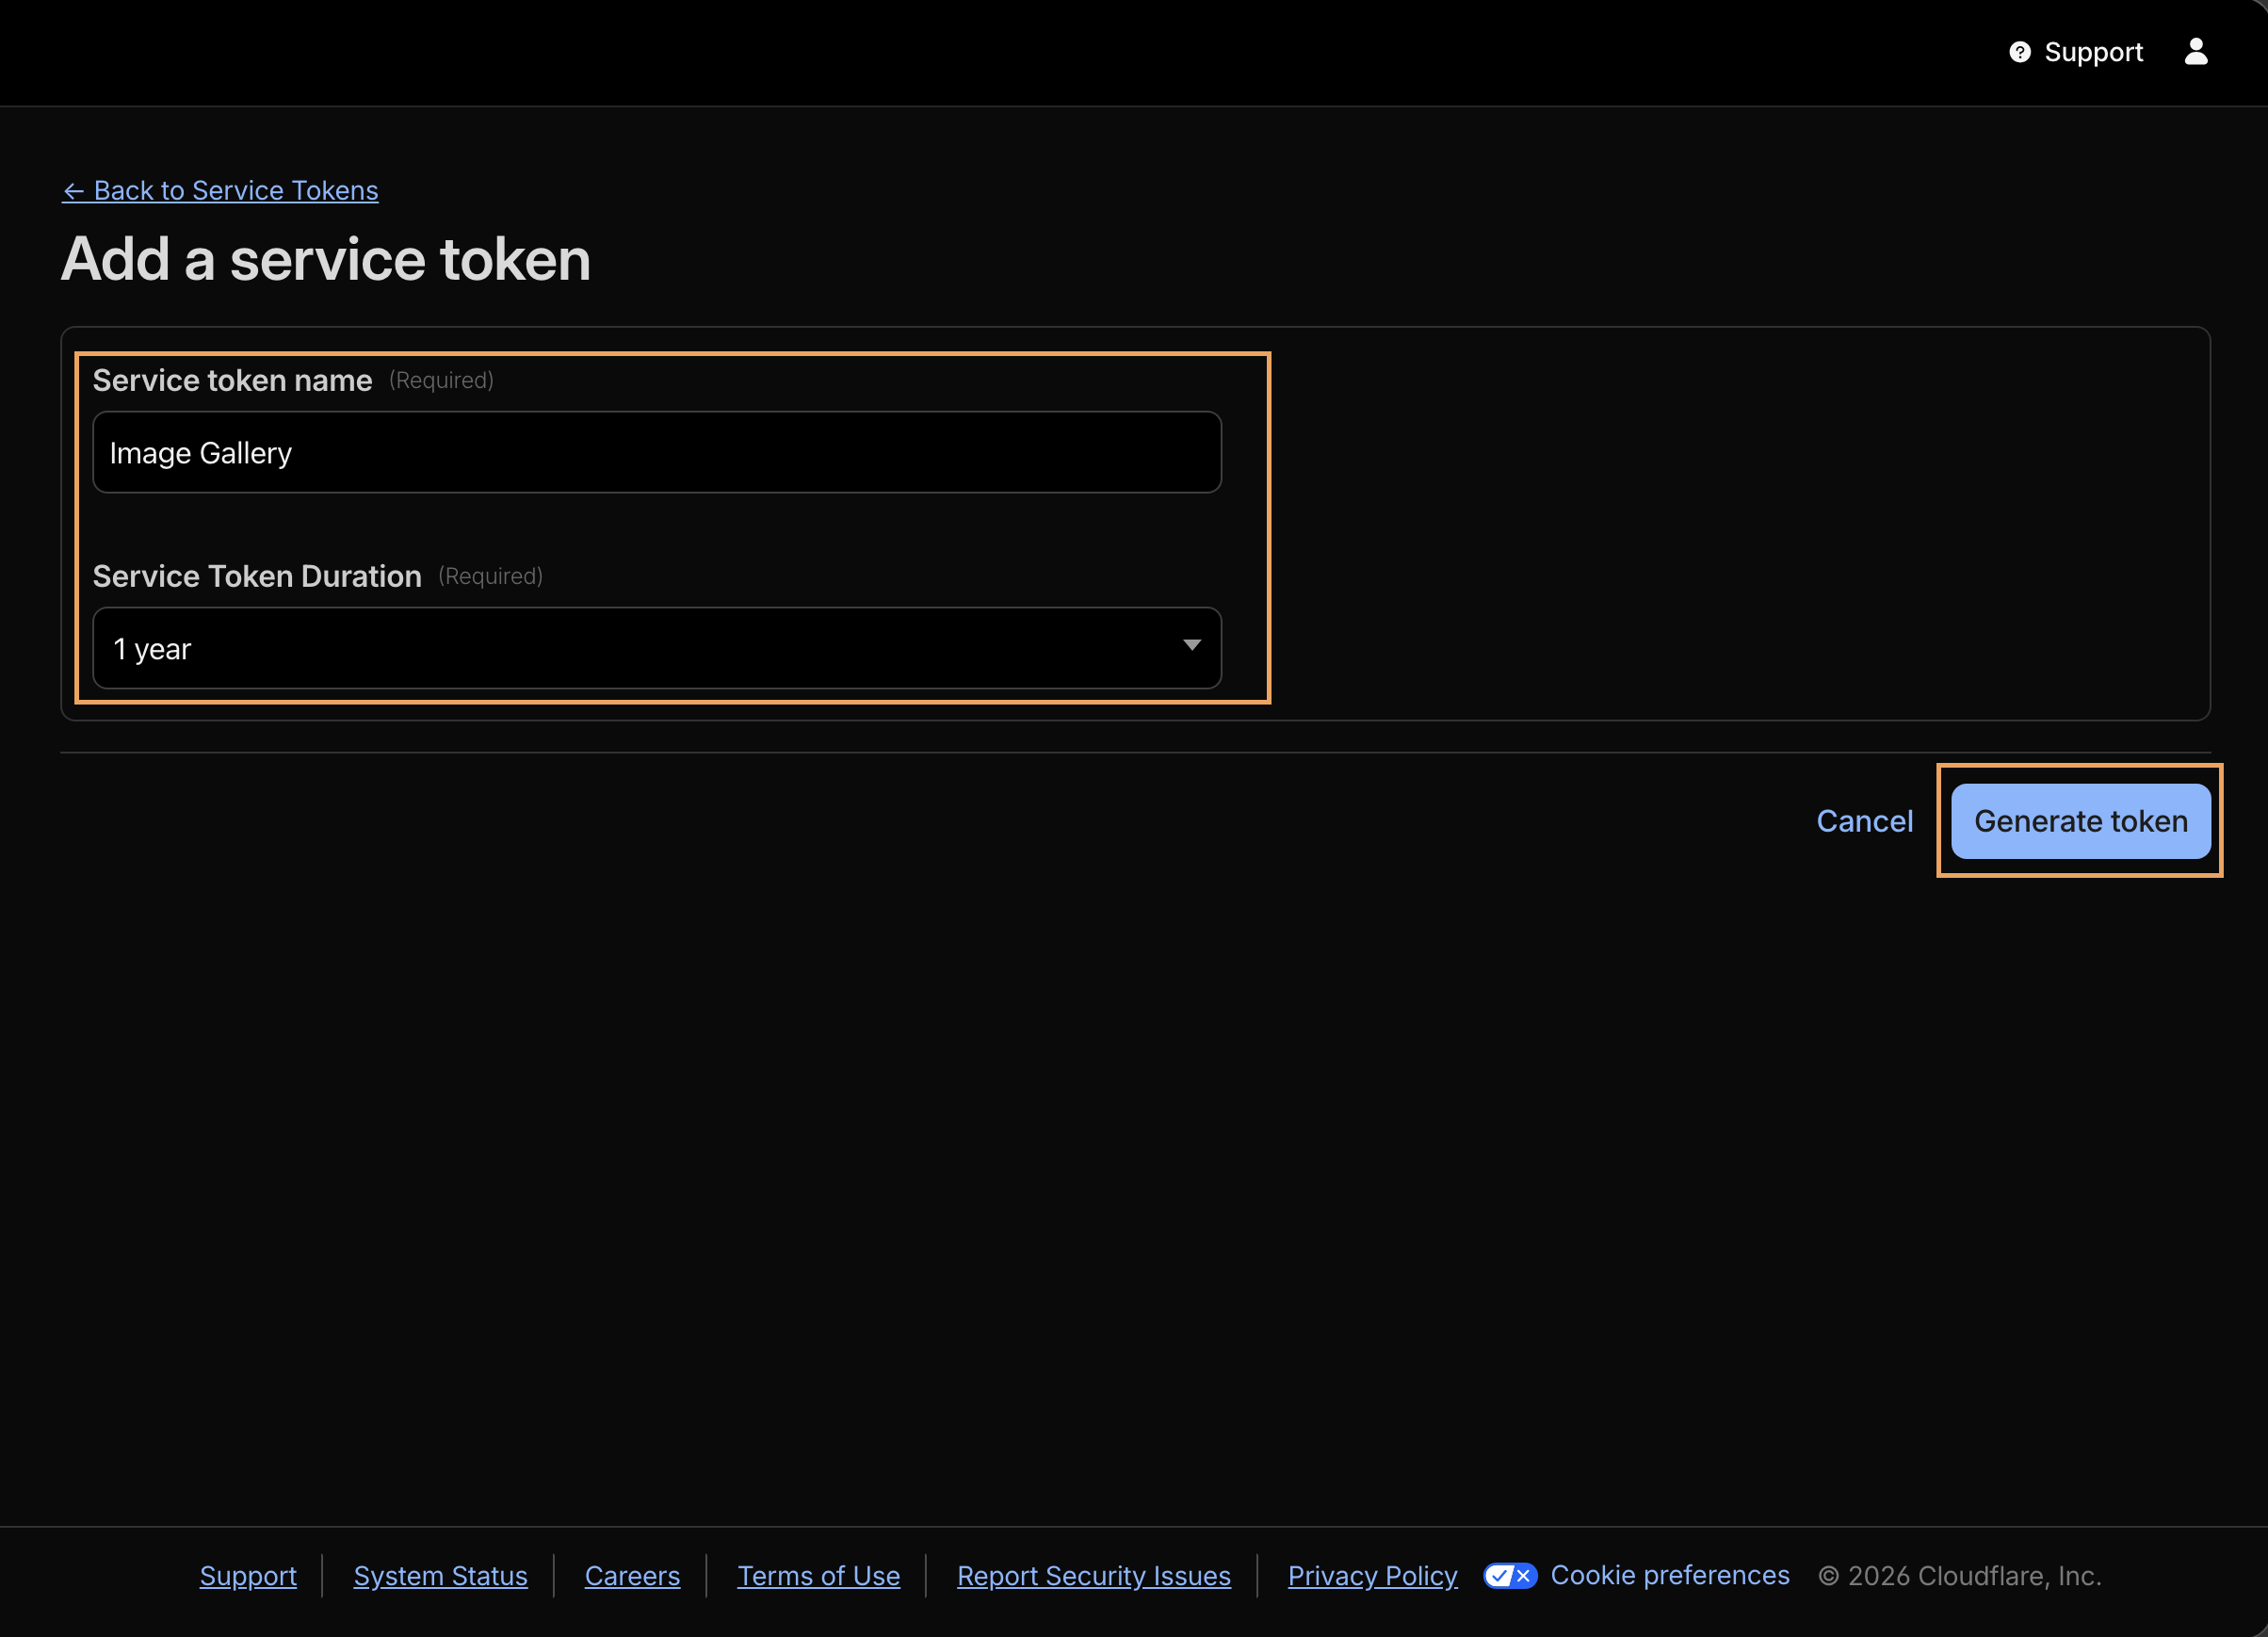
\includegraphics[width=0.5\textwidth]{media/token/token_2.png}
  \item Finally, save your \textbf{Client Id} and \textbf{Client Secret}\\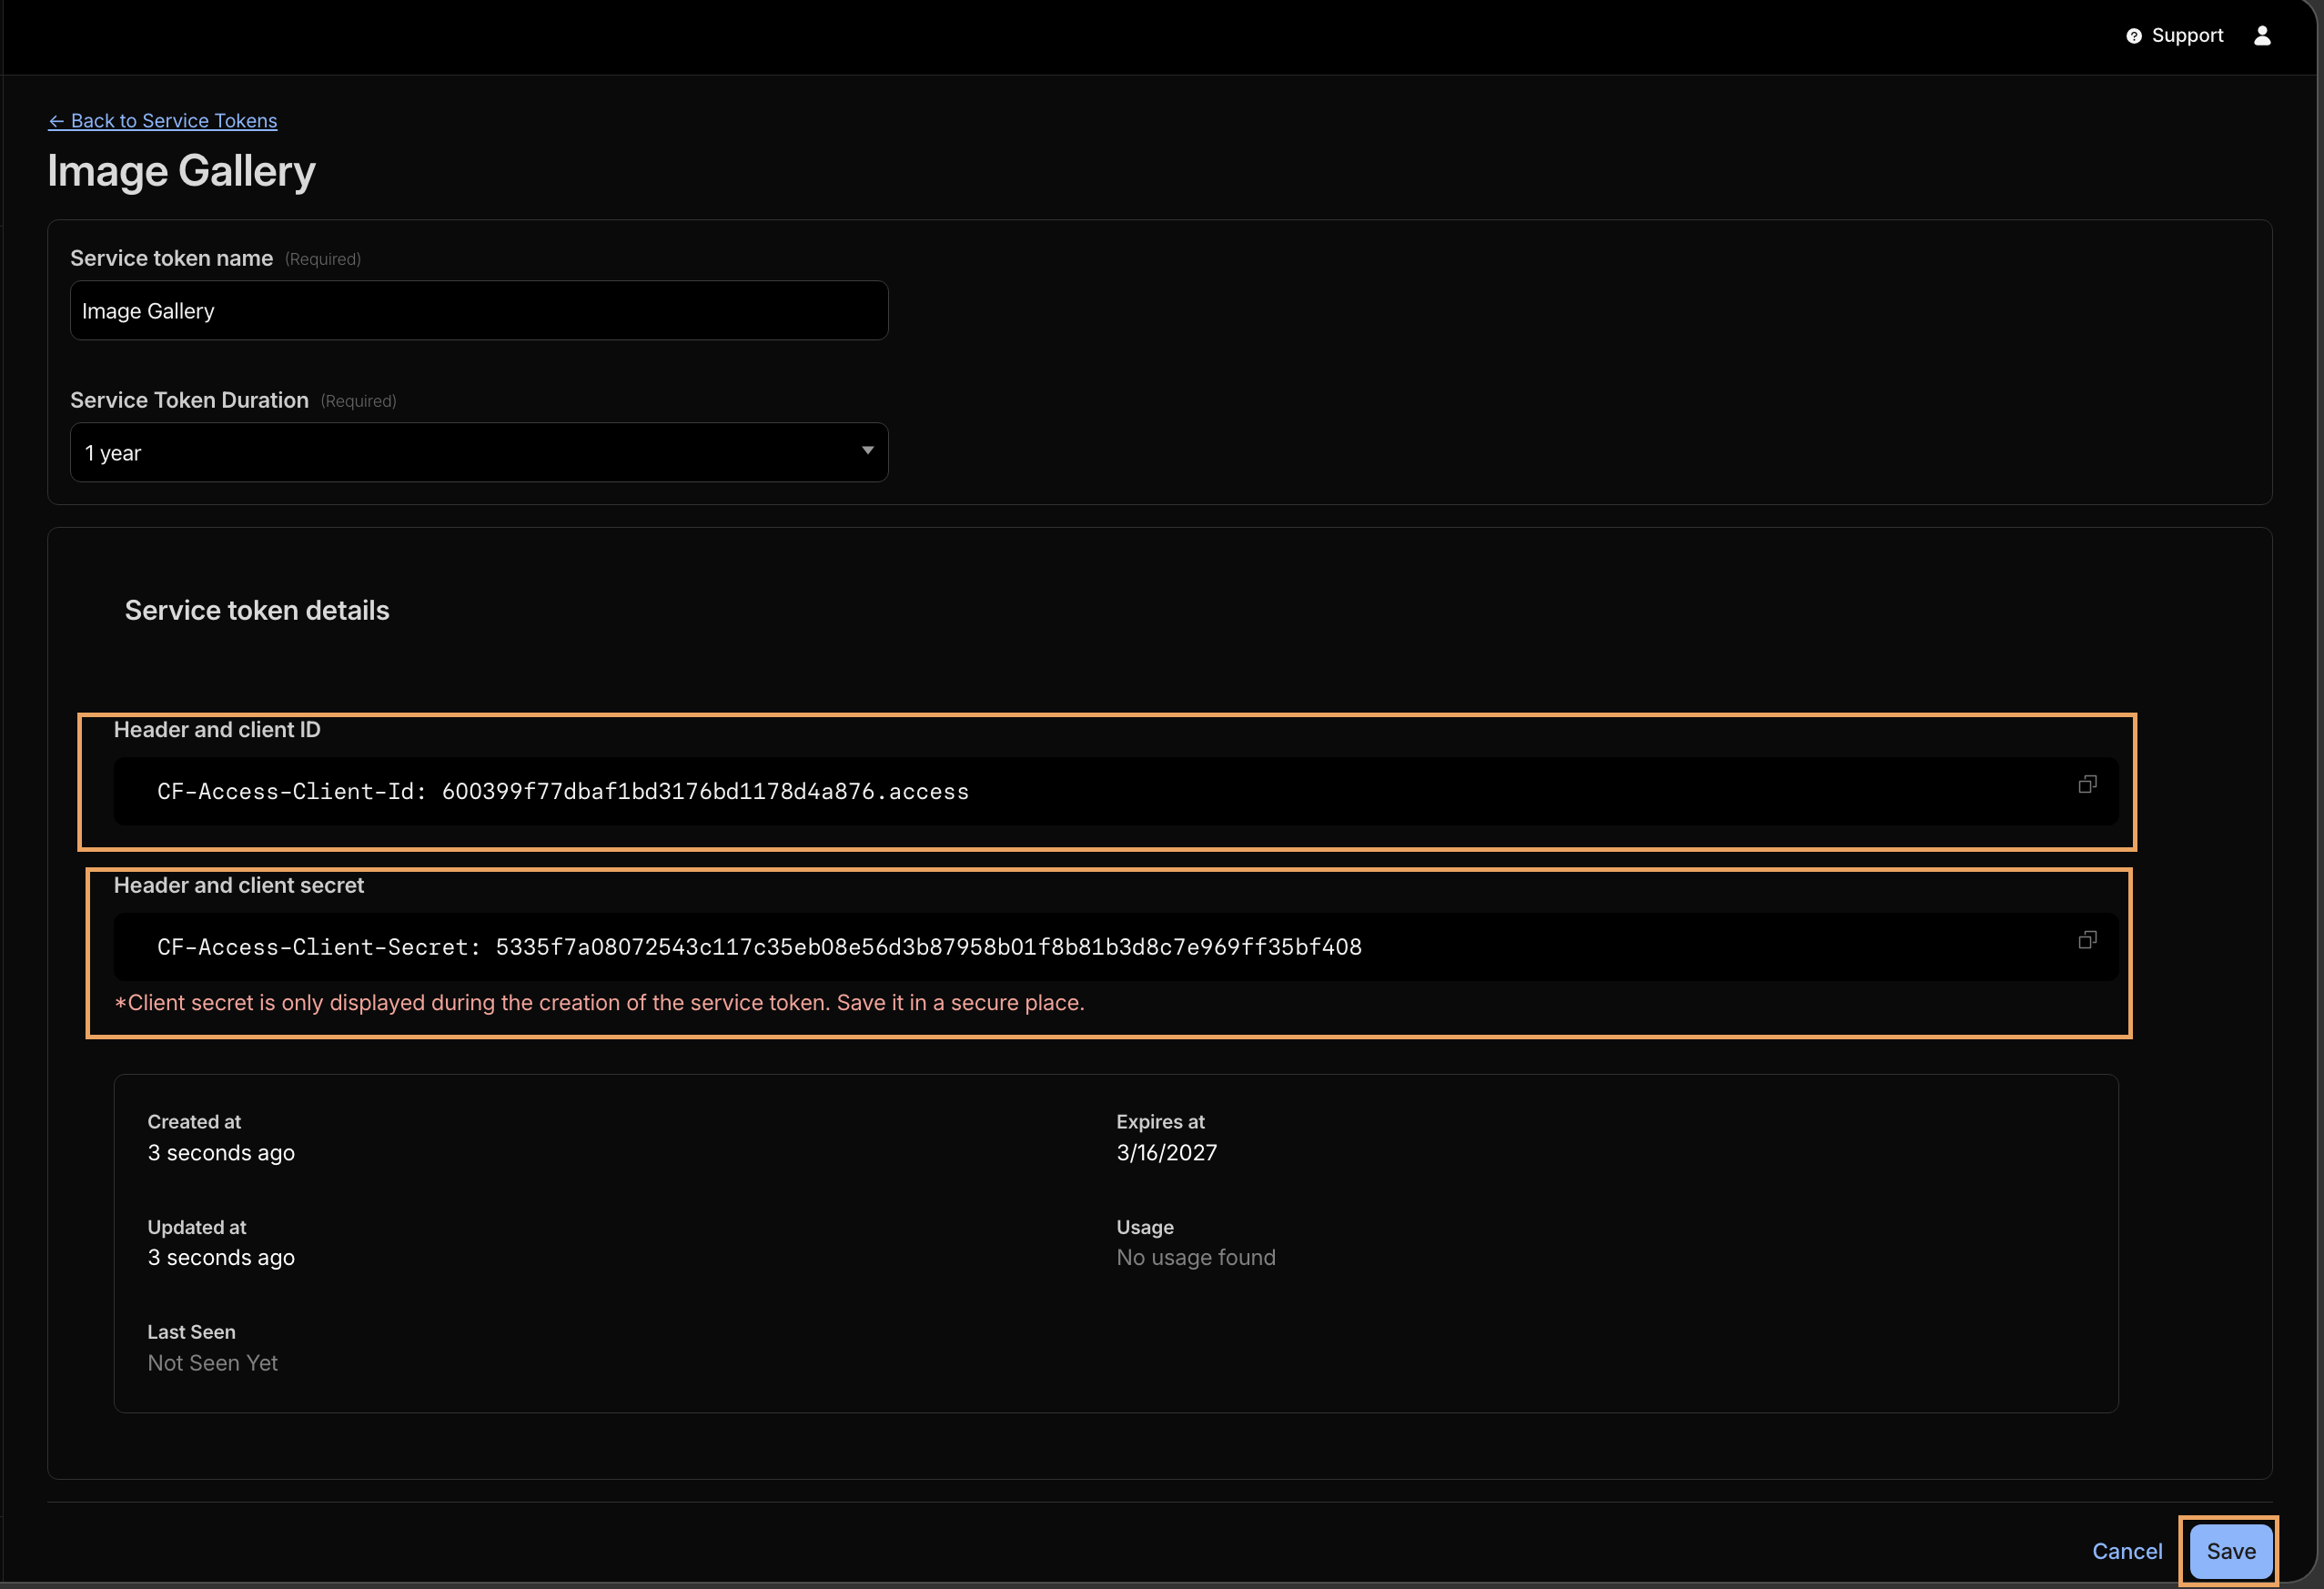
\includegraphics[width=0.5\textwidth]{media/token/token_3.png}
  \item Then, use Wrangler to put these values in the \textbf{Secret Store}\\\texttt{npx wrangler secret put CF-Access-Client-Secret}\\\texttt{npx wrangler secret put CF-Access-Client-Id}
\end{enumerate}

\subsection{Security Policy Creation}
\begin{enumerate}[leftmargin=*]
  \item Login to \href{https://dash.cloudflare.com}{Cloudflare Dashboard}
  \item Go to \textbf{Zero Trust}, \textbf{Access Controls} and then \textbf{Policies}
  \item Then, \textbf{Add a policy}\\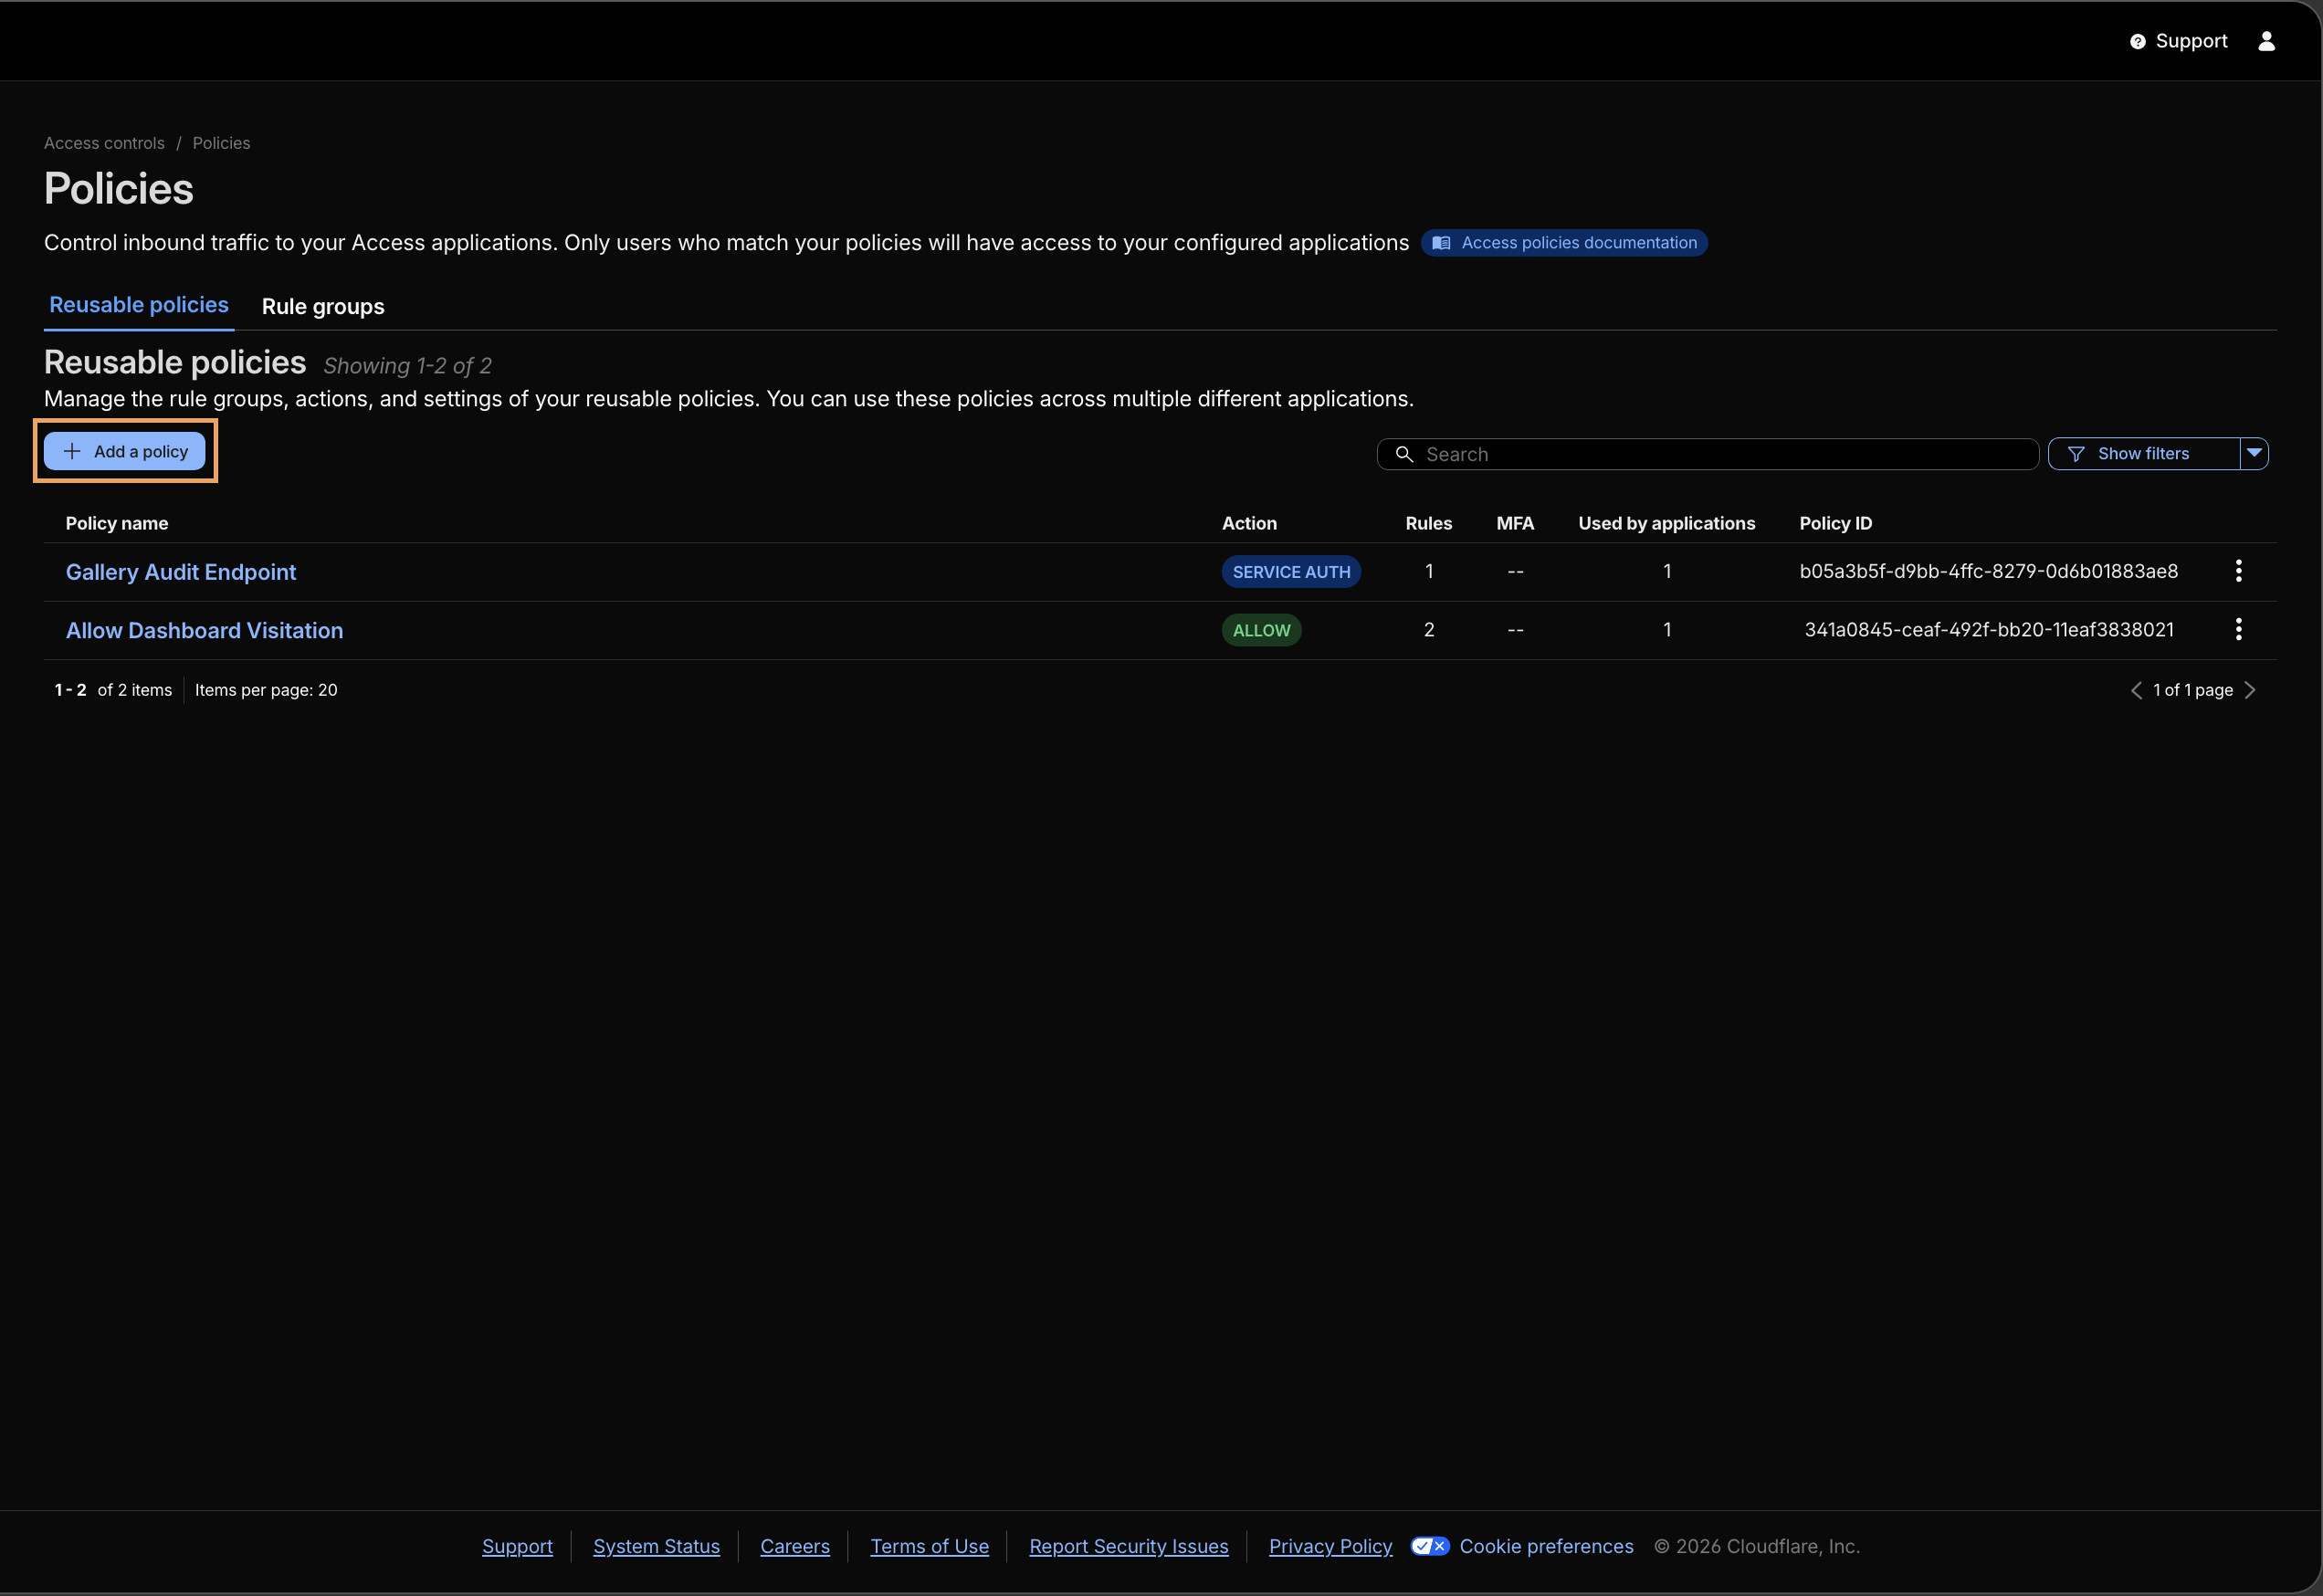
\includegraphics[width=0.5\textwidth]{media/pol/pol_1.png}
  \item Set its action as \textbf{Service Auth}, add a policy name, and its session duration\\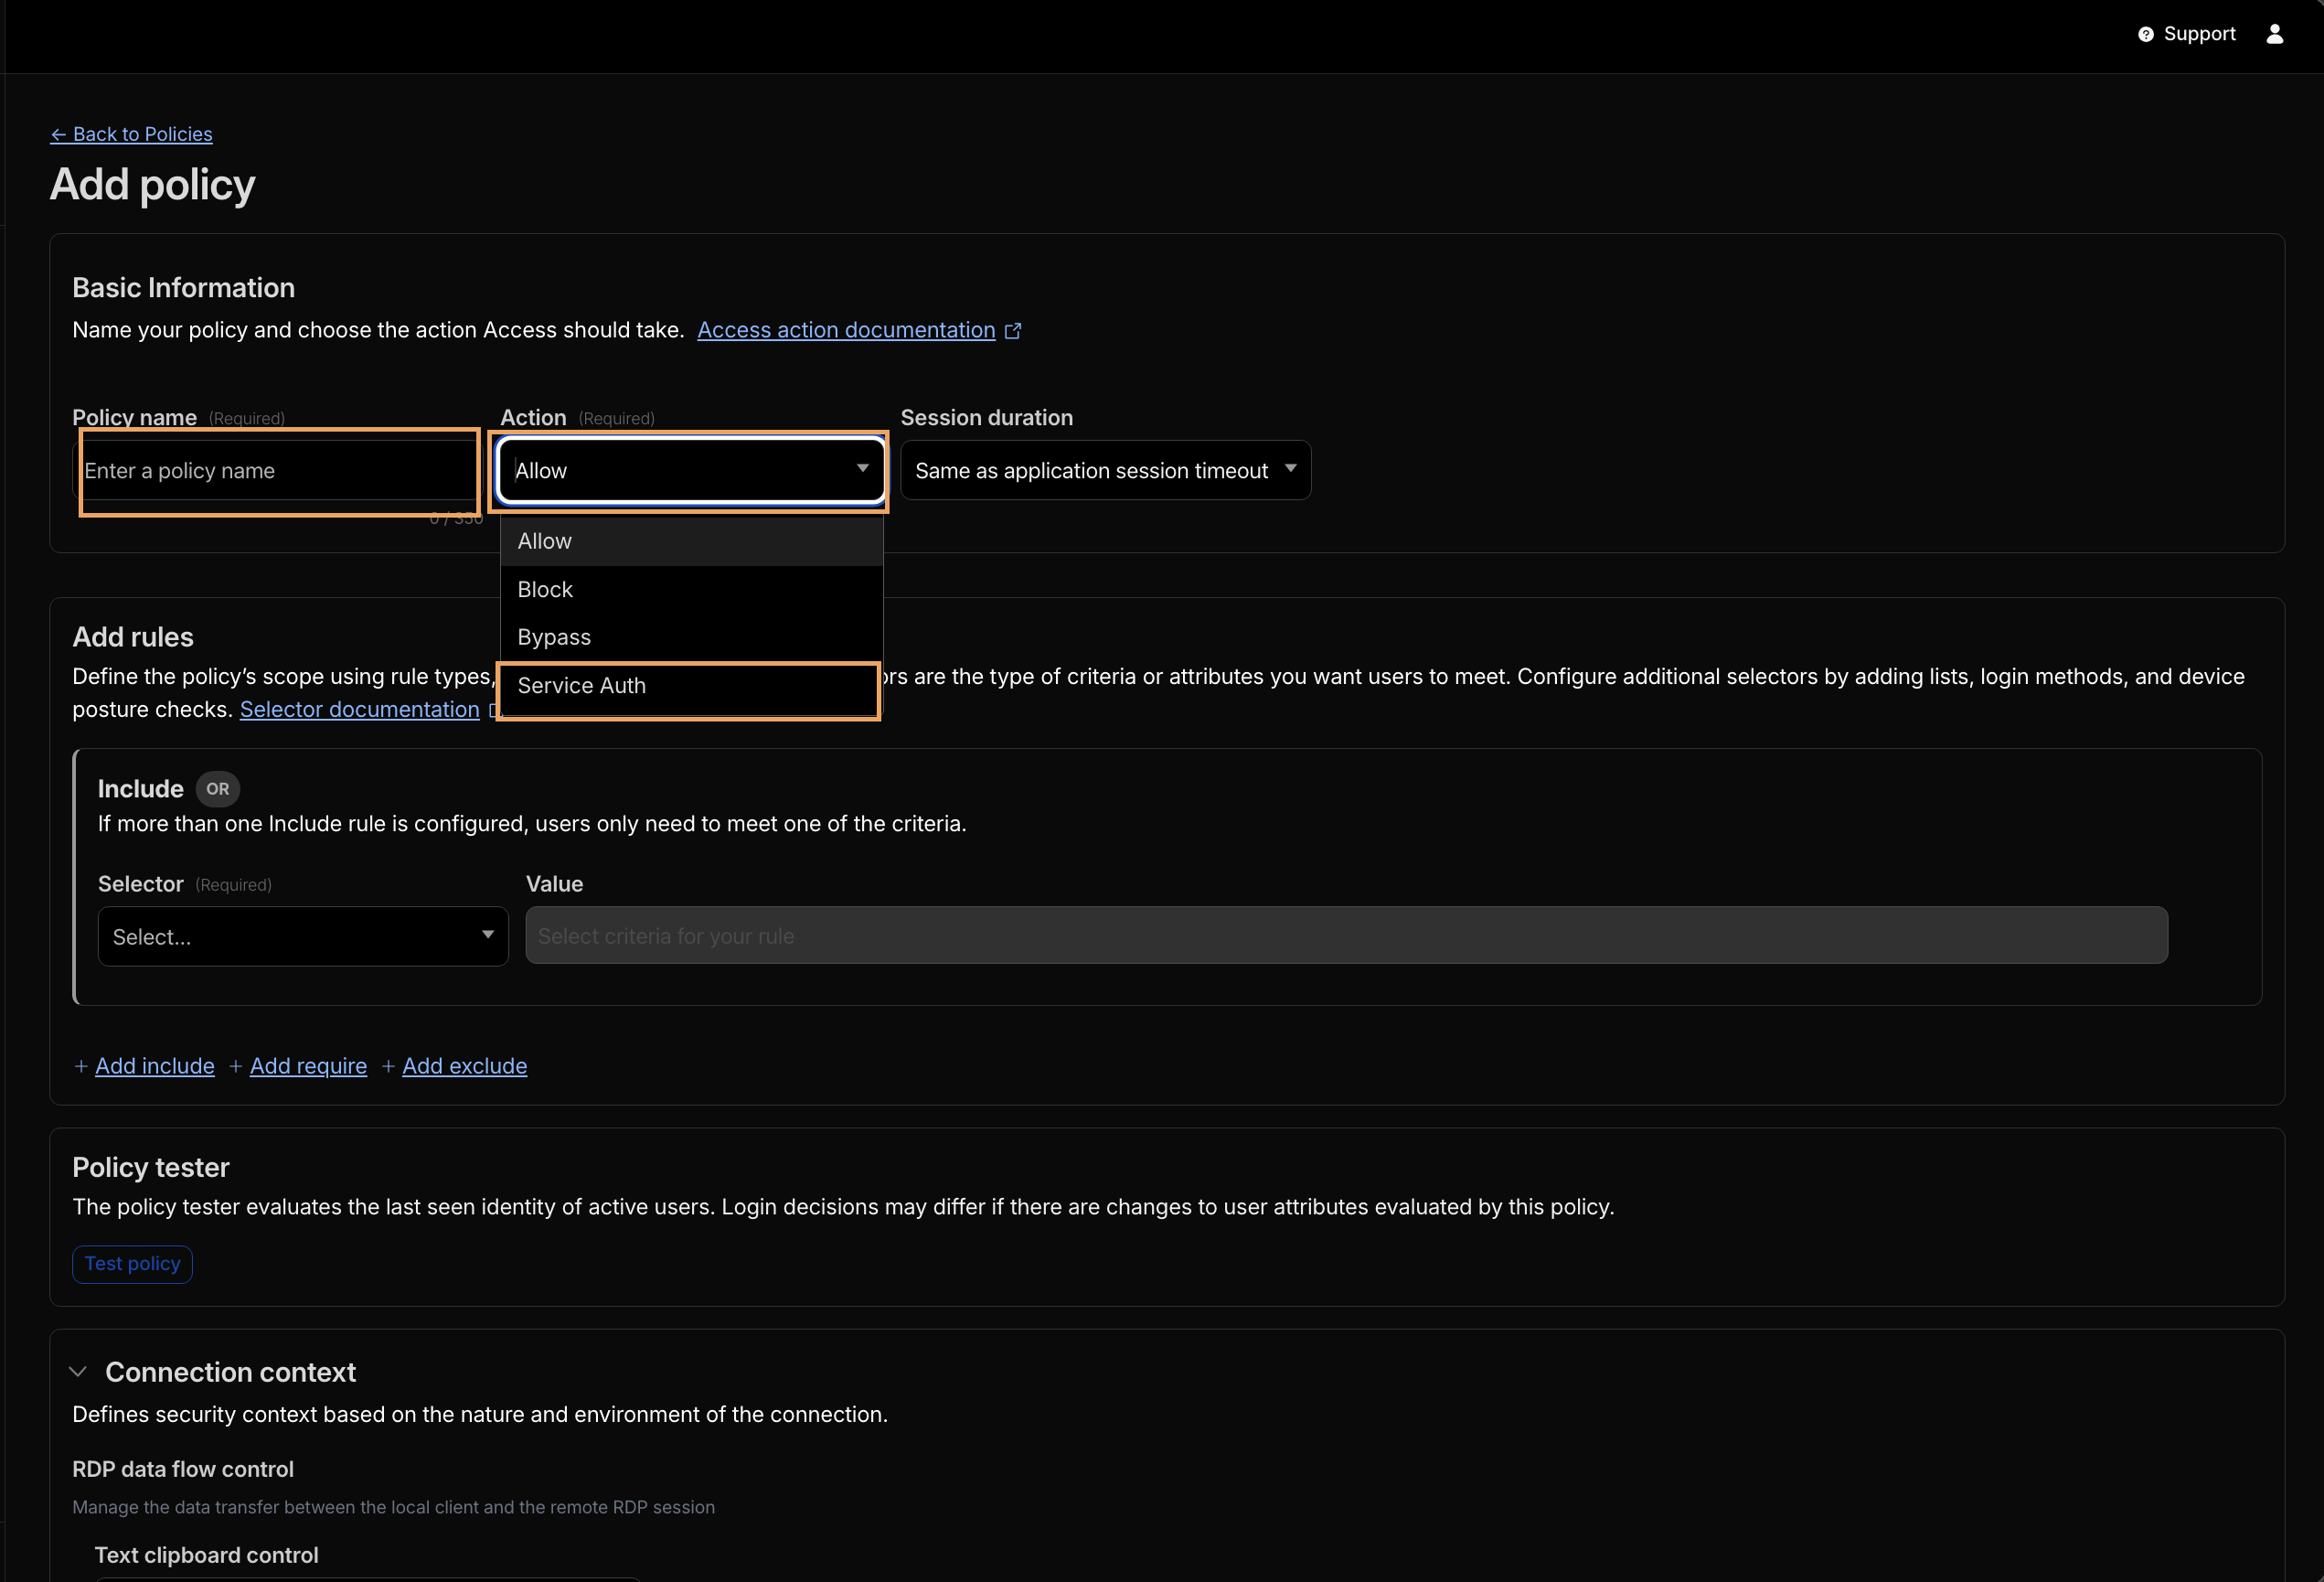
\includegraphics[width=0.5\textwidth]{media/pol/pol_2.png}
  \item Then, add an \textbf{include rule} and select \textbf{Service Token}\\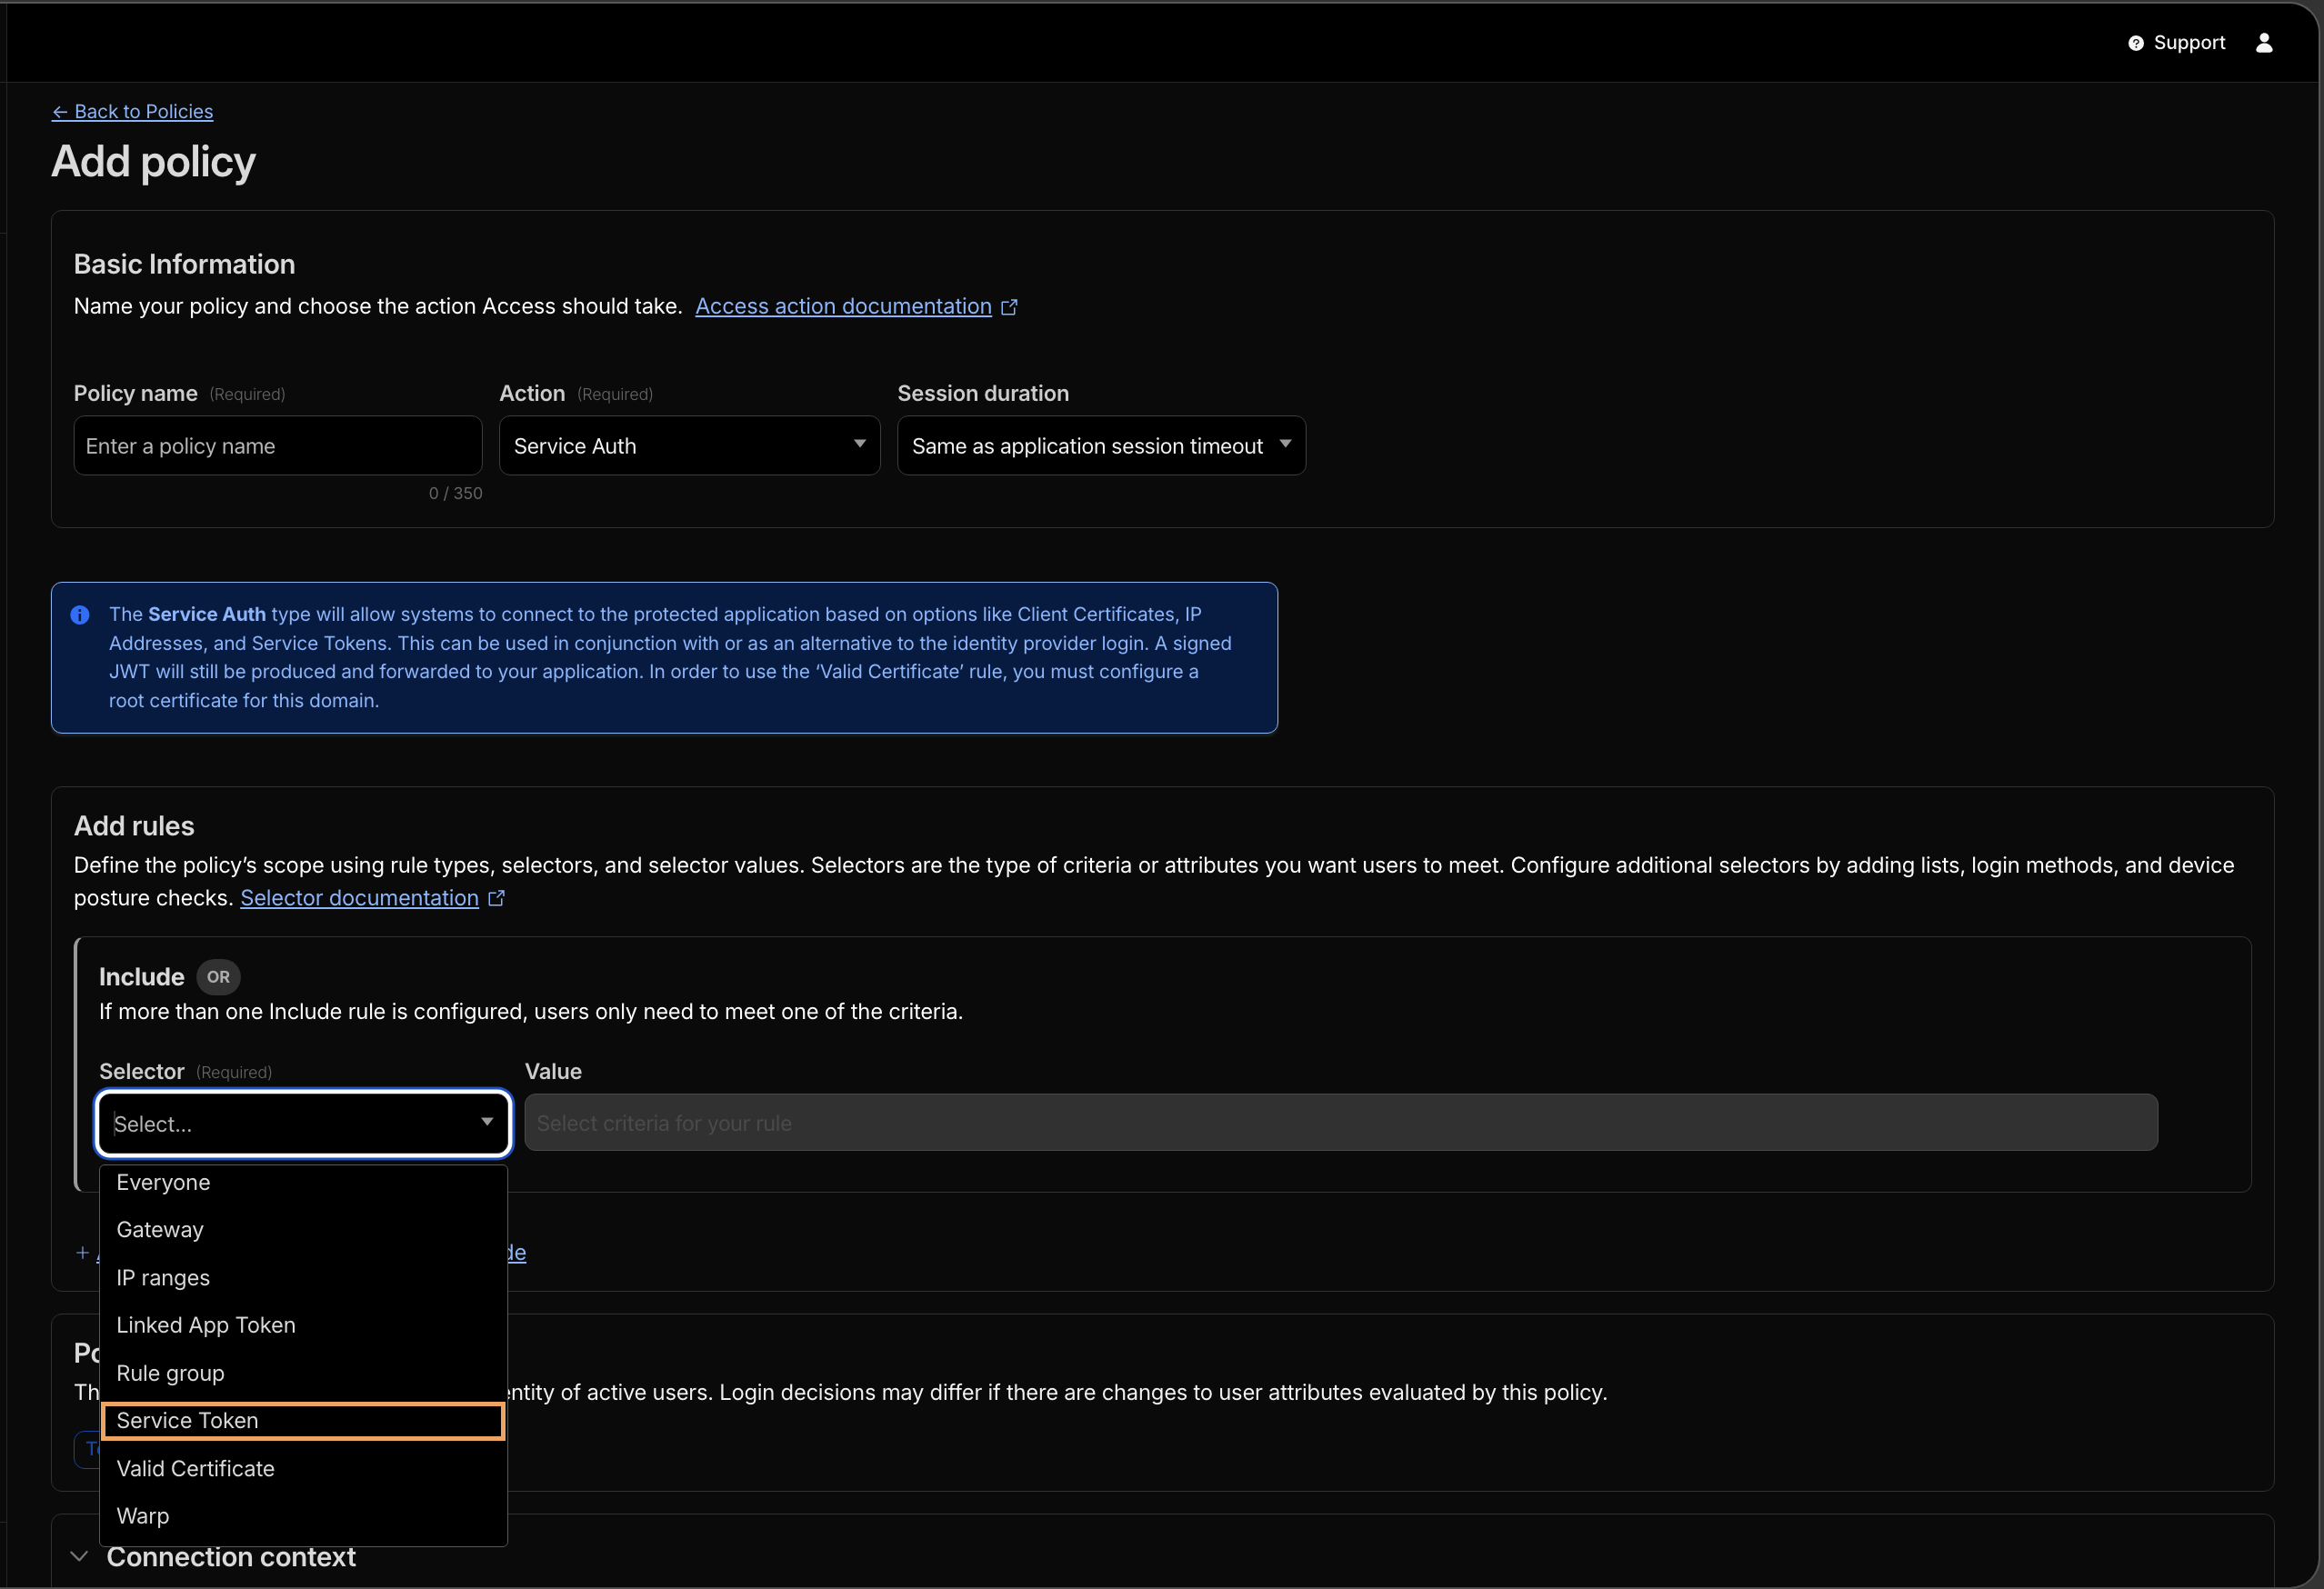
\includegraphics[width=0.5\textwidth]{media/pol/pol_3.png}
  \item Use the previously created token\\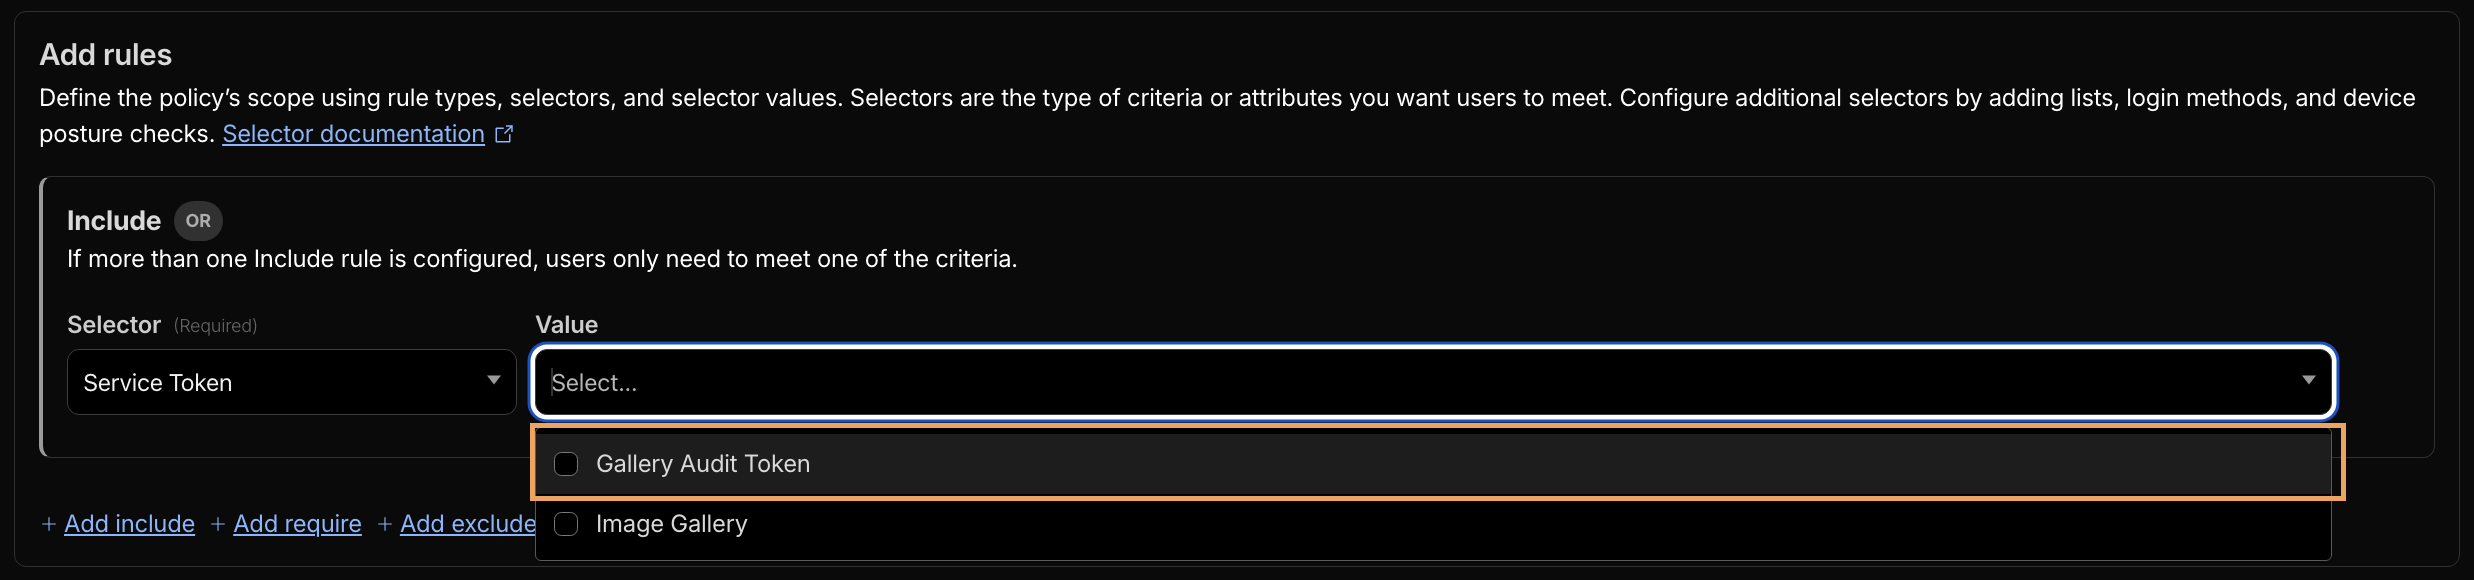
\includegraphics[width=0.5\textwidth]{media/pol/pol_4.png}
\end{enumerate}

\subsection{Access Policy Creation}
\begin{enumerate}[leftmargin=*]
  \item Login to \href{https://dash.cloudflare.com}{Cloudflare Dashboard}
  \item Go to \textbf{Zero Trust}, \textbf{Access Controls} and then \textbf{Applications}
  \item Click \textbf{Add Application}\\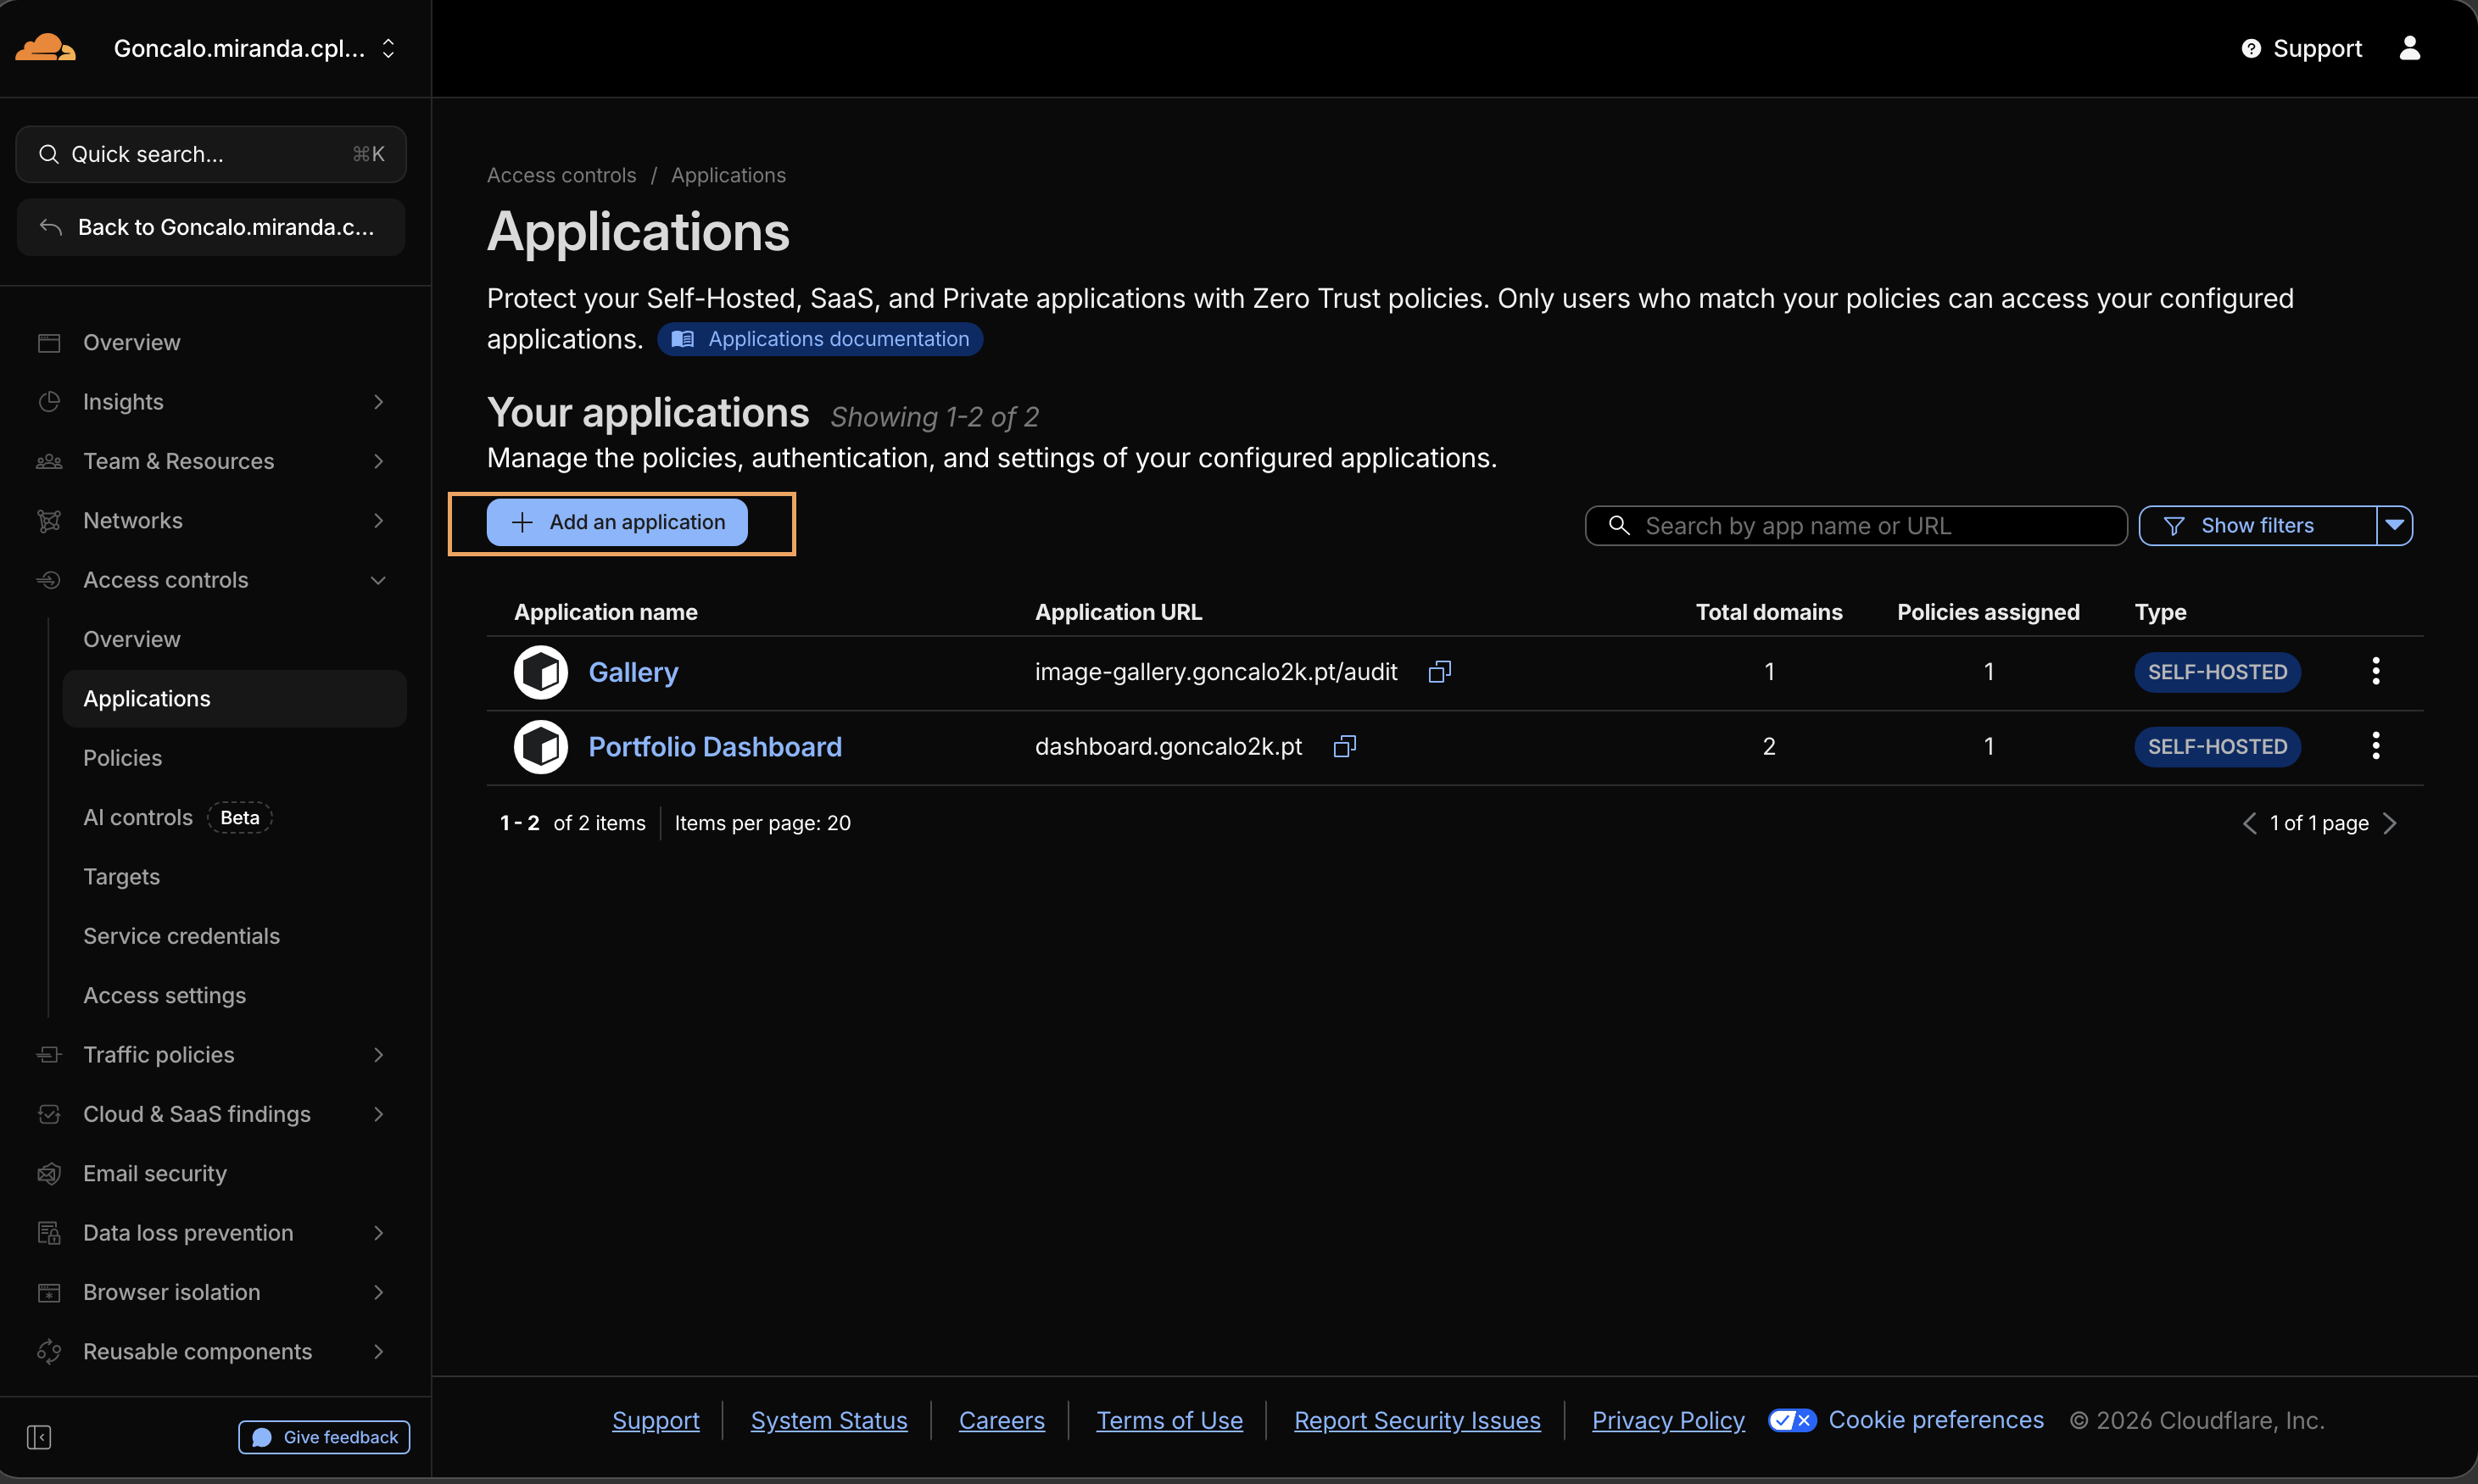
\includegraphics[width=0.5\textwidth]{media/zt/zt_1.png}
  \item Select \textbf{Self-hosted}\\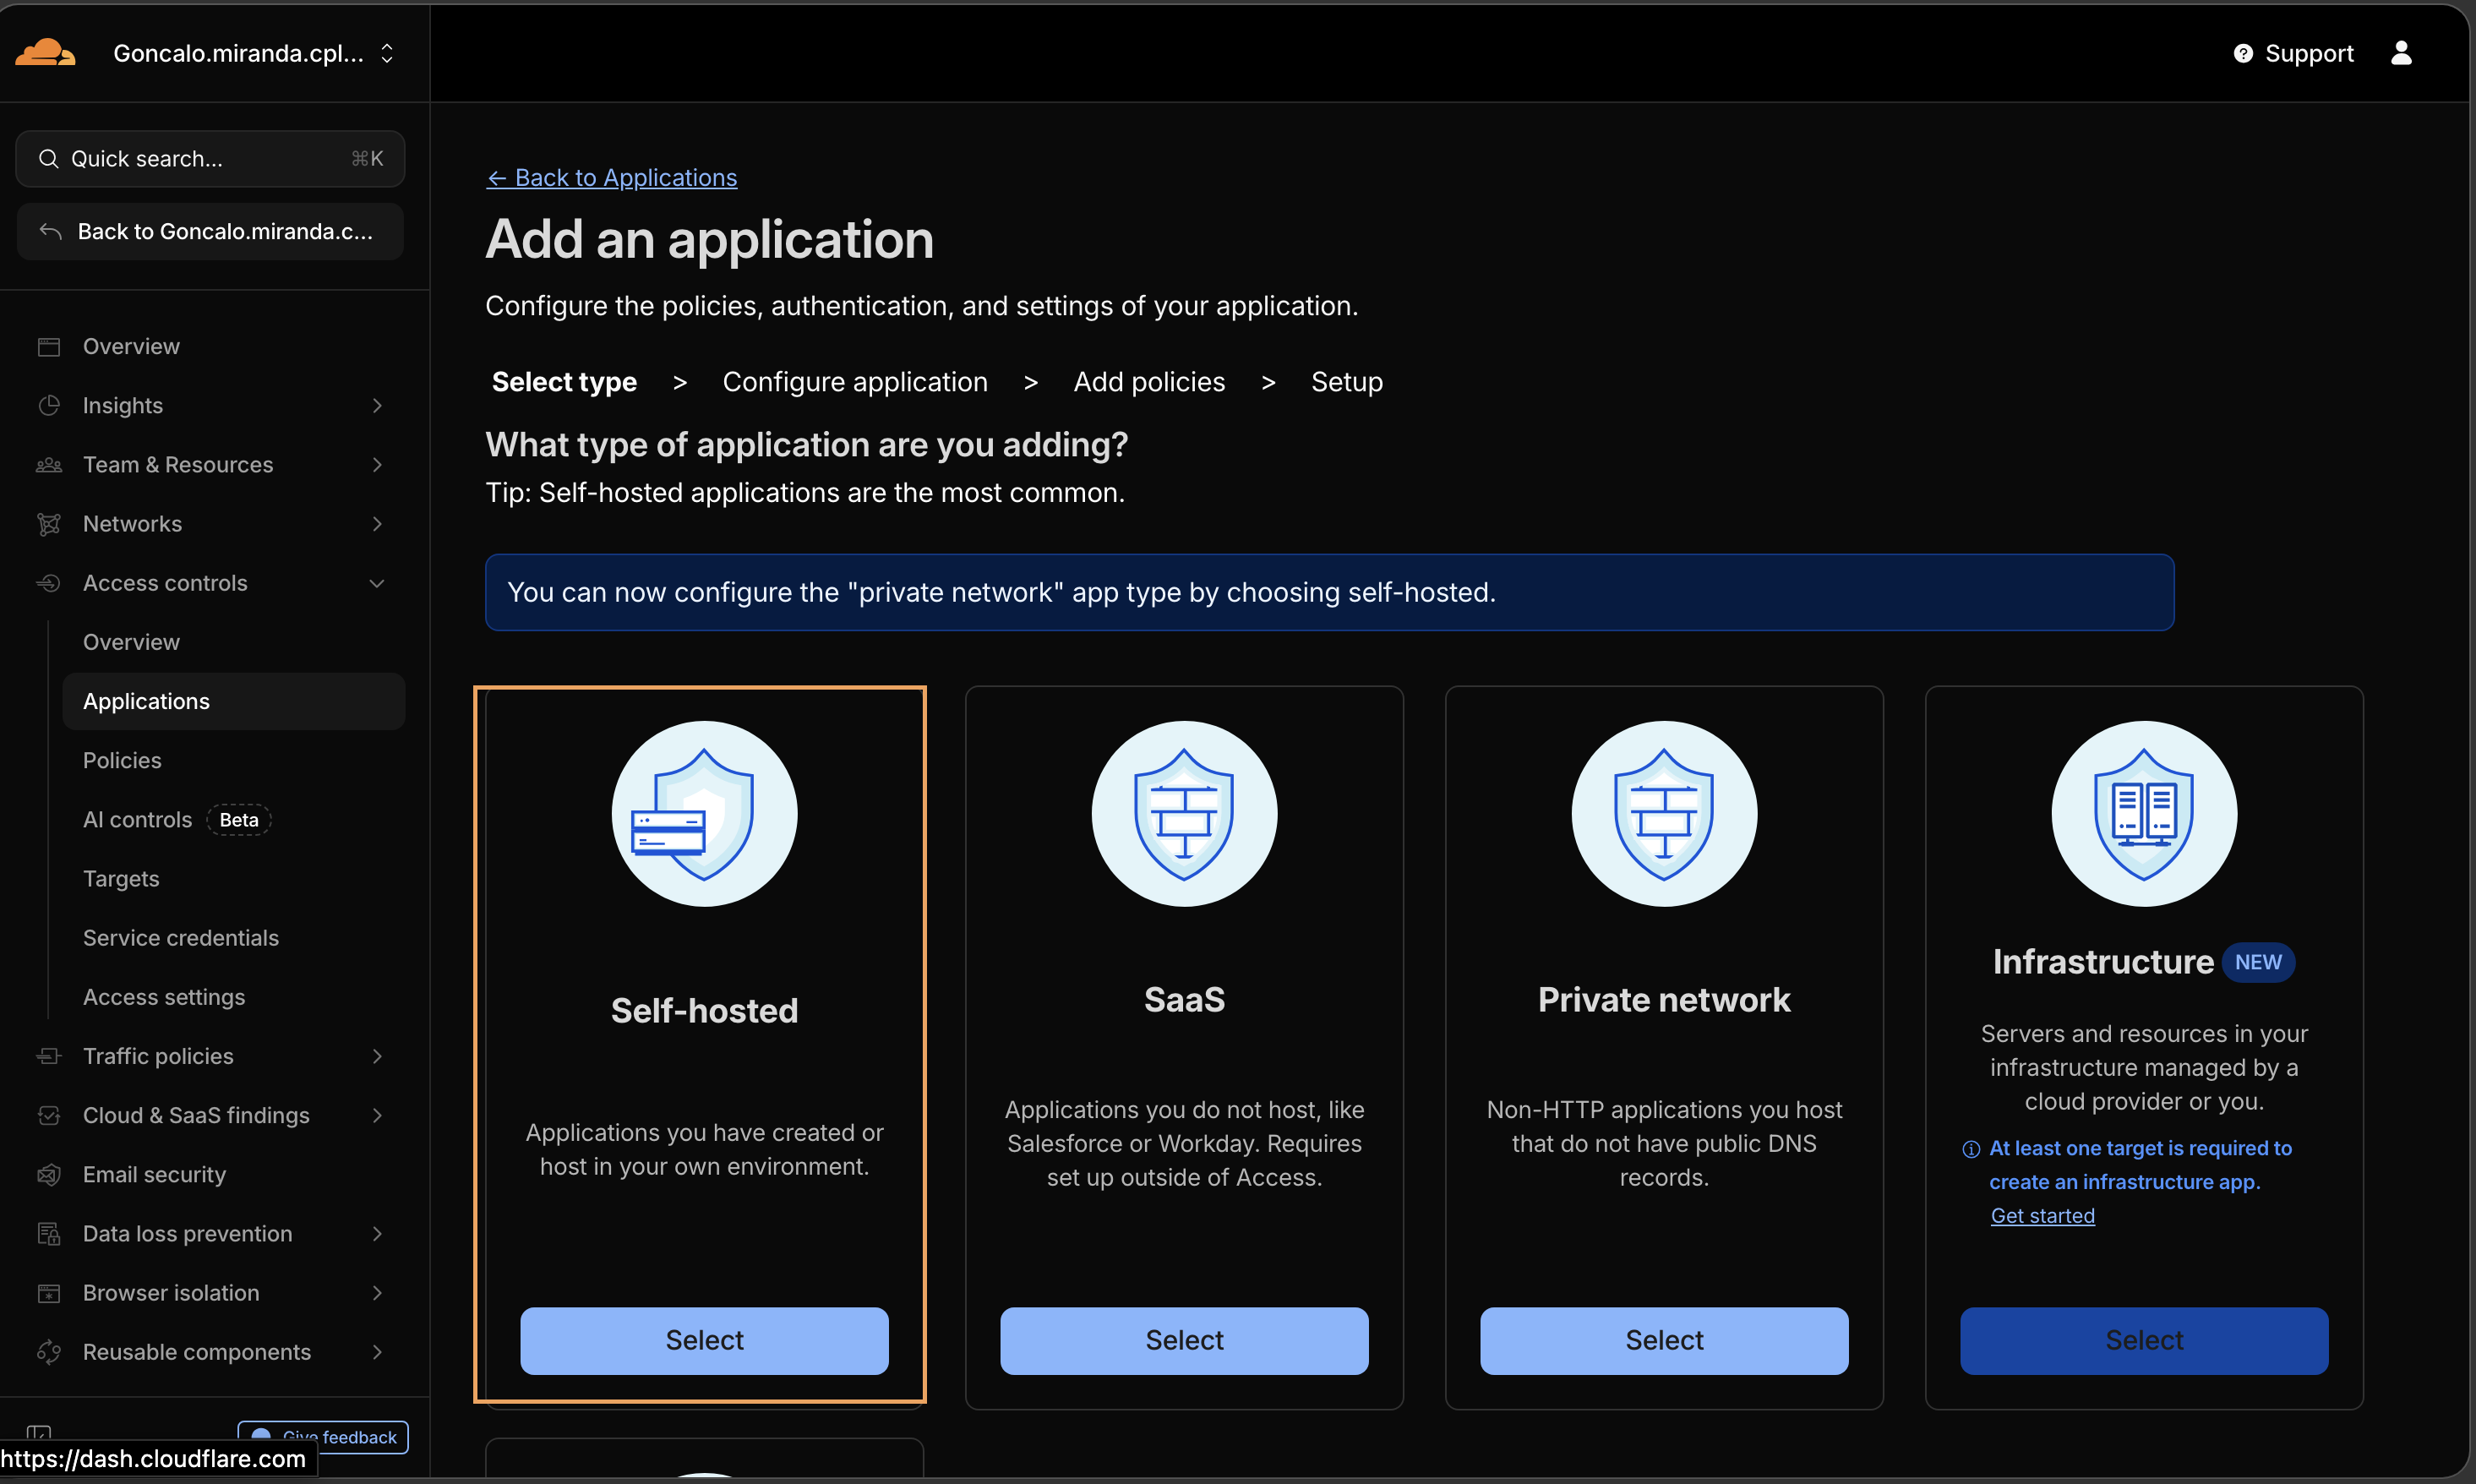
\includegraphics[width=0.5\textwidth]{media/zt/zt_2.png}
  \item Add the public hostname for the app you want to protect (in this case, image-gallery.goncalo2k.pt)\\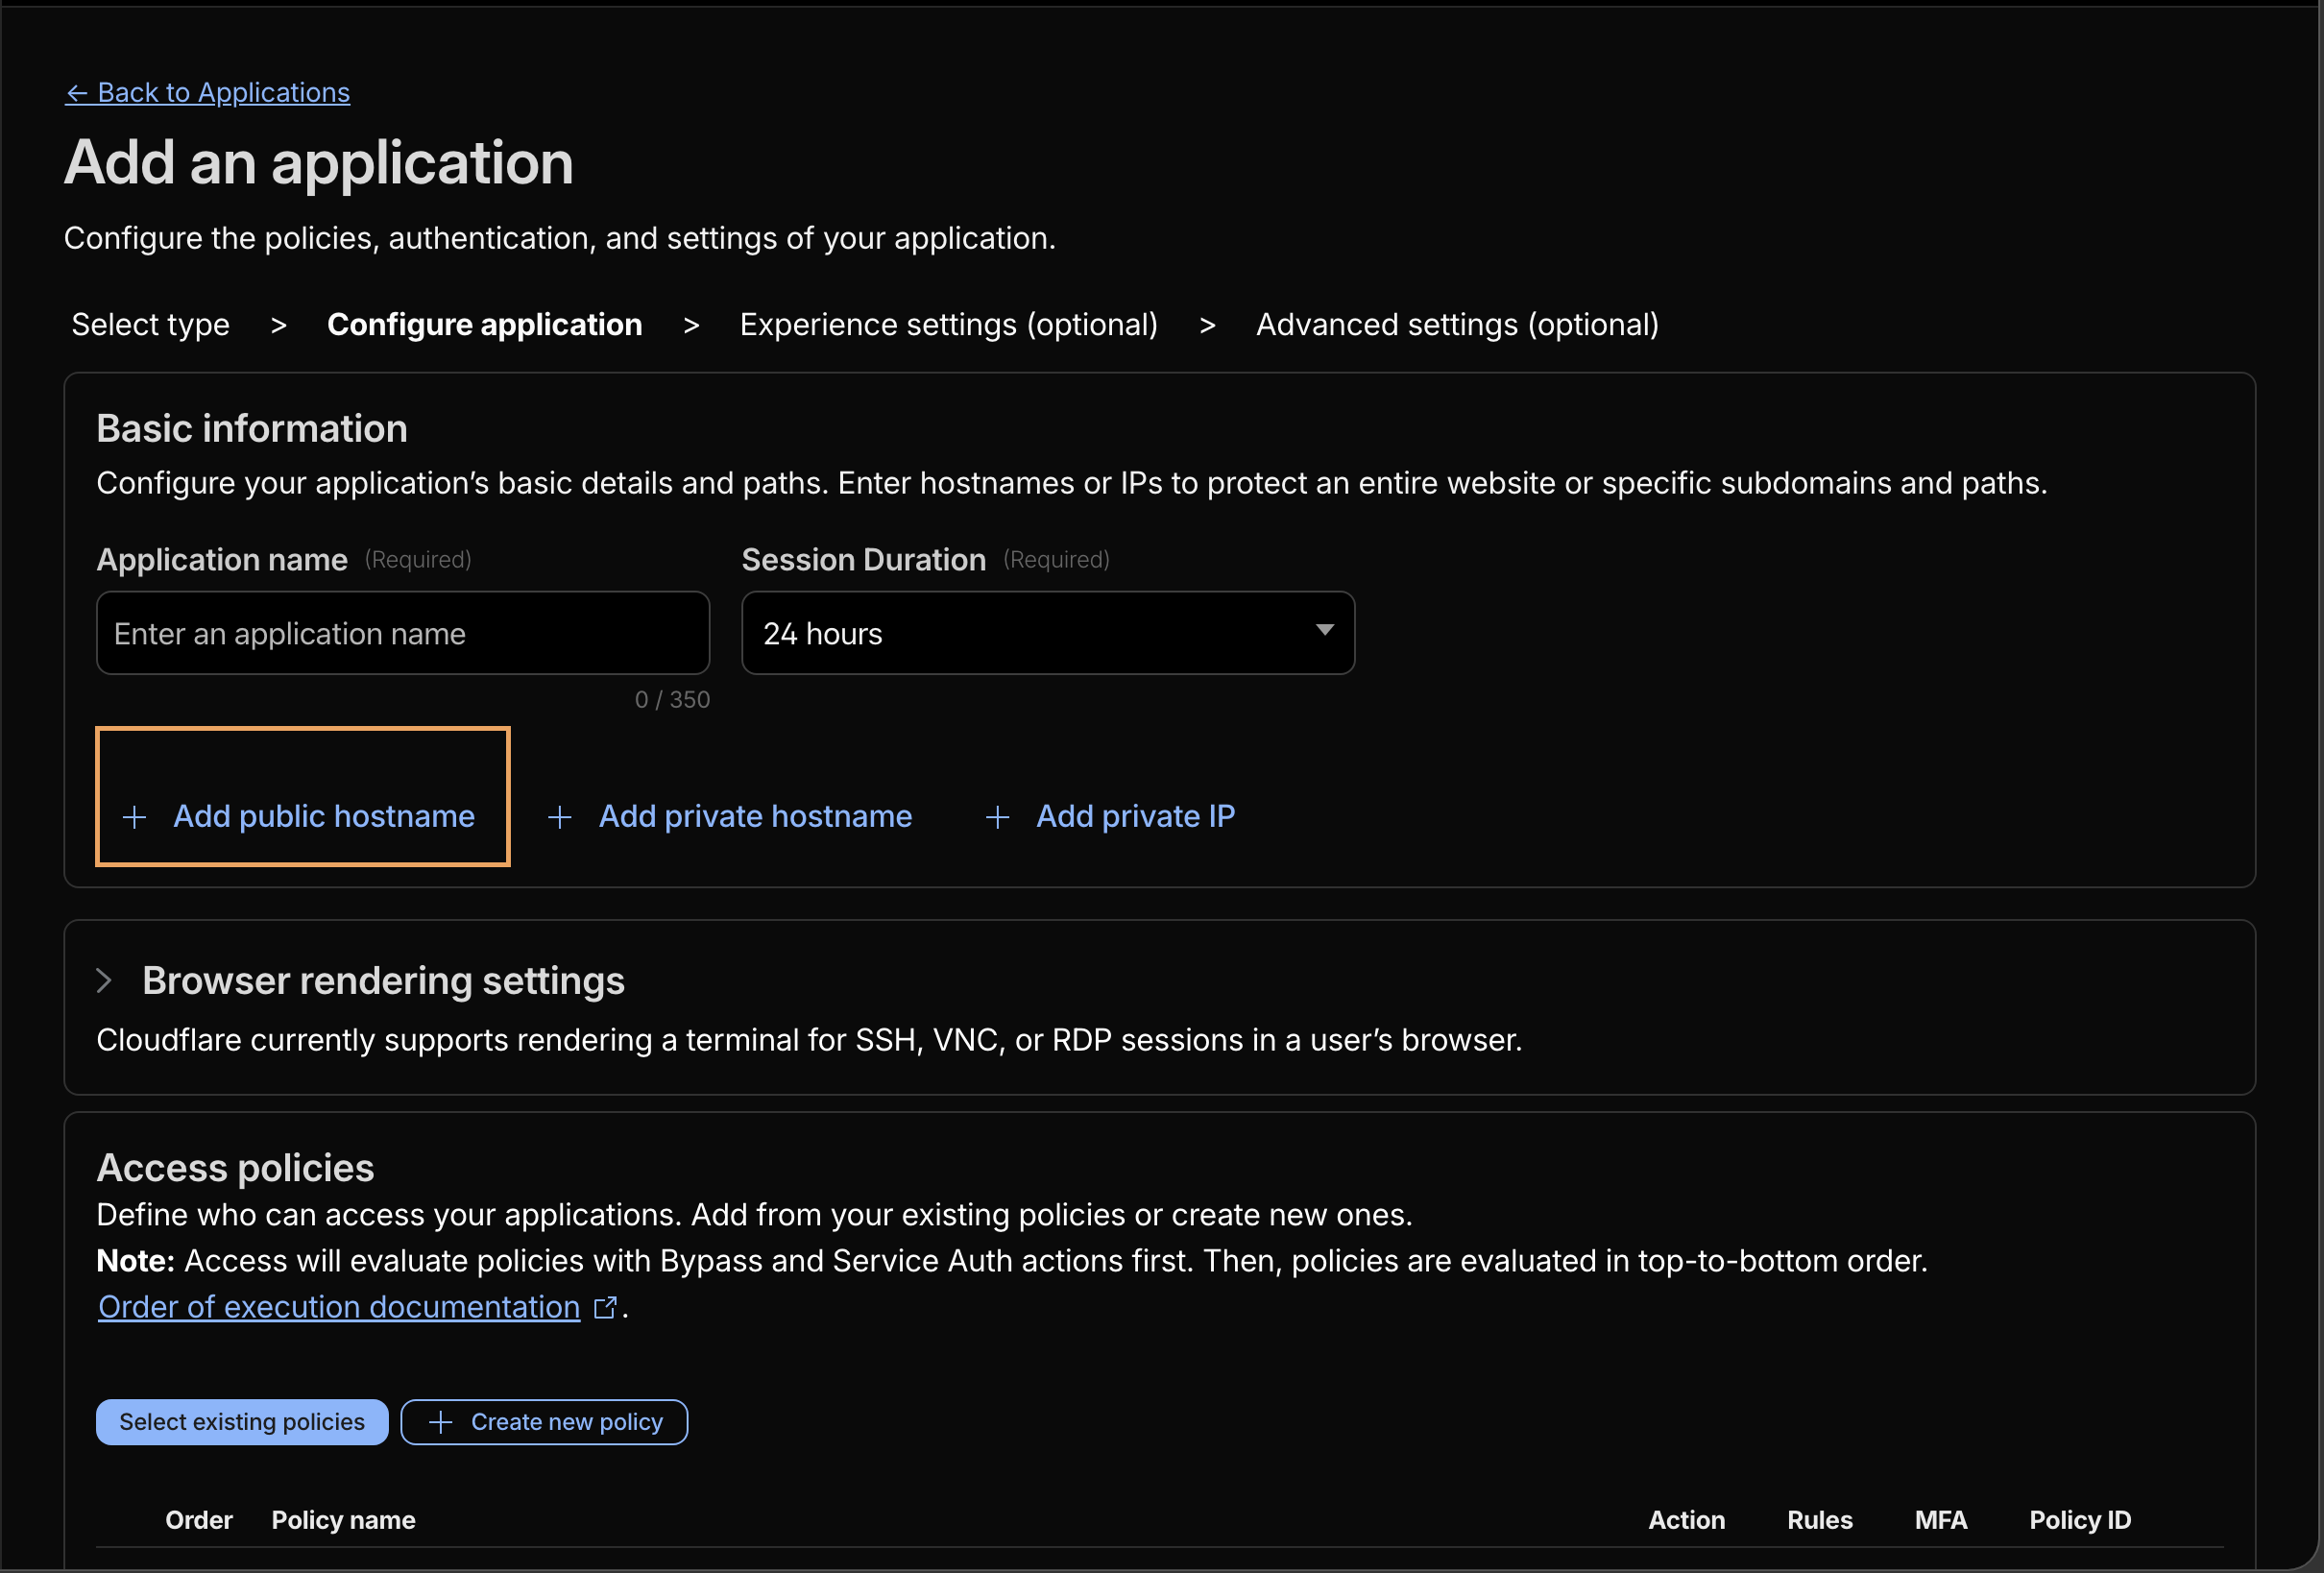
\includegraphics[width=0.5\textwidth]{media/zt/zt_3.png}
  \item Add Application name, session duration, and select the intended paths and subdomains if needed.\\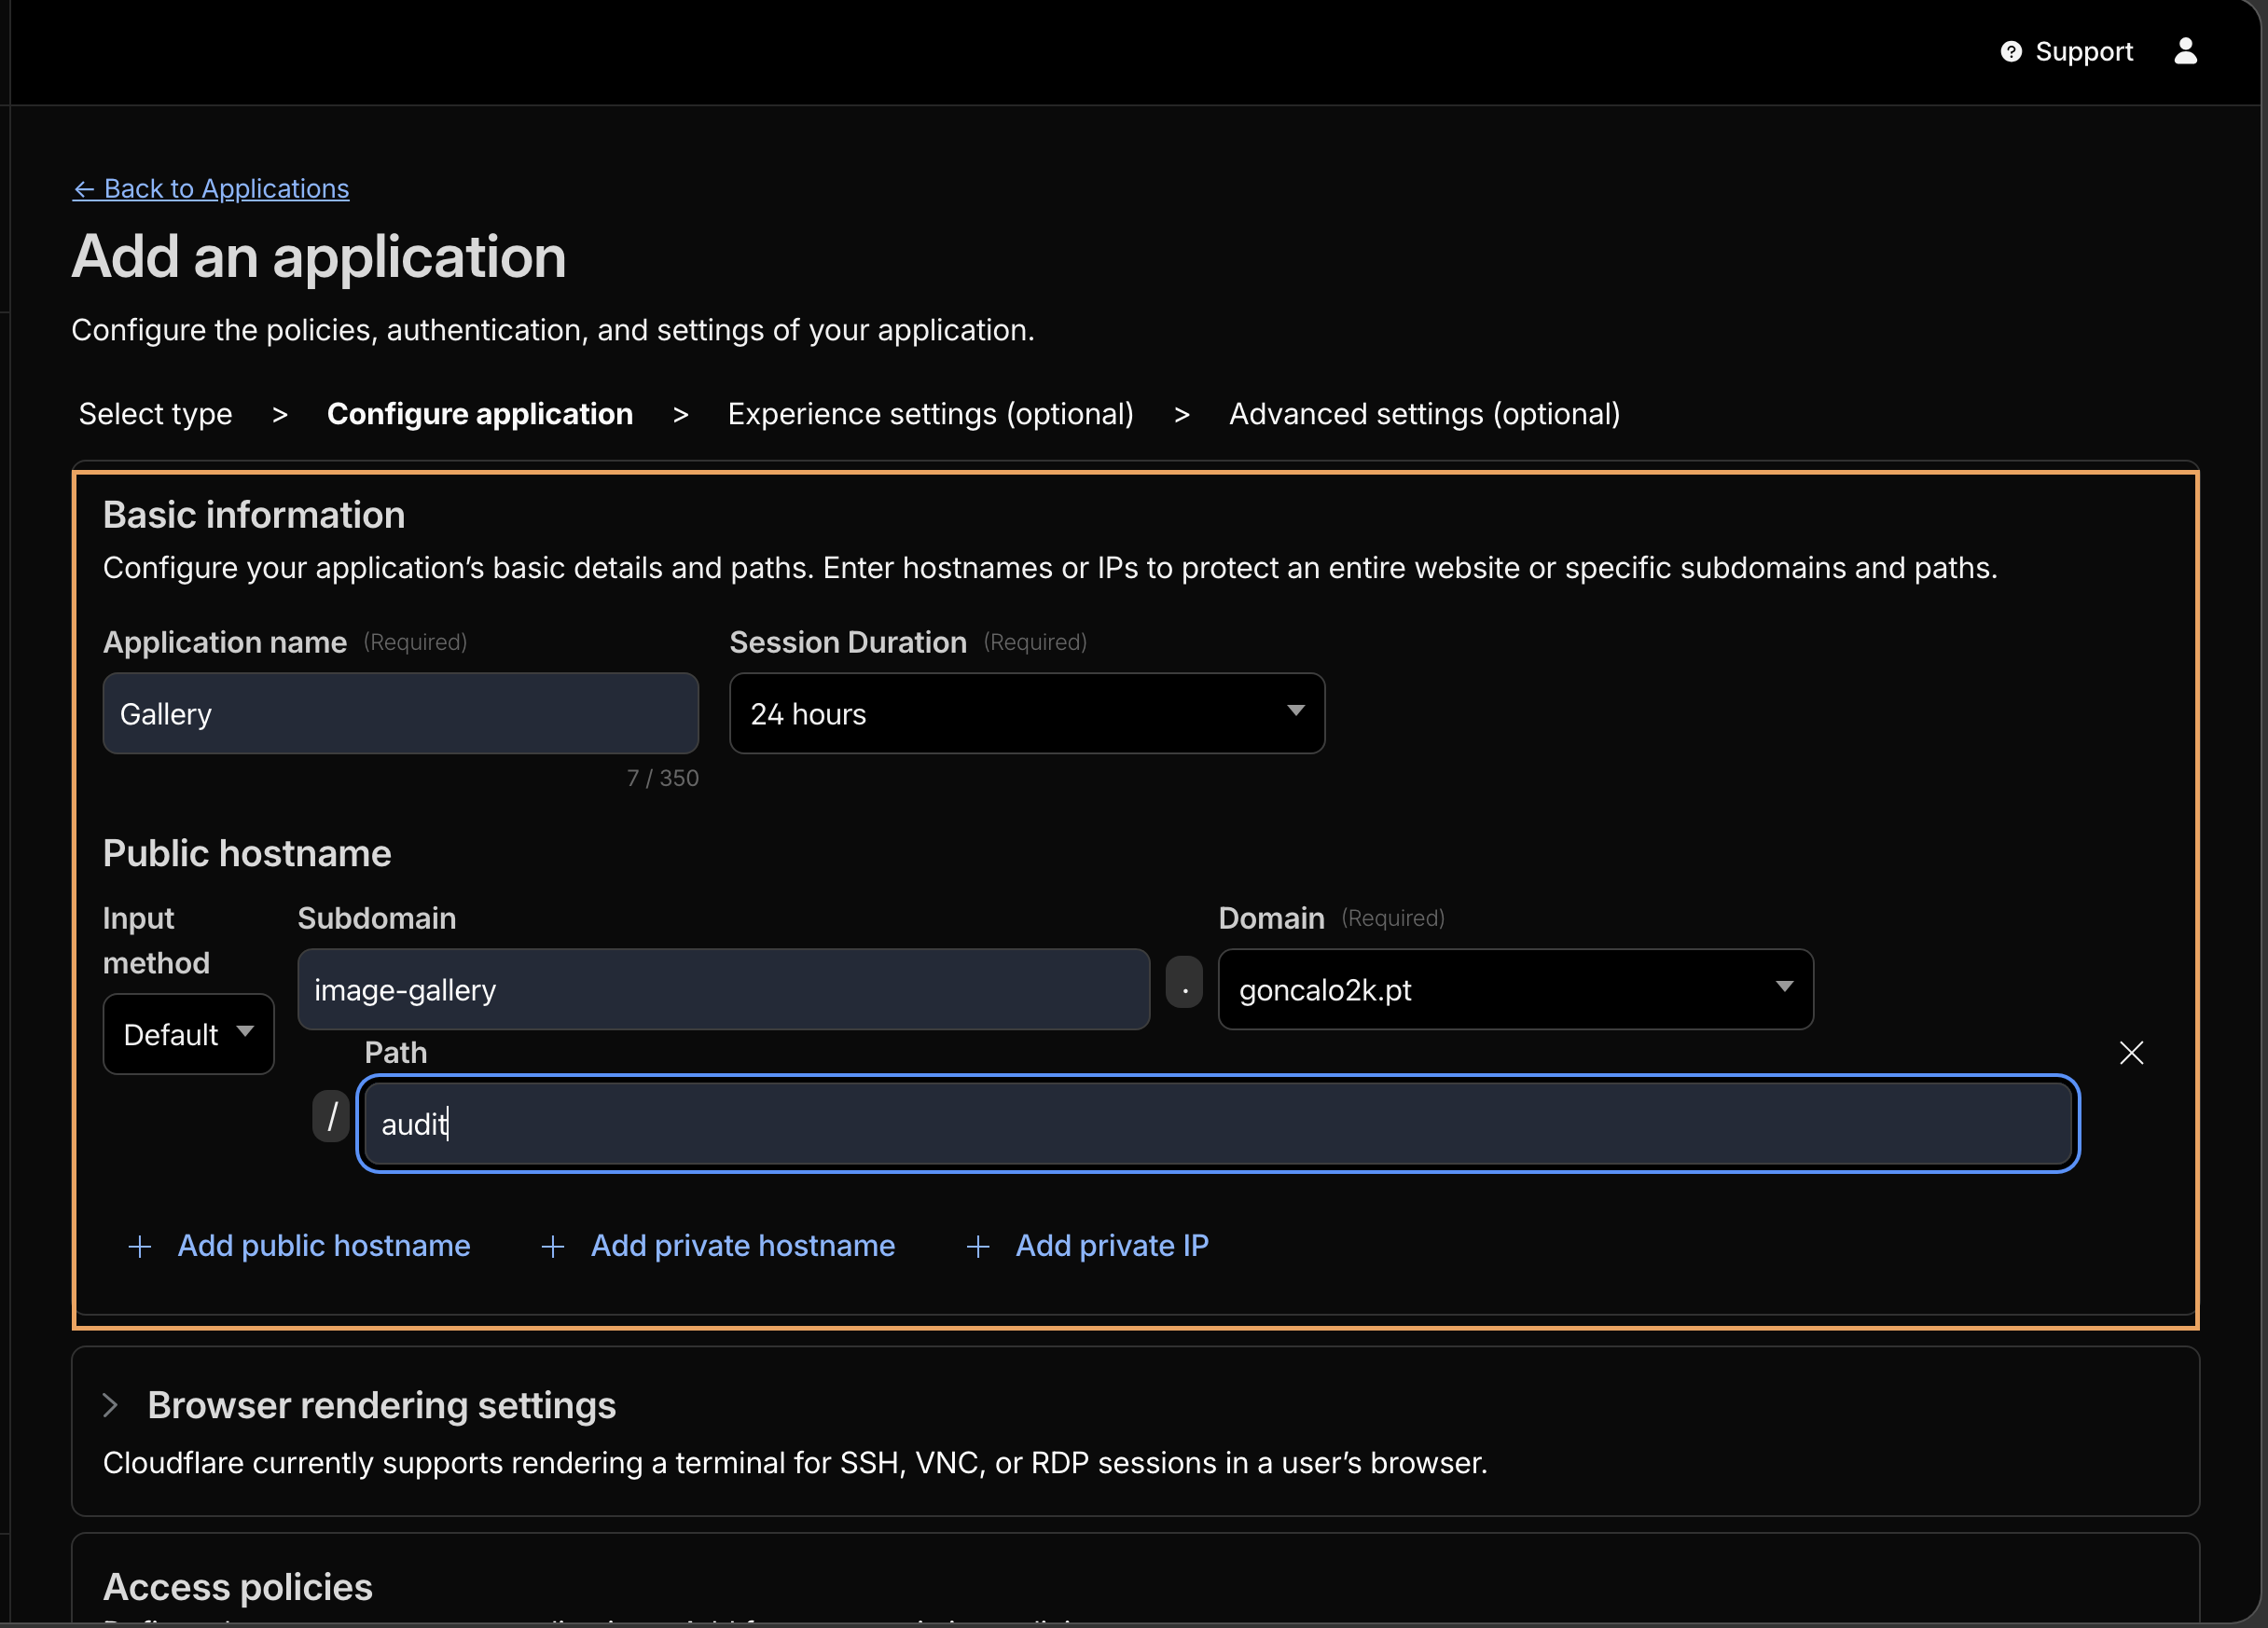
\includegraphics[width=0.5\textwidth]{media/zt/zt_4.png}
  \item Then, go on to \textbf{Access Policies} section and select an existing policy\\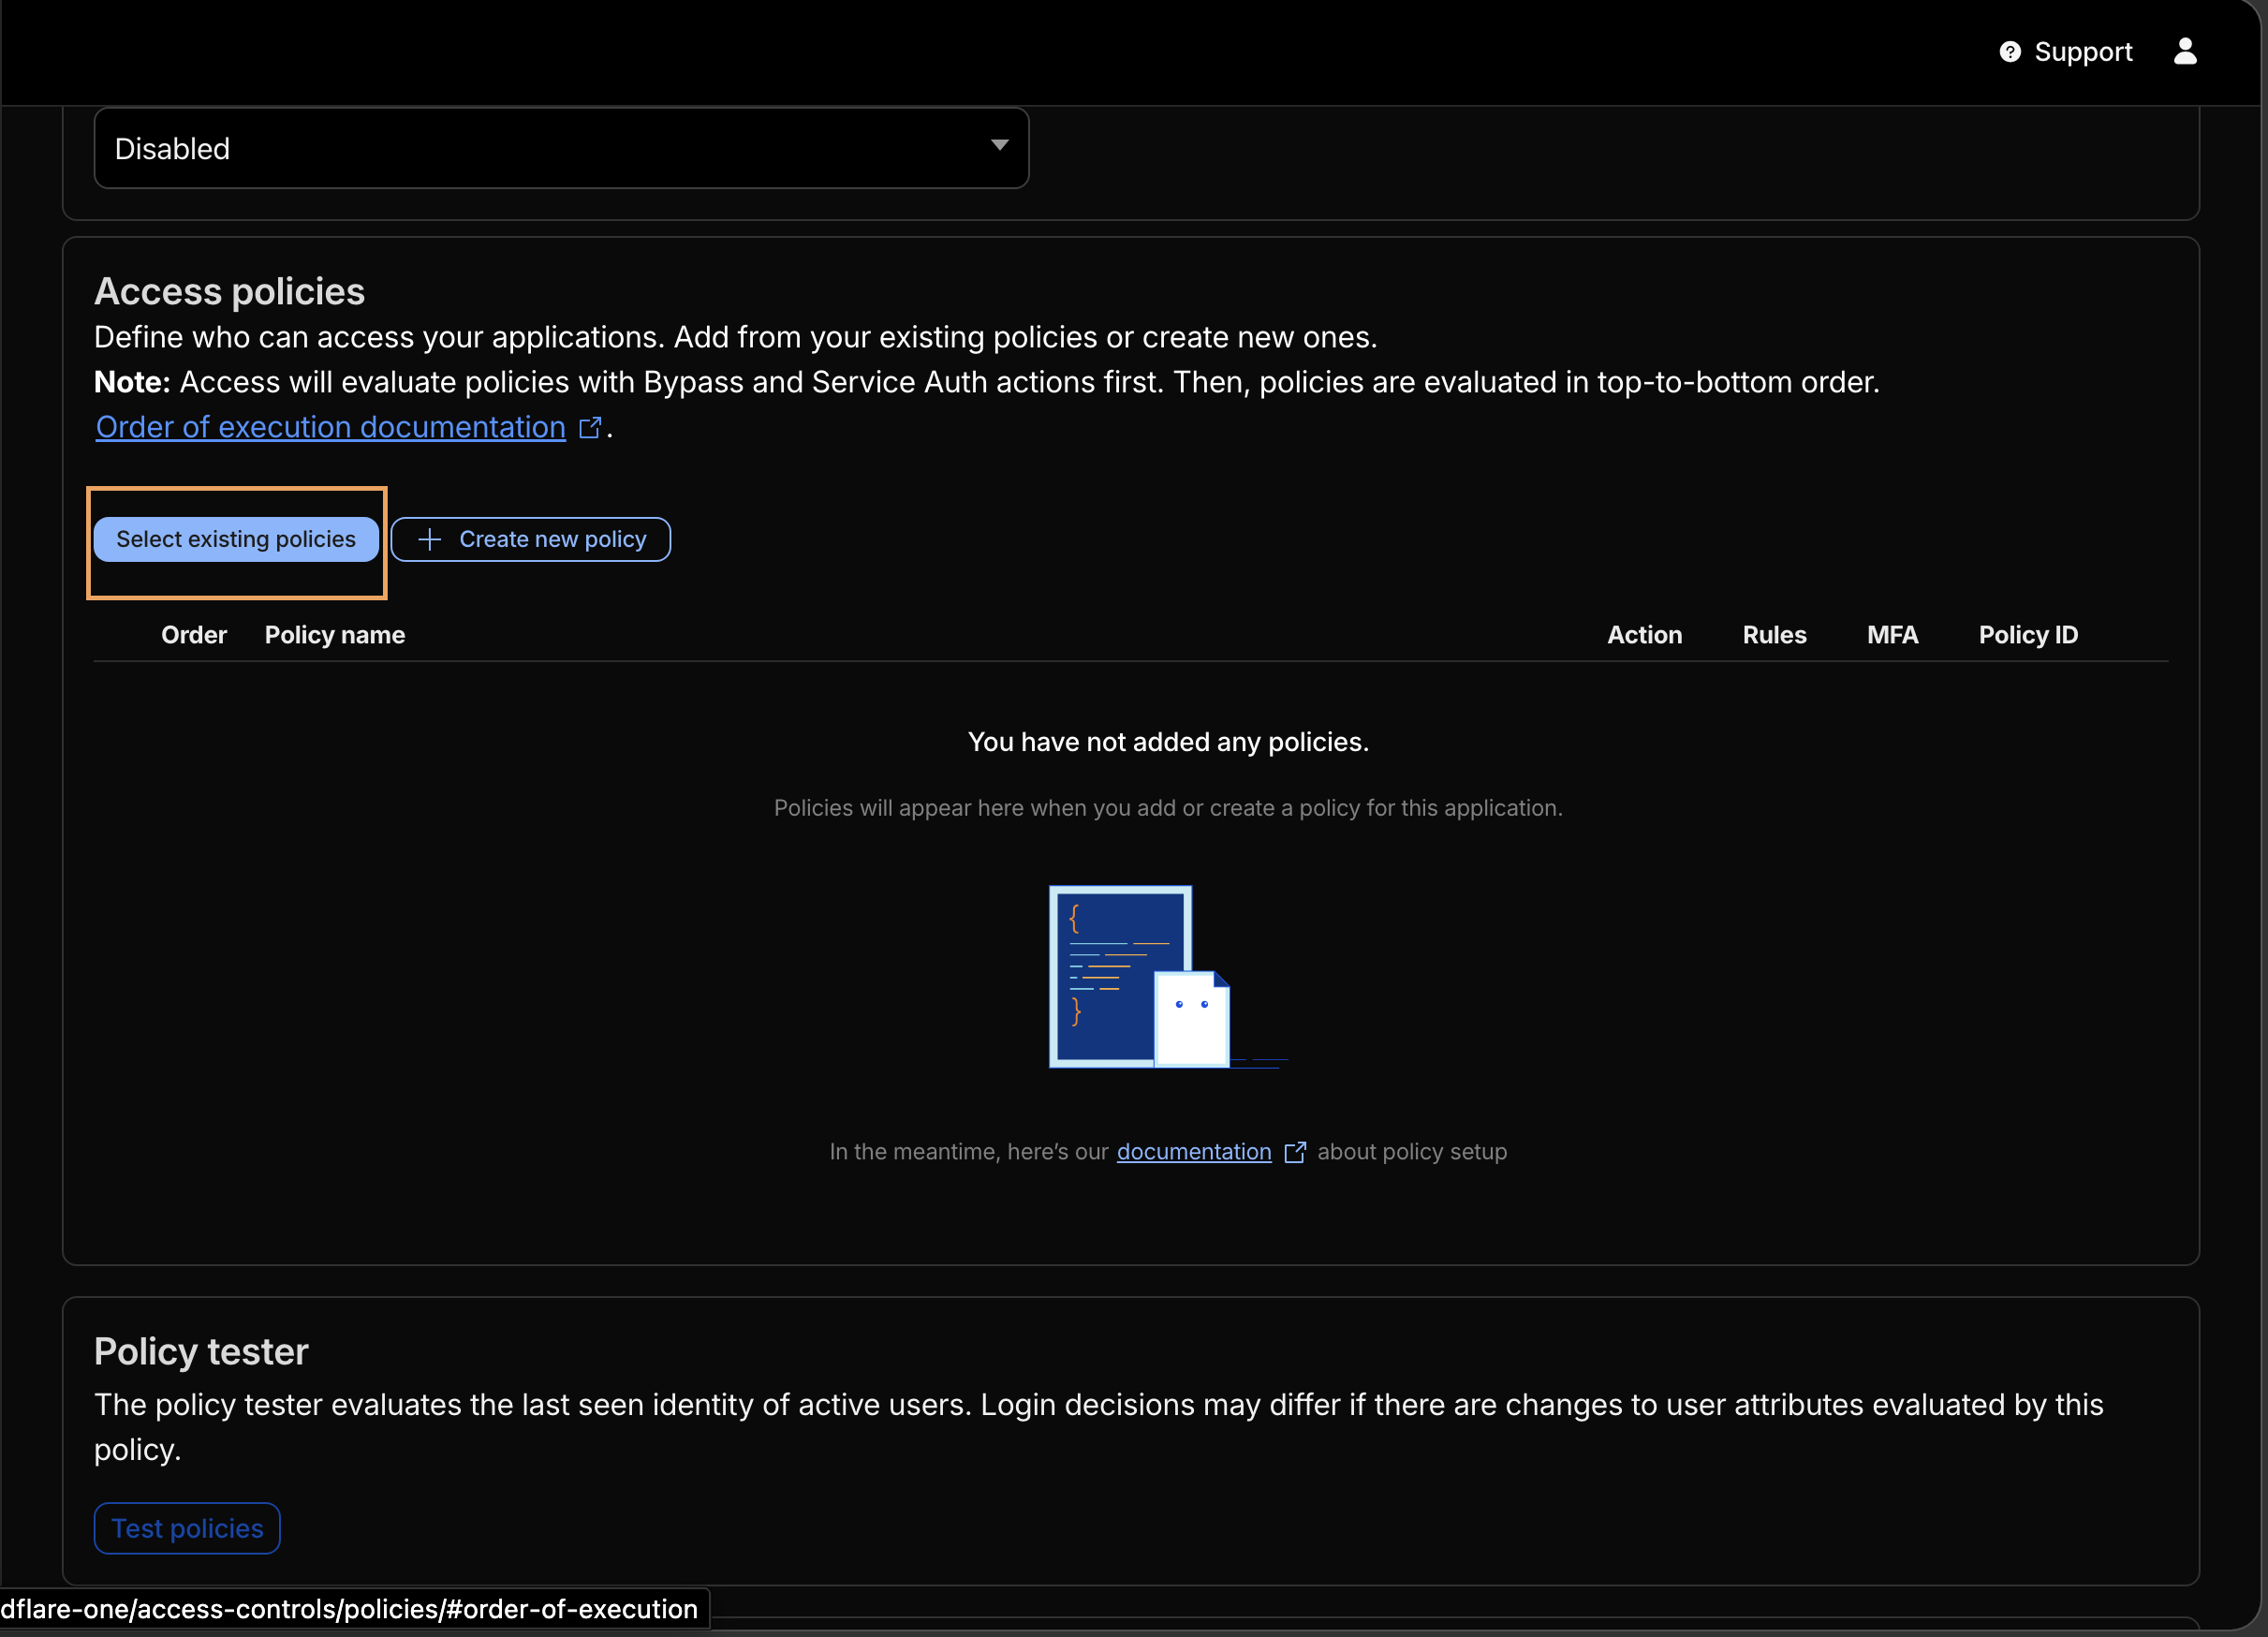
\includegraphics[width=0.5\textwidth]{media/zt/zt_5.png}
  \item Select the previously created policy\\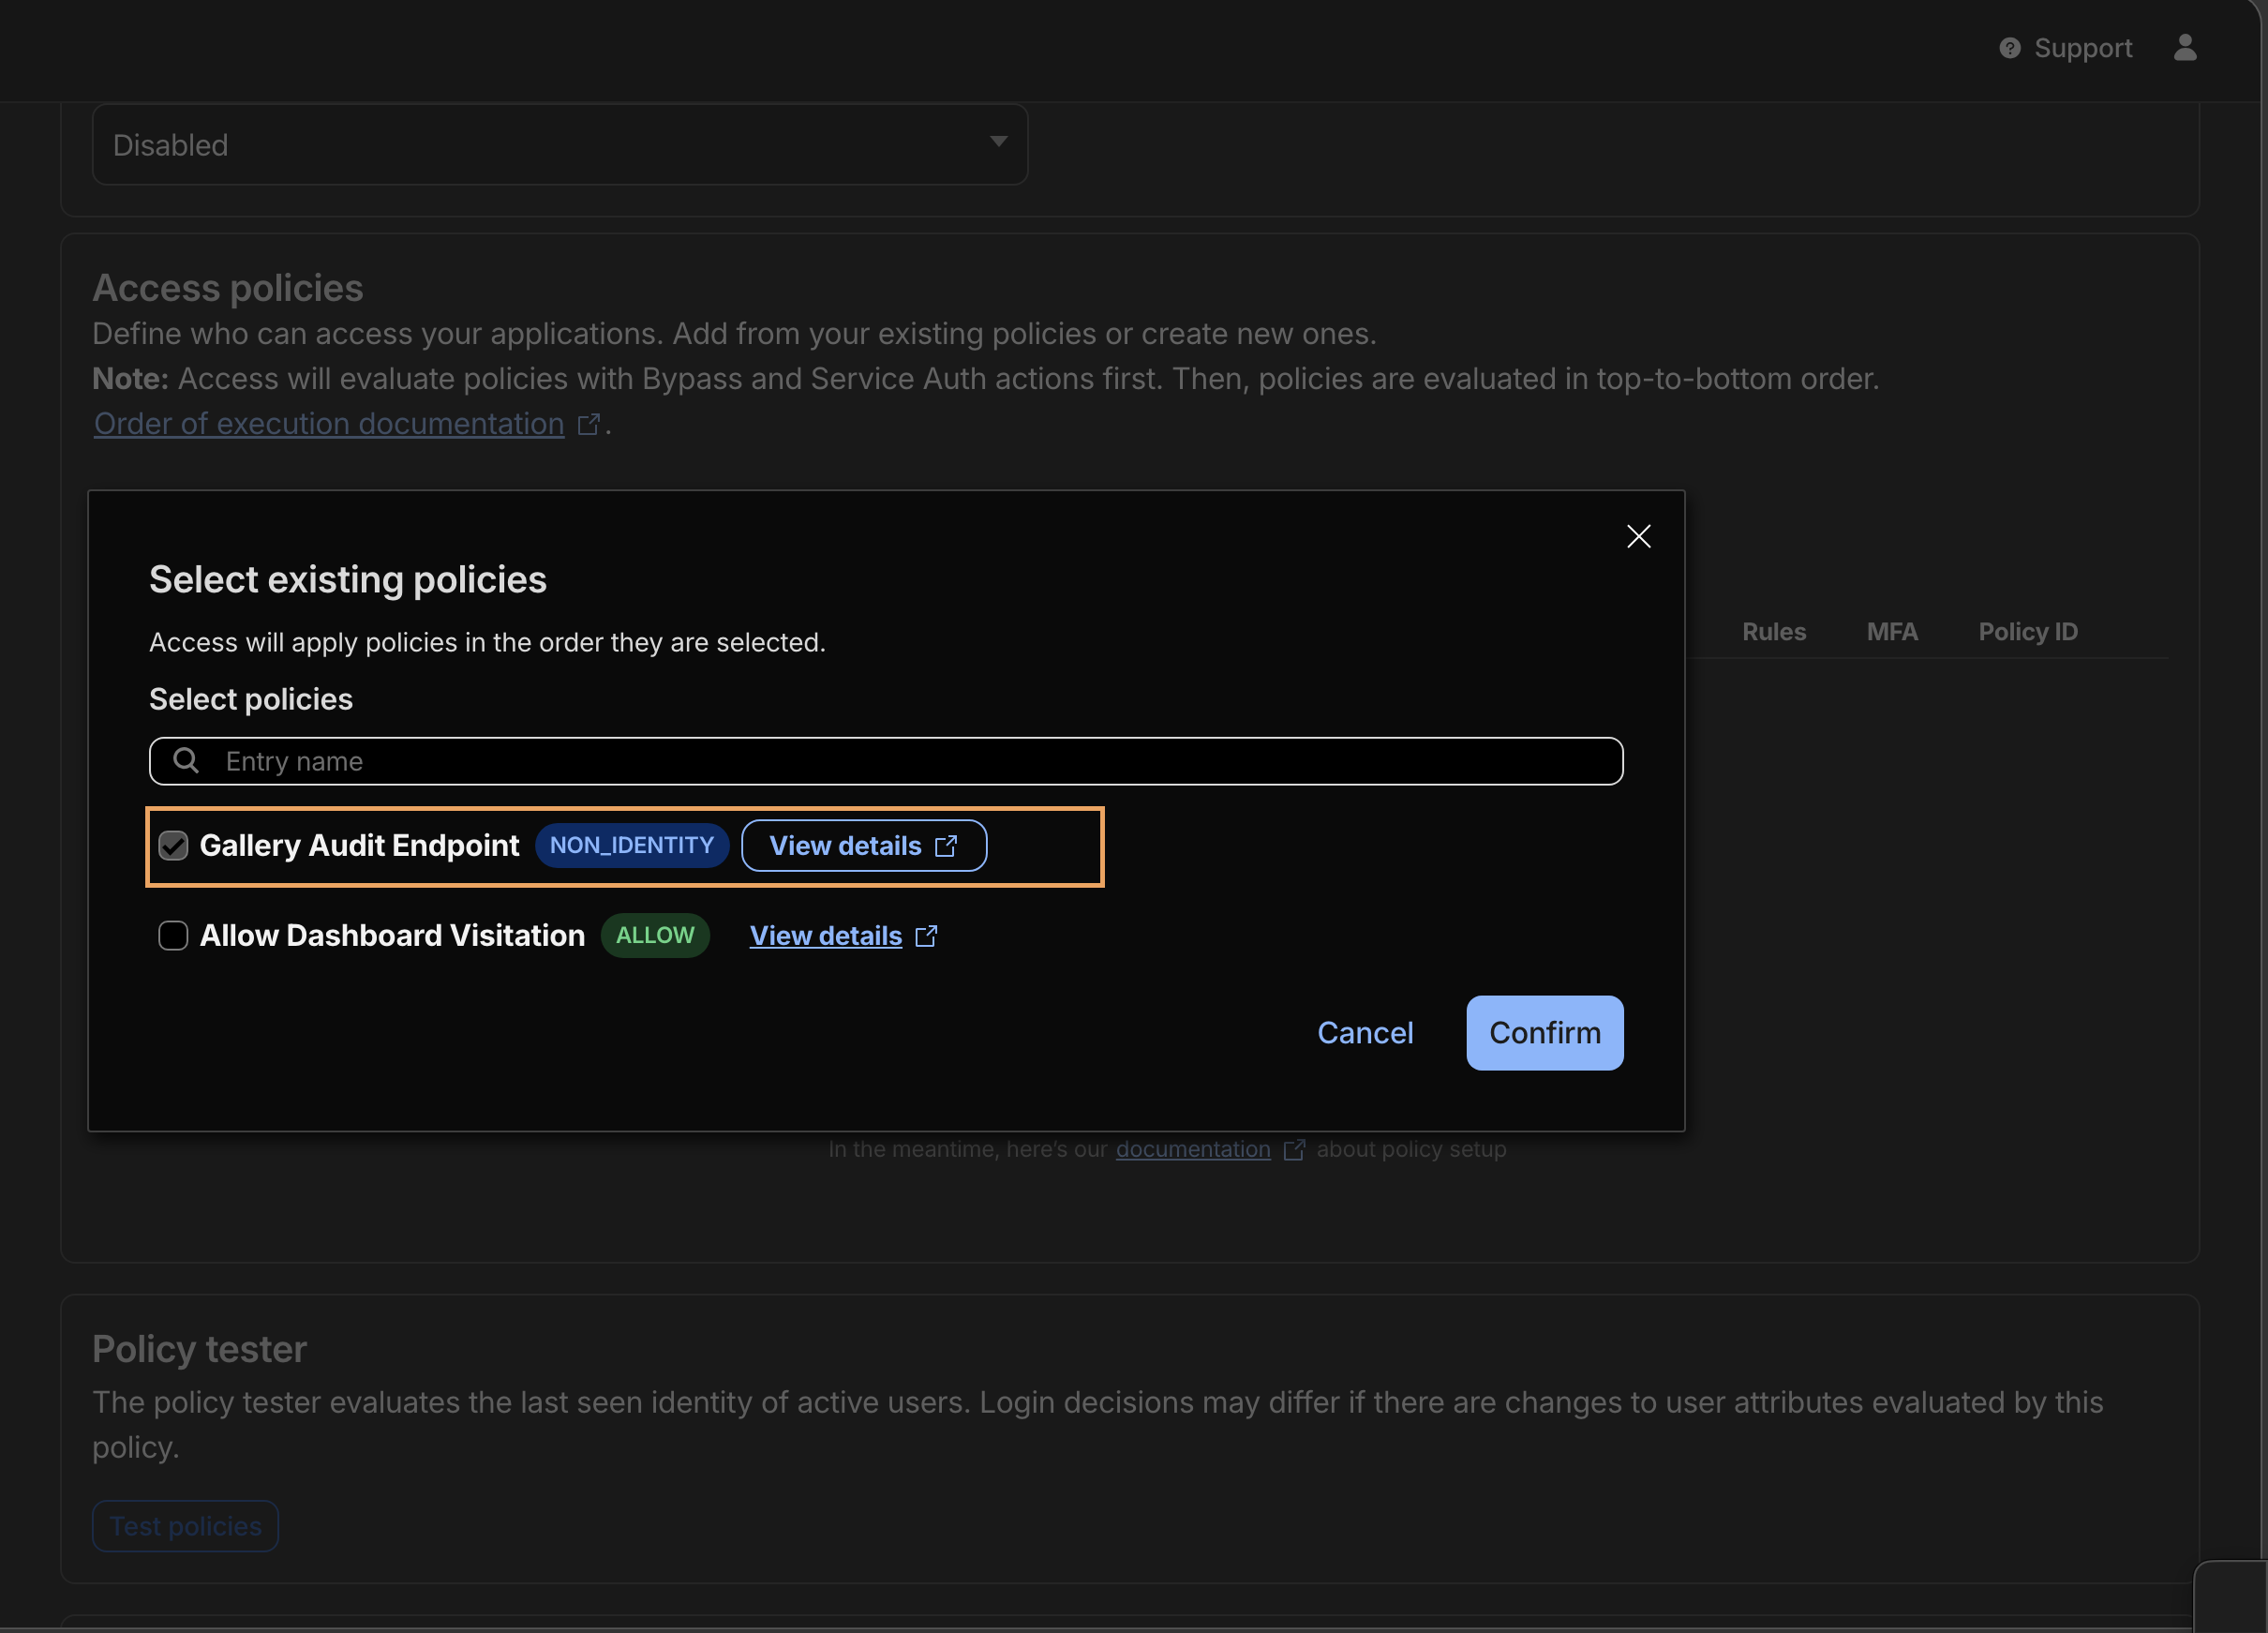
\includegraphics[width=0.5\textwidth]{media/zt/zt_6.png}
  \item Then hit \textbf{Next}\\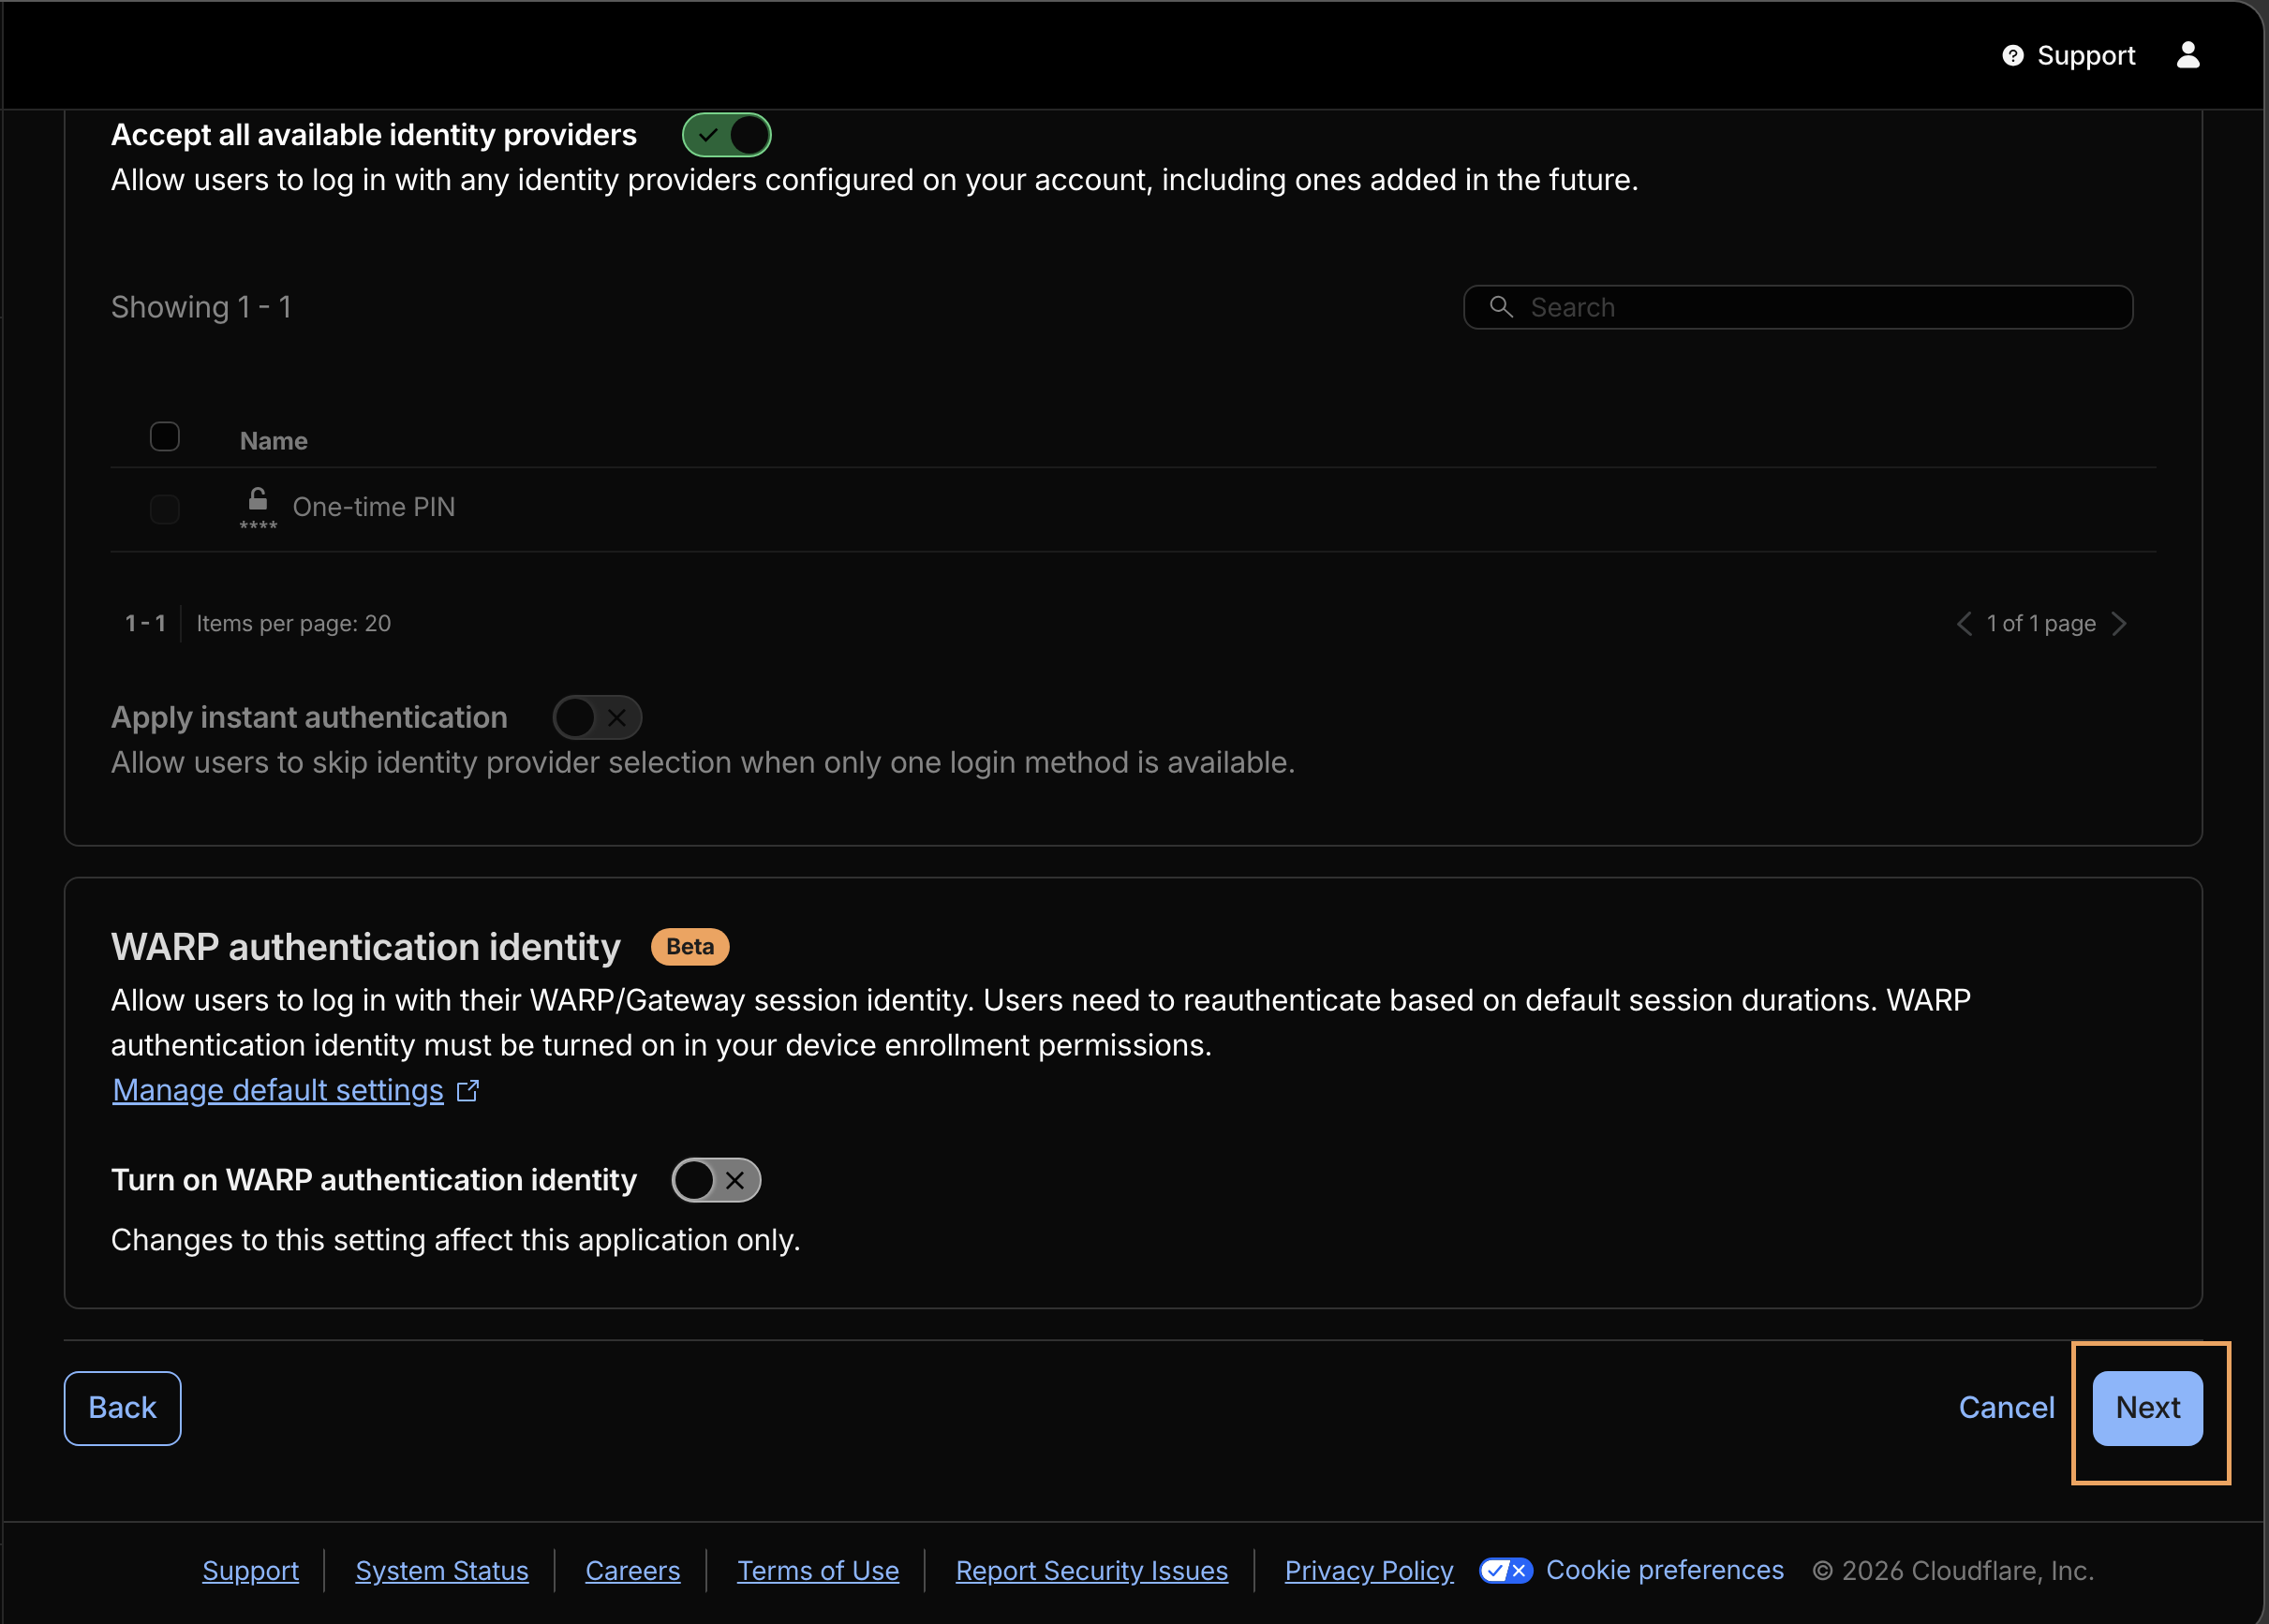
\includegraphics[width=0.5\textwidth]{media/zt/zt_7.png}
  \item In the \textbf{Advanced Settings}, turn on \textbf{401 Response for Service Auth policies}\\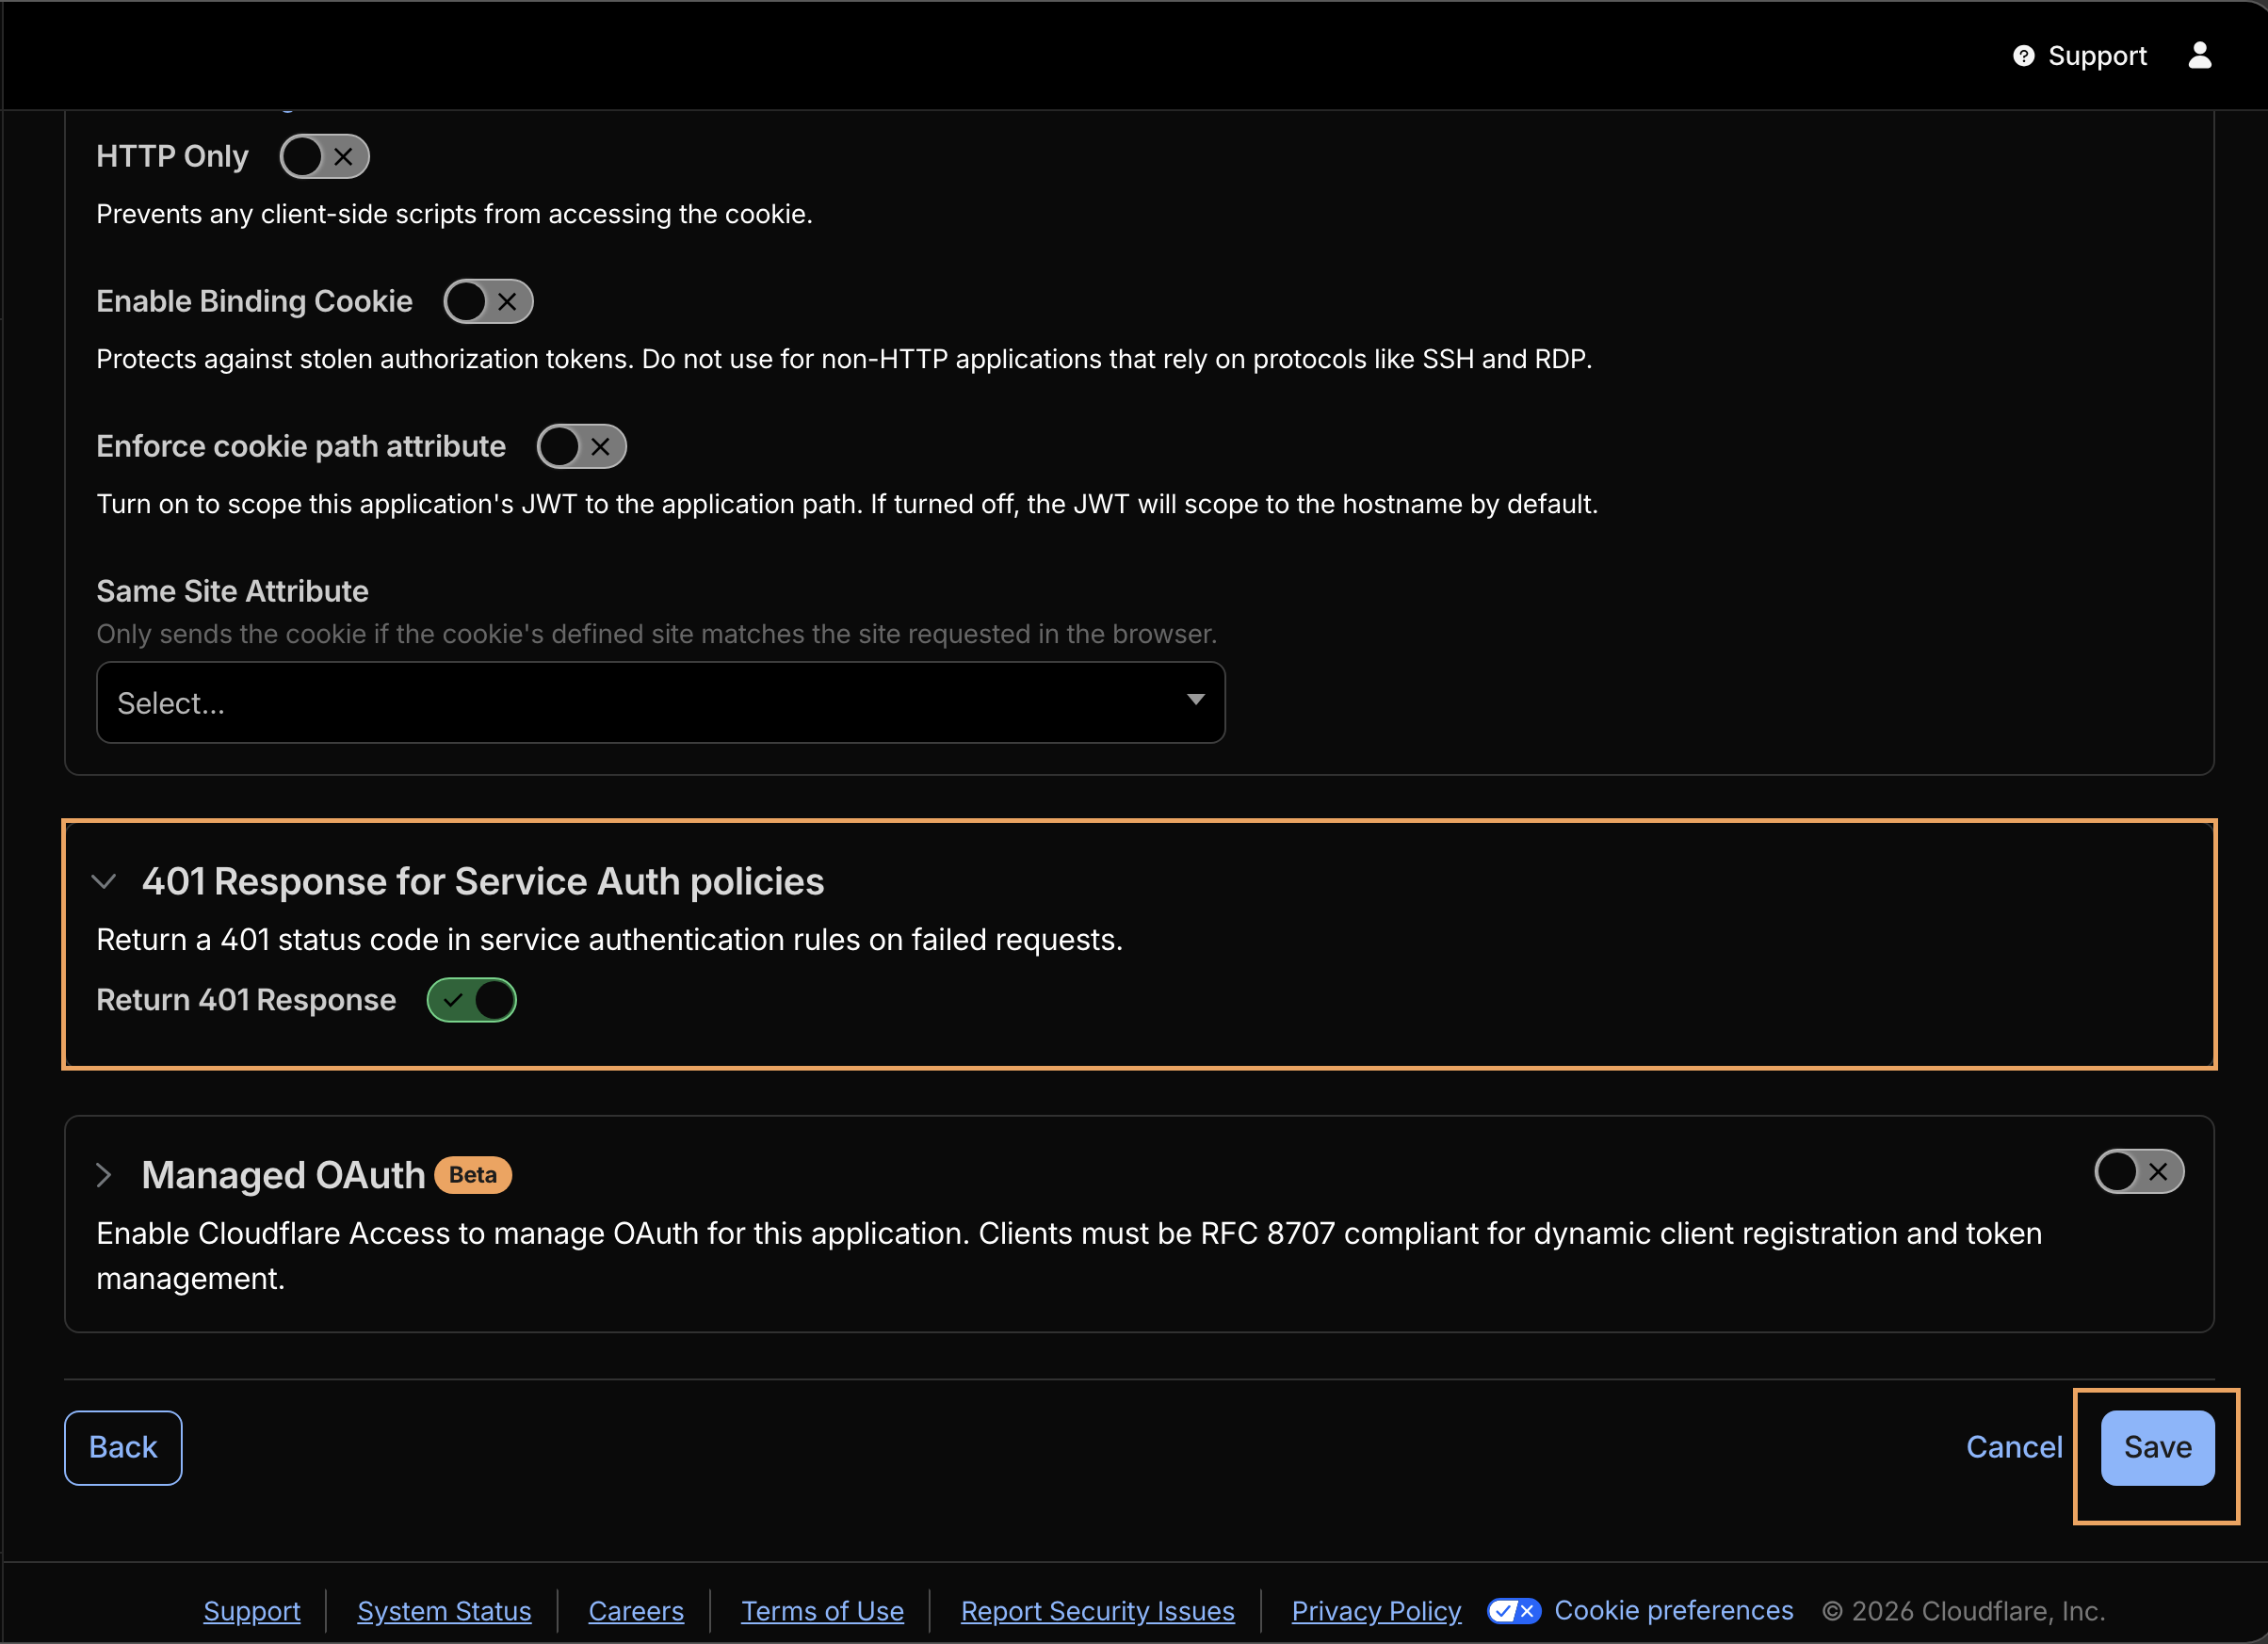
\includegraphics[width=0.5\textwidth]{media/zt/zt_8.png}
\end{enumerate}

\subsection{Worker Code Development}
Each handler exists for a specific operational need:
\begin{itemize}[leftmargin=*]
  \item \textbf{\texttt{GET /health} / \texttt{/docs} / \texttt{/openapi.json}} – Remain unauthenticated to support monitoring and human documentation access. Security middleware still applies headers, but \texttt{auth.middleware.ts} exits early for these paths so dashboards and Swagger UI render without tokens.
  \item \textbf{\texttt{GET /images}} – Lists metadata out of D1 using \texttt{offset}/\texttt{limit} sanitized by \texttt{getPaginationParams}. The rationale is to keep control planes lightweight: clients can paginate without worrying about \texttt{COUNT(*)} drift, and limit clamps ($\leq$100) prevent expensive scans.
  \item \textbf{\texttt{POST /images}} – Accepts uploads and enforces strict invariants before spending resources. Controllers verify only one \texttt{file} part exists, \texttt{ImageService} normalizes names to lowercase (deduping by logical name instead of random IDs), and MIME validation guarantees R2 never stores unsupported formats. Returning \textbf{200} when metadata already exists keeps uploads idempotent; returning \textbf{202} when a new asset enters the system acknowledges the blob write immediately while metadata inserts run via \texttt{executionCtx.waitUntil}, ensuring the client isn’t blocked by D1 latency. If that background write fails, the service deletes the blob to maintain consistency. To ensure the image was correctly uploaded, polling this endpoint can be an option - as soon as it responds with 200, the system is sure it was successfully uploaded both to R2 and to D1. This is a relatively common pattern, seen in \href{https://docs.github.com/en/rest/metrics/statistics?apiVersion=2026-03-10}{Github's REST API for statistics}, for example.
  \item \textbf{\texttt{POST /images/external}} – Mirrors the local file upload flow but first validates the URL with \texttt{parseHttpUrl} (http/https only, host required) and checks the upstream \texttt{content-type} header after fetching with redirects disabled. This endpoint exists in order to enable dynamic ingestion of assets without uploading files directly, while still benefiting from the same dedupe and MIME guardrails.
  \item \textbf{\texttt{GET /images/{id}}} – Streams binaries straight from the edge cache when possible; on cache miss it loads from R2, looks up metadata in D1, and sets \texttt{ALT\_HEADER\_NAME}, \texttt{Content-Type}, \texttt{Cache-Control}, and an immutable \texttt{ETag}. The cache entry key is the raw request URL, so variant paths don’t collide. This endpoint is the public face of the gallery, hence the extra emphasis on immutable headers and cache invalidation hooks.
  \item \textbf{\texttt{DELETE /images/{id}}} – Fan-outs to R2 and D1 with \texttt{Promise.allSettled}; if D1 reports \texttt{changes === 0}, the handler returns \textbf{404} and skips R2 cleanup (because nothing should exist). Successful deletions return \textbf{200} with no body, and a \texttt{waitUntil} call evicts the cached file to avoid stale responses. This keeps destructive operations fast while guaranteeing both data stores stay in sync.
  \item \textbf{\texttt{GET /images/audit}} – Protected by \texttt{auth.middleware.ts} because it exposes aggregate stats (\texttt{totalImages}, \texttt{lastUpdated}) and a paginated list of recent uploads. Same pagination helper enforces limits, and the response mirrors production monitoring needs (UI dashboards, CLI scripts). Keeping it read-only and authenticated balances observability with security.
  \item \textbf{Database Schema} – A single \texttt{images} table in D1 stores \{ \texttt{id TEXT PRIMARY KEY}, \texttt{name TEXT UNIQUE NOT NULL}, \texttt{description TEXT NOT NULL}, \texttt{content\_type TEXT}, \texttt{created\_at TEXT DEFAULT CURRENT\_TIMESTAMP} \} plus an index on \texttt{name}. That schema mirrors what the worker needs at runtime: the \texttt{name} uniqueness constraint implements deduplication for uploads, \texttt{created\_at} backs audit ordering and cache \texttt{ETag}s, and \texttt{content\_type} lets D1 remain the source of truth for MIME types. By keeping the table narrow this API can paginate and audit without scanning bloated rows. Besides this, the usage of an index on the \texttt{name} column enables faster queries when checking for already existing files by name (which is done on file upload).
\end{itemize}

Cross-cutting middleware reinforces these choices. \texttt{loggingMiddleware} injects/propagates \texttt{X-Correlation-Id} so every log line ties back to a single request (and downstream systems can pass their own IDs). \texttt{cors.middleware.ts} enforces allow-lists derived from \texttt{ALLOWED\_ORIGINS}, returning early when the \texttt{Origin} header is disallowed. \texttt{auth.middleware.ts} consults \texttt{AUTH\_ROUTES}: it skips open paths entirely, but when enabled it extracts user-provided headers (\texttt{CLIENT\_ID\_HEADER}, \texttt{CLIENT\_SECRET\_HEADER}), ensures both buffers are the same size, and then runs timing-safe equality checks so attackers can’t measure response time differences. \texttt{security-headers.middleware.ts} blankets every response with CSP, \texttt{X-Content-Type-Options}, and Referrer-Policy, etc., and only relaxes CSP for \texttt{/docs} so Swagger assets can load. And even outside middleware, \texttt{ImageService} includes safeguards such as rolling back R2 blobs if the metadata insert fails, which keeps storage in sync without manual cleanup. Together, these layers make the Worker predictable and safe: each endpoint is as open or locked down as intended, and any failure path still emits traceable logs.

\section{Performance Considerations}
The Worker architecture optimizes both latency and resource consumption:
\begin{enumerate}[leftmargin=*]
  \item \textbf{Edge caching as first hop} – \texttt{ImageController.getImage} hits \texttt{caches.default} before R2/D1 and caches successful responses with immutable TTLs and strong \texttt{ETag}s. Deletes schedule \texttt{caches.default.delete()} inside \texttt{executionCtx.waitUntil} to prevent stale assets lingering at the edge.
  \item \textbf{Parallel ingestion} – R2 uploads and Workers AI captioning run concurrently via \texttt{Promise.allSettled}. Deletions from R2 and D1 are also parallelized in the \texttt{/DELETE /images/:id}, speeding up deletions. Metadata writes upon file upload execute in \texttt{executionCtx.waitUntil}, so client requests only wait for blob persistence and caption generation, not D1 inserts. Finally, insertions and deletions from \texttt{Cloudlfare's CDN} are also done via non-blocking operations, enabling faster response times.
  \item \textbf{Smart payload bounds} – \texttt{MAX\_UPLOAD\_SIZE\_MB} guards uploads, while \texttt{resizeImageForAI} uses the Images binding to downscale >1 MB buffers to 1024×1024 JPEGs, reducing inference cost and allowing the AI models to process all images sent within the 20MB range.
  \item \textbf{Efficient pagination} – \texttt{getPaginationParams} sanitizes \texttt{offset}/\texttt{limit} (max 100) for \texttt{/images} and \texttt{/images/audit}, avoiding large scans. Prepared statements reuse query plans, keeping D1 latency steady.
  \item \textbf{Streamed delivery} – Downloaded R2 objects are wrapped in \texttt{File} instances and streamed to the client, so Workers can start sending bytes immediately instead of buffering entire images.
  \item \textbf{Operational throttling} – Automation scripts (\texttt{scripts/batch-upload.mjs}, \texttt{scripts/clear-all-images.mjs}) expose concurrency/delay knobs, ensuring bulk jobs do not overwhelm the Worker or exceed API quotas.
\end{enumerate}

\section{Knowledge Gaps and Learning Process}
Despite previous experience with Cloudflare Workers, several capabilities required deeper research before implementing the final solution. Each gap below lists the referenced material and the concrete takeaway that shaped the codebase.
\begin{enumerate}[leftmargin=*]
  \item \textbf{Workers AI pipeline design} – The \href{https://developers.cloudflare.com/use-cases/ai/}{Workers AI use-case catalog} clarified how to use Workers AI and all the necessary models from Workers, what payload shapes they expect, and how to stay within neuron budgets (capping token counts was the chosen approach). This guided the \texttt{ImageService.generateImageAltText} implementation. However, it soon became obvious that images over a few bytes would be problematic, as the AI model in use (\href{https://developers.cloudflare.com/workers-ai/models/llava-1.5-7b-hf/}{llava-1.5-7b-hf}) didn't accept such files. For this, Transform Image's worker binding was used to resize images and the smaller, resized buffers were utilized for the inference.
  \item \textbf{D1 query ergonomics} – The \href{https://developers.cloudflare.com/d1/}{D1 documentation} explained prepared statements, result helpers (\texttt{.first()}, \texttt{.run()}), and schema deployment flows. Those patterns are used in every metadata access path. In addition, the \texttt{pnpm run setup-local-db} / \texttt{deploy-db} scripts are also based in D1 functions, by using the API's endpoints.
  \item \textbf{R2 usage from Workers} – The \href{https://developers.cloudflare.com/r2/api/workers/workers-api-usage/}{R2 Workers API reference} was key to understand how the \texttt{R2Bucket}binding works and how uploads, fetches and deletions work within a Worker's context.
  \item \textbf{Typed bindings} – The Worker best-practices note on \href{https://developers.cloudflare.com/workers/best-practices/workers-best-practices/#generate-binding-types-with-wrangler-types}{wrangler types} showed how to auto-generate \texttt{worker-configuration.d.ts}, which led to the \texttt{pnpm run cf-typegen} script and the strongly typed \texttt{AppEnv} interface.
  \item \textbf{Edge caching semantics} – Building \texttt{ImageController.getImage} required revisiting the \href{https://developers.cloudflare.com/workers/runtime-apis/cache/}{Cache API docs} to confirm how \texttt{caches.default.put()} behaves within \texttt{waitUntil}, what are good practices in key-creation, what cache strategies can be implemented and how cache invalidation can be done (in this case, after deletions).
  \item \textbf{Execution context guarantees} – The \href{https://developers.cloudflare.com/workers/runtime-apis/context/}{Context API reference} clarified how non-blocking operations can be leverage in Workers, via \texttt{executionCtx.waitUntil}, as this may extend a worker's lifetime for another extra 30 seconds, reinforcing the decision to offload D1 writes and cache invalidations into that lifecycle hook, enabling the API to have faster response times.
  \item \textbf{Timing-safe auth} – To harden \texttt{/images/audit} and any protected routes, the Worker follows the \href{https://developers.cloudflare.com/workers/examples/protect-against-timing-attacks/}{timing-attack protection example} by comparing credentials with \texttt{crypto.subtle.timingSafeEqual}, preventing side-channel leaks even when headers are incorrect.
\end{enumerate}

Documenting these learnings ensures future contributors know which Cloudflare primitives influenced each architectural decision and where to dig deeper when requirements evolve.

\section{Security Considerations}
Security spans middleware, bindings, and operational guardrails:
\begin{enumerate}[leftmargin=*]
  \item \textbf{Authenticated admin routes} – \texttt{auth.middleware.ts} inspects \texttt{CF-Access-Client-Id} / \texttt{CF-Access-Client-Secret}, enforces timing-safe comparisons with \texttt{crypto.subtle.timingSafeEqual}, and scopes protection via \texttt{AUTH\_ROUTES} so sensitive endpoints (e.g., \texttt{/images/audit}) require valid service tokens.
  \item \textbf{Least-privilege bindings} – \texttt{wrangler.jsonc} binds only the required resources (R2, D1, Images, AI) plus explicit env vars. Secrets never live in code, and \texttt{.dev.vars.example} documents placeholders so local dev mirrors production without credential reuse.
  \item \textbf{Request hygiene} – \texttt{cors.middleware.ts} parses \texttt{ALLOWED\_ORIGINS} CSV allow-lists, rejecting disallowed origins. \texttt{security-headers.middleware.ts} adds CSP, \texttt{X-Content-Type-Options}, and \texttt{Referrer-Policy}, relaxing CSP solely for \texttt{/docs} so Swagger assets can load safely.
  \item \textbf{Data consistency \& cache cleanup} – Delete operations fan out to R2 + D1 via \texttt{Promise.allSettled}, and cache entries are purged asynchronously with \texttt{executionCtx.waitUntil(caches.default.delete(...))}, preventing orphaned binaries or stale public responses.
  \item \textbf{Input validation} – \texttt{isValidImageName}, \texttt{MAX\_UPLOAD\_SIZE\_MB}, and strict MIME checks on external ingestion prevent malformed uploads. FormData mappers normalize names to lowercase to avoid duplicates with different casing.
  \item \textbf{Structured logging} – \texttt{loggingMiddleware} issues correlation IDs per request, and the Pino logger redacts sensitive headers, enabling auditing without exposing secrets.
\end{enumerate}

\end{document}
